\documentclass[12pt]{report}\usepackage[]{graphicx}\usepackage[dvipsnames]{xcolor}
% maxwidth is the original width if it is less than linewidth
% otherwise use linewidth (to make sure the graphics do not exceed the margin)
\makeatletter
\def\maxwidth{ %
  \ifdim\Gin@nat@width>\linewidth
    \linewidth
  \else
    \Gin@nat@width
  \fi
}
\makeatother

\definecolor{fgcolor}{rgb}{0.345, 0.345, 0.345}
\newcommand{\hlnum}[1]{\textcolor[rgb]{0.686,0.059,0.569}{#1}}%
\newcommand{\hlstr}[1]{\textcolor[rgb]{0.192,0.494,0.8}{#1}}%
\newcommand{\hlcom}[1]{\textcolor[rgb]{0.678,0.584,0.686}{\textit{#1}}}%
\newcommand{\hlopt}[1]{\textcolor[rgb]{0,0,0}{#1}}%
\newcommand{\hlstd}[1]{\textcolor[rgb]{0.345,0.345,0.345}{#1}}%
\newcommand{\hlkwa}[1]{\textcolor[rgb]{0.161,0.373,0.58}{\textbf{#1}}}%
\newcommand{\hlkwb}[1]{\textcolor[rgb]{0.69,0.353,0.396}{#1}}%
\newcommand{\hlkwc}[1]{\textcolor[rgb]{0.333,0.667,0.333}{#1}}%
\newcommand{\hlkwd}[1]{\textcolor[rgb]{0.737,0.353,0.396}{\textbf{#1}}}%
\let\hlipl\hlkwb

\usepackage{framed}
\makeatletter
\newenvironment{kframe}{%
 \def\at@end@of@kframe{}%
 \ifinner\ifhmode%
  \def\at@end@of@kframe{\end{minipage}}%
  \begin{minipage}{\columnwidth}%
 \fi\fi%
 \def\FrameCommand##1{\hskip\@totalleftmargin \hskip-\fboxsep
 \colorbox{shadecolor}{##1}\hskip-\fboxsep
     % There is no \\@totalrightmargin, so:
     \hskip-\linewidth \hskip-\@totalleftmargin \hskip\columnwidth}%
 \MakeFramed {\advance\hsize-\width
   \@totalleftmargin\z@ \linewidth\hsize
   \@setminipage}}%
 {\par\unskip\endMakeFramed%
 \at@end@of@kframe}
\makeatother

\definecolor{shadecolor}{rgb}{.97, .97, .97}
\definecolor{messagecolor}{rgb}{0, 0, 0}
\definecolor{warningcolor}{rgb}{1, 0, 1}
\definecolor{errorcolor}{rgb}{1, 0, 0}
\newenvironment{knitrout}{}{} % an empty environment to be redefined in TeX

\usepackage{alltt}

\usepackage[spanish]{babel}
\usepackage[margin = 2.54cm]{geometry}
\usepackage[dvipsnames]{xcolor}
\usepackage{amssymb, amsthm, enumitem, fancyhdr, float, graphicx, hyperref, hologo, listings, mathtools, tikz, tikz-cd}
\usepackage[spanish, noabbrev]{cleveref}

\pagestyle{fancy}
\lhead{\footnotesize \leftmark}
\rhead{\footnotesize \rightmark}

\lstdefinestyle{estilo_pablo}{
	basicstyle = \ttfamily\footnotesize, 
	tabsize = 2, 
	commentstyle = \color{gray}, 
	keywordstyle = \color{cyan}, 
	stringstyle = \color{purple}, 
	tabsize = 1, 
	frame = tb, 
	breaklines = true, 
	showstringspaces = false, 
	numbers = left, 
	numberstyle = \footnotesize\color{gray}, 
	stepnumber = 1, 
	captionpos = b
}

\crefname{listing}{Código}{Códigos}
\crefname{section}{Sección}{Secciones}

\title{
	\huge
	\noindent\textbf{Fundamentos de la Ciencia de Datos}\\
	
	{\Large \textit{Práctica 1}}
	\vspace{1cm}
	
	\huge
	Grado en Ingeniería Informática\\
	Universidad de Alcalá\\
	
	\vspace{1cm}
	
	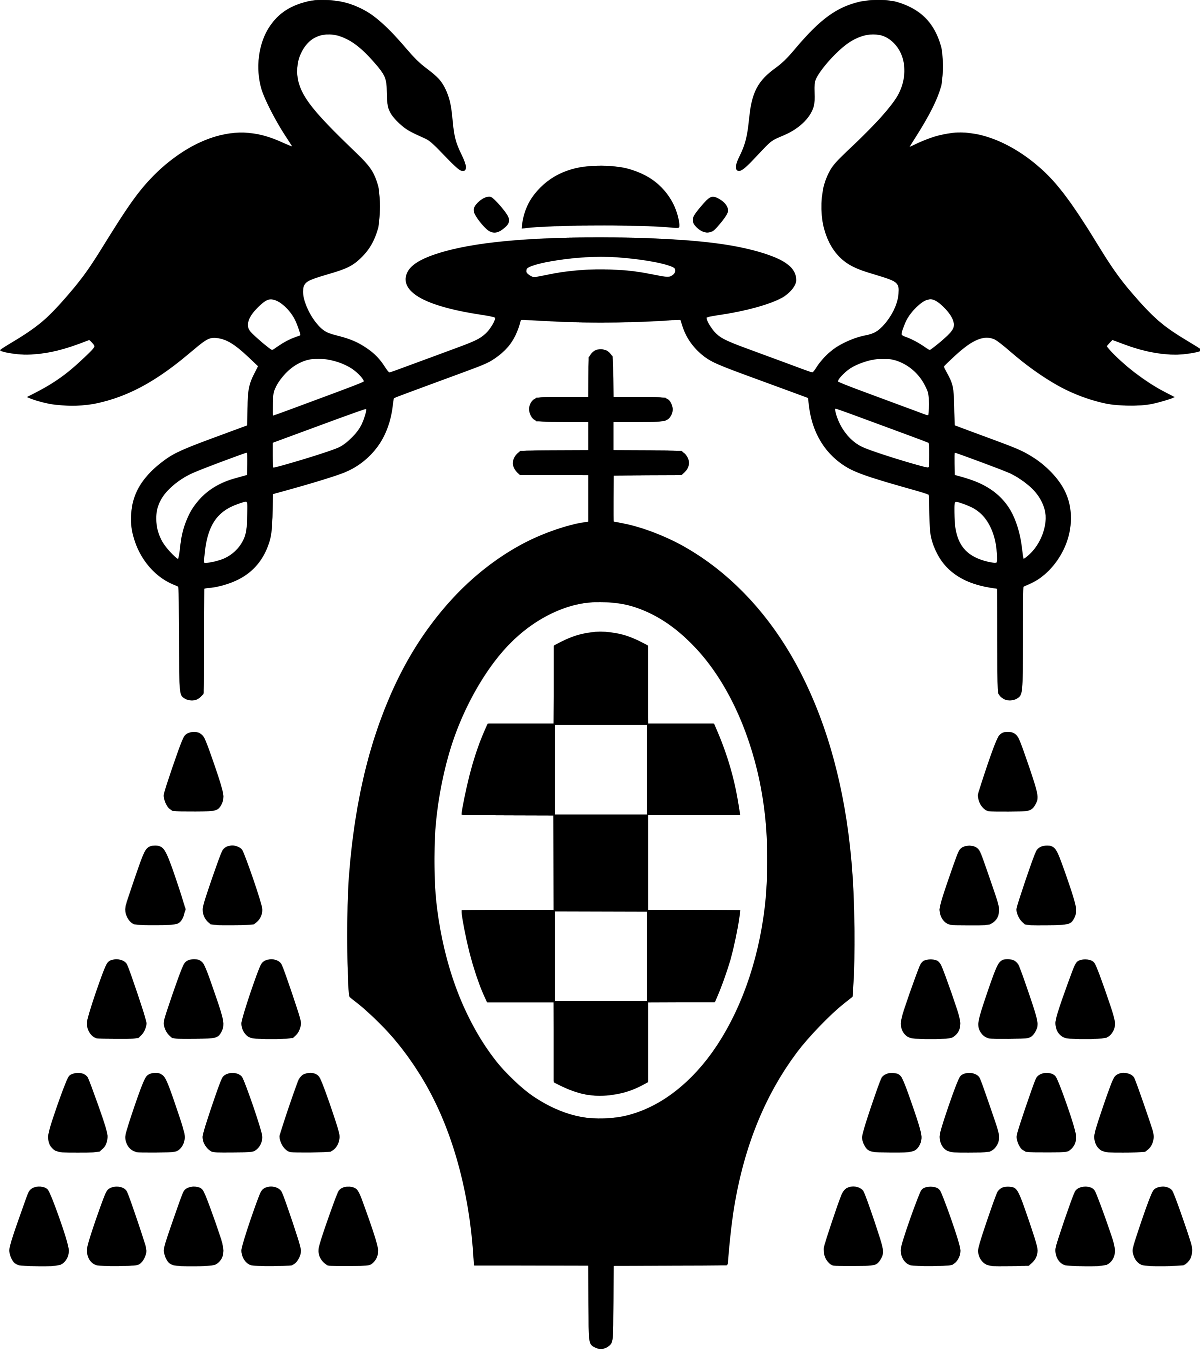
\includegraphics[scale = 0.075]{img/logo}
}

\author{
	Pablo García García\\
	Abel López Martínez\\
	Álvaro Jesús Martínez Parra\\
	Raúl Moratilla Núñez
}

\date{
	\large{14 de noviembre de 2023}
}

\hypersetup{
	pdftitle = {Práctica 1}, 
	pdfauthor = {Pablo García García, Abel López Martínez, Álvaro Jesús Martínez Parra, Raúl Moratilla Núñez}, 
	pdfsubject = {Fundamentos de la Ciencia de Datos}, 
	pdfcenterwindow, 
	pdfnewwindow = true, 
	pdfkeywords = {Entrega de la PL1 de laboratorio correspondiente al Curso 2023-2024}, 
	bookmarksopen = true 
}

\newtheorem{exercise}{Ejercicio}[section]

\newcommand{\dt}{\text{dist}}
\newcommand{\ds}{\text{dens}}
\newcommand{\drm}{\text{drm}}
\IfFileExists{upquote.sty}{\usepackage{upquote}}{}
\begin{document}
	
	\renewcommand{\chaptername}{Parte}
	\renewcommand{\lstlistingname}{Código}
	\maketitle \thispagestyle{empty}
	
	\newpage
	
	\setcounter{tocdepth}{3}
	\tableofcontents
	\listoffigures
	
	\chapter*{Introducción}\addcontentsline{toc}{chapter}{Introducción}\pagestyle{plain}
	
		\section*{El lenguaje R}\addcontentsline{toc}{section}{El lenguaje R}
		
			El lenguaje R, es un software de uso gratuito comúnmente usado en tareas relacionadas con la estadística, como el análisis o visualización de datos; o en general la propia Ciencia de Datos. Para ello cuenta con una gran cantidad de paquetes y herramientas que facilitan el trabajo.  
			
			\begin{figure}[H]
				\centering
				
\includegraphics[scale = 0.15]{img/Rlogo}
				\caption{Logo del lenguaje R}
				\label{fig:logo_R}
			\end{figure}
		
			El CRAN (Comprehensive R Archive Network, \url{https://cran.r-project.org/}) es un repositorio de recursos en línea que se utiliza para facilitar la distribución, el intercambio y el acceso a una amplia gama de software y paquetes relacionados con el lenguaje de programación R. La página web de CRAN sirve como el portal central para acceder a estos recursos y ofrece una variedad de apartados y enlaces útiles para los usuarios de R. A continuación, proporcionamos una descripción de los distintos enlaces a los que se puede acceder desde la página principal del CRAN: 
			
			\begin{itemize}
				\item Mirrors: Esta sección permite a los usuarios seleccionar un espejo (mirror) cercano para descargar paquetes y recursos. Los espejos son servidores que almacenan copias de los paquetes y datos de CRAN, lo que ayuda a mejorar la velocidad de descarga y la disponibilidad de los recursos.
				
				\item What's new?: En esta sección, los usuarios pueden encontrar información sobre las últimas actualizaciones y novedades en el mundo de R y los paquetes disponibles en CRAN. Esto es útil para estar al tanto de las últimas características y mejoras.
				
				\item Search: El enlace ``Search'' permite a los usuarios buscar paquetes y recursos específicos en el repositorio de CRAN. Además, se puede utilizar la función de búsqueda avanzada del motor de búsqueda de Google.
				
				\item CRAN Team: Aquí se puede encontrar información sobre las personas y equipos que trabajan en el mantenimiento y desarrollo de CRAN. Es útil para conocer a las personas detrás de esta valiosa fuente de recursos.
				
				\item About R: Esta sección proporciona información sobre el lenguaje de programación R en general. Incluye enlaces a la página de inicio de R y a ``The R Journal'', una publicación académica relacionada con R.
				
				\item Software: Esta sección ofrece acceso a diversas fuentes y binarios relacionados con R, lo que permite a los usuarios descargar e instalar R en su sistema. También proporciona acceso a paquetes, Task Views y otros recursos.
				
				\item Documentation: Aquí los usuarios pueden encontrar documentación esencial relacionada con R. Esto incluye manuales, preguntas frecuentes (FAQs) y contribuciones de la comunidad para ayudar a los usuarios a comprender y utilizar R de manera efectiva.
			\end{itemize}
			
			En R, los paquetes son extensiones de software que contienen funciones, datos y documentación para realizar tareas específicas. Antes de utilizar un paquete, debes instalarlo y cargarlo en tu sesión de R. Algunas de las funciones más útiles para preparar los paquetes de un proyecto son:
			
			\begin{itemize}
				\item \textbf{Paquetes por defecto}: \\
				Mediante \texttt{getOption("defaultPackages")} se muestra una lista de los paquetes que se cargan automáticamente cuando inicias una sesión de R. Son los paquetes básicos que R carga por defecto. Para cambiar la lista de archivos que R carga por defecto podemos acceder a la siguiente ubicación (instalación de R por defecto):\\\texttt{C:/Program Files/R/R-4.3.1/library/base/R/RProfile}, y modificar el archivo como se observa en el \Cref{cod:rprofile}, añadiendo al vector \texttt{dp} los paquetes que deseemos. 
				
				\lstinputlisting[language = R, style = estilo_pablo, firstline = 46, lastline = 54, firstnumber = 46, caption = Modificación en fichero \texttt{Rprofile}, label = cod:rprofile]{C:/Program Files/R/R-4.3.1/library/base/R/Rprofile}
				
				\item \textbf{Instalación de paquetes}: \\
				La instalación de paquetes puede ser realizada de tres formas distintas:
				
				\begin{enumerate}[label = \textbf{\arabic*. }]
					\item \texttt{install.packages("nombre\_del\_paquete")}\\
					A esta función se le debe pasar por parámetro el nombre del paquete que se desea instalar.
					
					\item \texttt{install.packages(``ubicacion\_del\_paquete'', rep=NULL)}\\
					A la función también se le puede pasar por parámetros la ubicación del archivo, que recomendablemente debe estar en una carpeta temporal en ``\texttt{c:/}'', este archivo lo descargamos desde:\\ \url{https://cran.r-project.org/} $>$ \texttt{Packages} $>$ \texttt{Table of available packages, sorted by name} $>$ Elegimos el paquete y descargamos la versión \texttt{r-release} de la sección \texttt{Windows binaries}.
					
					\item \texttt{utils:::menuInstallPkgs()}\\
					Tras la ejecución de este comando aparecerá una ventana donde se podrá elegir el mirror desde el que se va a descargar el paquete, y tras elegir el mirror (Spain (Madrid) en nuestro caso), aparece otra ventana donde se puede elegir el paquete que se quiere instalar, tras hacer doble click, este se instalará automáticamente.
				\end{enumerate}
				
				\item \textbf{Información de un paquete}: \\
				Cuando ejecutas \texttt{library(help="nombre\_del\_paquete")}, R te mostrará información detallada sobre el paquete especificado. Esto incluye una descripción del paquete y una lista de las funciones que contiene, junto con sus descripciones.
				
				\item \textbf{Carga de paquetes}: \\
				Si ejecutas \texttt{library(nombre\_del\_paquete)} con el nombre de un paquete, R cargará el paquete en tu sesión para que puedas utilizar sus funciones y objetos.
				
				\item \textbf{Lista de paquetes instalados}: \\
				Al ejecutar \texttt{library()} sin argumentos, R te mostrará una lista de los paquetes que están actualmente cargados en tu sesión de R. Esto te permite verificar qué paquetes están disponibles para su uso.
				
				\item \textbf{Lista de paquetes cargados}: \\
				Mediante \texttt{search()} podemos ver un listado completo de los paquetes actualmente cargados en memoria.
				
			\end{itemize}
			
			A parte, es recomendable descargar y conocer a conciencia el manual y las viñetas de todos los paquetes que usemos en nuestros proyectos (disponible en la página web del CRAN).
		
		\section*{El lenguaje \LaTeX}\addcontentsline{toc}{section}{El lenguaje \LaTeX}

			Para la realización de esta práctica, se empleará el concepto de \textbf{programación literaria}, que consiste en crear un documento en el que se combine texto con código, de manera que este se pueda explicar y entender de una manera mucho más sencilla. Una forma de realizar esto con código R, es el uso del lenguaje \LaTeX{}, que es un sistema de composición de documentos enfocado al ámbito científico. Es algo similar a un lenguaje de marcas con el que poder definir la estructura de un documento, pero cuenta con la particularidad de que es un lenguaje Turing--completo, por lo que cualquier algoritmo puede ser implementado dando una mayor flexibilidad, aunque no sea su objetivo principal. Veremos ahora los pasos seguidos para su instalación. Para poder trabajar, lo mínimo que necesitaremos es un compilador de \LaTeX{}, en este caso se ha optado por la distribución \hologo{MiKTeX} que lo incluye, ya que estamos trabajando en Windows. Además, para una mayor comodidad trabajando con el código, se ha optado por el IDE \TeX{}studio, uno de los más conocidos en la comunidad. \\
			
			Una vez hemos tratado ambos lenguajes, necesitamos entender con qué tipos de extensiones se suelen trabajar para ver el proceso de integración con R (sin entrar en profundidad). Estas dependen de cómo queremos almacenar nuestro documento, o cómo están almacenadas las dependencias de estos, como por ejemplo, imágenes. Esta tarea se realiza usando un compilador u otro. \\
			
			Para ello nos fijaremos en la \Cref{fig:extensiones}. Por ahora nos quedaremos con las extensiones que trabajaremos más a menudo, que serán \texttt{.Rnw}, \texttt{.tex}, y \texttt{.pdf}. La primera de ellas representan los archivos que tienen código \LaTeX{} y R ``mezclado'', la segunda aquellos que contienen código \LaTeX{} puro, y la última nuestro documento final. \\
			
			\begin{figure}[H]
				\centering
				\begin{tikzcd}
					& \texttt{.Rnw} \arrow[d] & \\
					& \texttt{.tex} \arrow[ld] \arrow[rd] \arrow[dd] & \\
					\texttt{.dvi} \arrow[rr] \arrow[rd] & & \texttt{.ps} \arrow[ld] \\
					& \texttt{.pdf} &               
				\end{tikzcd}
				\caption{Esquema de extensiones en \LaTeX}
				\label{fig:extensiones}
			\end{figure}
			
			Existen dos herramientas que nos permiten trabajar con archivos \texttt{.Rnw}, estas son Sweave y Knitr. A pesar de que en la asignatura ha sido propuesta la primera de ellas, optaremos por la segunda, pues existieron diversos errores al compilar archivos con esta, y al ser más antigua, los documentos finales tenían menos calidad. Knitr nos ofrece mayor calidad y un mejor formato en el código fuente R mostrado. Para instalarla basta con escribir \texttt{install.packages("knitr")} en una consola de R. Sweave viene ya por defecto con \texttt{utils}. \\
			
			Por último, se explicará cómo hemos agilizado el proceso de trabajo con Knitr y \TeX{}Studio. Lo primero será hacer que R cargue por defecto Knitr, para ello modificaremos el archivo \texttt{Rprofile} en \texttt{libray/base/R} dentro de la carpeta de instalación de R, añadiendo \texttt{knitr} al resto de paquetes que carga por defecto. Una vez hecho esto, iremos a la configuración de \TeX{}Studio, y aquí a \textit{Compilar}. En la zona \textit{Órdenes de usuario}, crearemos una nueva tal y como se ve en la \Cref{fig:orden}, de manera que le digamos dónde están los binarios de R, para que pueda crear un fichero \texttt{.tex}, y posteriormente invocar a nuestro compilador, para obtener nuestro documento en \texttt{.pdf}. \TeX{}Studio se encargará de reemplazar el símbolo \% por el nombre del archivo que le ordenamos compilar. 
			
			\begin{figure}[H]
				\centering
				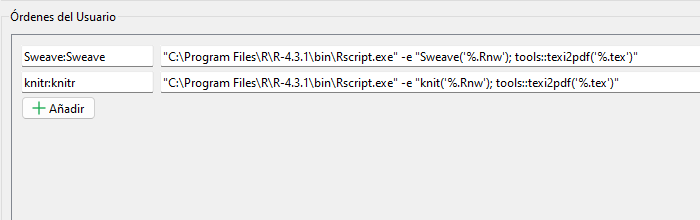
\includegraphics[scale = 0.7]{img/o_usuario}
				\caption{Creación de orden de usuario}
				\label{fig:orden}
			\end{figure}
			
			Ahora basta modificar el botón verde del IDE para que en vez de invocar al compilador \hologo{pdfLaTeX}, lleve a cabo la instrucción que le hemos dado. Para ello volveremos al menú de compilación en el que nos ubicábamos previamente, y observaremos la sección de \textit{Meta-Órdenes}. Modificaremos el valor del campo \textit{Compilador por defecto}, escribiendo \texttt{txs:///knitr} para que se ejecute la orden que previamente hemos creado, o podemos hacerlo de manera gráfica como se observa en la \Cref{fig:comp}. Ahora bastará pulsar el botón verde o F5 para ver a nuestra izquierda el código de nuestro documento, y a la derecha actualizado, el documento PDF final. 
			
			\begin{figure}[H]
				\centering
				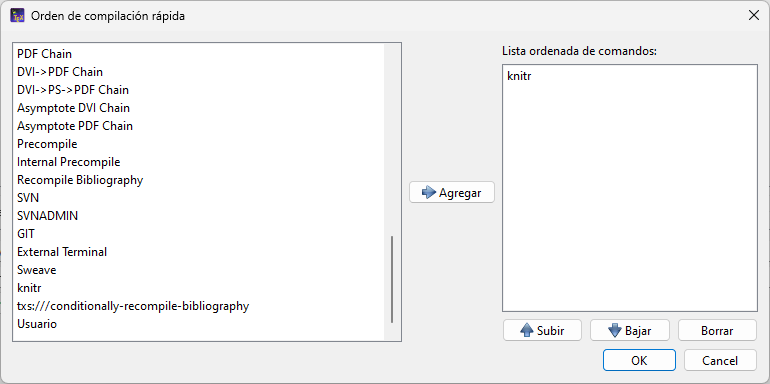
\includegraphics[scale = 0.7]{img/compilacion}
				\caption{Modificación de compilación}
				\label{fig:comp}
			\end{figure}
			
			Por último, para llevar un mejor control de versiones del proyecto, y de coordinación entre los miembros del grupo, se usará un repositorio de GitHub. Añadiremos un archivo \texttt{.gitignore} para no cargar en el repositorio los archivos temporales generados durante la compilación. Otra alternativa que se podría haber usado, es usar Overleaf (aquí usaríamos la extensión \texttt{.Rtex} en vez de \texttt{.Rnw}), ya que no sería necesaria la instalación de ningún software, y también trabaja con Knitr. Sin embargo, la integración de GitHub en Overleaf es de pago, por lo que optamos por usar la configuración explicada hasta el momento, para poder tener un mejor control de versiones sin coste alguno. \\
			
			Por último, mencionar que al igual que R posee su repositorio de paquetes (que ya hemos visto que incluye más cosas) llamado CRAN, \LaTeX{} que en realidad es ``un subconjunto'' del lenguaje \TeX{}, también tiene su propio portal llamado CTAN o Comprehensive \TeX{} Archive Network (\url{https://www.ctan.org/}) de donde se descargan los paquetes y otros materiales para el lenguaje. 
			
			\begin{figure}[H]
				\centering
				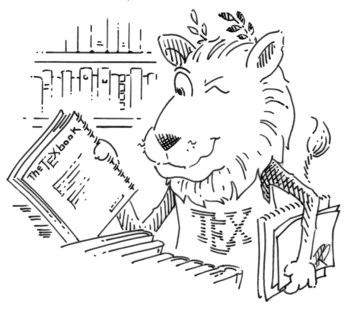
\includegraphics[scale = 0.5]{img/ctan_lion}
				\caption{Mascota de \TeX{} y el CTAN}
				\label{fig:leon}
			\end{figure}
			
	\chapter{Ejercicios guiados}\pagestyle{fancy}
	
		En esta primera parte de esta práctica, repetirán los ejercicios explicados y realizados por el profesor en las clases de laboratorio, utilizando los mismos procedimientos vistos plasmándolos en este documento. 
	
		\section{Descripción de los datos}
		
			\begin{exercise}
				El primer conjunto de datos, que se empleará para realizar el análisis de descripción de datos, estará formado por datos de una característica cualitativa, nombre, y otra cuantitativa, radio, de los satélites menores de Urano, es decir, aquellos que tienen un radio menor de 50 Km, dichos datos, los primeros cualitativos nominales, y los segundos cuantitativos continuos, son: (Nombre, radio en Km): Cordelia, 13; Ofelia, 16; Bianca, 22; Crésida, 33; Desdémona, 29; Julieta, 42; Rosalinda, 27; Belinda, 34; Luna-1986U10, 20; Calíbano, 30; Luna-999U1, 20; Luna 1999U2, 15.
			\end{exercise}
			
			Para comenzar con la resolución de este ejercicio, deberemos escribir los datos en un fichero \texttt{.txt}, cumpliendo las siguientes normas: 
			
			\begin{itemize}
				\item Existirá una tabulación entre dato y dato. 
				\item La primera columna numera las filas, y en la primera fila se introduce un espacio y el nombre de las variables. 
				\item Se introducirá un salto de línea en la última fila
				\item Para los números decimales se utilizarán puntos. 
				\item Al escribir nombres, no se deberán introducir espacios. 
			\end{itemize}
			
			Obedeciendo a estas normas, copiamos los datos en un fichero llamado \texttt{satelites.txt}, y lo cargamos en R de la siguiente manera: 
			
\begin{knitrout}
\definecolor{shadecolor}{rgb}{0.969, 0.969, 0.969}\color{fgcolor}\begin{kframe}
\begin{alltt}
\hlstd{s} \hlkwb{<-} \hlkwd{read.table}\hlstd{(}\hlstr{"data/satelites.txt"}\hlstd{)}
\hlkwd{print}\hlstd{(s)}
\end{alltt}
\begin{verbatim}
##          nombre radio
## 1      Cordelia    13
## 2        Ofelia    16
## 3        Bianca    22
## 4       Crésida    33
## 5     Desdémona    29
## 6       Julieta    42
## 7     Rosalinda    27
## 8       Belinda    34
## 9  Luna-1986U10    20
## 10     Calíbano    30
## 11   Luna-999U1    20
## 12  Luna-1999U2    15
\end{verbatim}
\end{kframe}
\end{knitrout}
			
			Ahora en la variable \texttt{s} tenemos un dataframe con los datos de nuestros satélites. En los dataframes se accede por \texttt{[fila, columna]}, y también podemos consultar las dimensiones con la función \texttt{dim}. Sería de esperar que nos dijera que tiene 12 filas (los 12 datos), y 2 columnas (\texttt{nombre} y \texttt{radio}). 
			
\begin{knitrout}
\definecolor{shadecolor}{rgb}{0.969, 0.969, 0.969}\color{fgcolor}\begin{kframe}
\begin{alltt}
\hlkwd{dim}\hlstd{(s)}
\end{alltt}
\begin{verbatim}
## [1] 12  2
\end{verbatim}
\end{kframe}
\end{knitrout}
			
			También podemos ordenar el dataframe, en función de una de las magnitudes (columnas), usando la función \texttt{order} aplicando recursivamente el concepto de acceder por filas y columnas. Veamos un ejemplo, si en \texttt{s} teníamos guardado nuestro dataframe, y queremos ordenar por \texttt{radio}, la manera de hacerlo sería la siguiente: 
			
\begin{knitrout}
\definecolor{shadecolor}{rgb}{0.969, 0.969, 0.969}\color{fgcolor}\begin{kframe}
\begin{alltt}
\hlstd{s_ordered} \hlkwb{<-} \hlstd{s[}\hlkwd{order}\hlstd{(s}\hlopt{$}\hlstd{radio), ]}
\hlkwd{print}\hlstd{(s_ordered)}
\end{alltt}
\begin{verbatim}
##          nombre radio
## 1      Cordelia    13
## 12  Luna-1999U2    15
## 2        Ofelia    16
## 9  Luna-1986U10    20
## 11   Luna-999U1    20
## 3        Bianca    22
## 7     Rosalinda    27
## 5     Desdémona    29
## 10     Calíbano    30
## 4       Crésida    33
## 8       Belinda    34
## 6       Julieta    42
\end{verbatim}
\end{kframe}
\end{knitrout}
			
			Podemos introducir nuevos criterios a la ordenación, como por ejemplo, hacerlo en orden descendente. Para esto usaremos la función \texttt{rev}. 
			
\begin{knitrout}
\definecolor{shadecolor}{rgb}{0.969, 0.969, 0.969}\color{fgcolor}\begin{kframe}
\begin{alltt}
\hlstd{s_ordered_rev} \hlkwb{<-} \hlstd{s[}\hlkwd{rev}\hlstd{(}\hlkwd{order}\hlstd{(s}\hlopt{$}\hlstd{radio)), ]}
\hlkwd{print}\hlstd{(s_ordered_rev)}
\end{alltt}
\begin{verbatim}
##          nombre radio
## 6       Julieta    42
## 8       Belinda    34
## 4       Crésida    33
## 10     Calíbano    30
## 5     Desdémona    29
## 7     Rosalinda    27
## 3        Bianca    22
## 11   Luna-999U1    20
## 9  Luna-1986U10    20
## 2        Ofelia    16
## 12  Luna-1999U2    15
## 1      Cordelia    13
\end{verbatim}
\end{kframe}
\end{knitrout}
			
			También suele ser útil conocer cuántos elementos tiene una columna. Podemos averiguarlo con la función \texttt{length}, veamos un ejemplo. 
			
\begin{knitrout}
\definecolor{shadecolor}{rgb}{0.969, 0.969, 0.969}\color{fgcolor}\begin{kframe}
\begin{alltt}
\hlkwd{length}\hlstd{(s}\hlopt{$}\hlstd{radio)}
\end{alltt}
\begin{verbatim}
## [1] 12
\end{verbatim}
\end{kframe}
\end{knitrout}
			
			Otro valor que nos podemos plantear calcular es el rango. Para ello podemos usar las funciones \texttt{max} y \texttt{min}. Debemos tener cuidado con la función \texttt{range} y no confundirnos, pues nos dará los valores máximo y mínimo. 
			
\begin{knitrout}
\definecolor{shadecolor}{rgb}{0.969, 0.969, 0.969}\color{fgcolor}\begin{kframe}
\begin{alltt}
\hlstd{r} \hlkwb{<-} \hlkwd{max}\hlstd{(s}\hlopt{$}\hlstd{radio)} \hlopt{-} \hlkwd{min}\hlstd{(s}\hlopt{$}\hlstd{radio)}
\hlkwd{print}\hlstd{(r)}
\end{alltt}
\begin{verbatim}
## [1] 29
\end{verbatim}
\begin{alltt}
\hlkwd{range}\hlstd{(s}\hlopt{$}\hlstd{radio)}
\end{alltt}
\begin{verbatim}
## [1] 13 42
\end{verbatim}
\end{kframe}
\end{knitrout}
			
			Para una mejor lectura, podemos cambiar la forma de obtener la columna de los radios: 
			
\begin{knitrout}
\definecolor{shadecolor}{rgb}{0.969, 0.969, 0.969}\color{fgcolor}\begin{kframe}
\begin{alltt}
\hlstd{radio} \hlkwb{<-} \hlstd{s}\hlopt{$}\hlstd{radio}
\end{alltt}
\end{kframe}
\end{knitrout}
			
			La idea de calcular la diferencia de el máximo y el mínimo a mano parece funcionar, sin embargo, para futuros casos sería más ágil tener codificada una función como la siguiente. 
			
\begin{knitrout}
\definecolor{shadecolor}{rgb}{0.969, 0.969, 0.969}\color{fgcolor}\begin{kframe}
\begin{alltt}
\hlstd{rango} \hlkwb{<-} \hlkwa{function}\hlstd{(}\hlkwc{radio}\hlstd{)\{}\hlkwd{max}\hlstd{(radio)} \hlopt{-} \hlkwd{min}\hlstd{(radio)\}}
\hlkwd{rango}\hlstd{(radio)}
\end{alltt}
\begin{verbatim}
## [1] 29
\end{verbatim}
\end{kframe}
\end{knitrout}
			
			Sin embargo, al salir de R, la definición de la función se pierde, por lo que deberemos guardarla en un fichero, y posteriormente cargarlo en futuras ejecuciones. Lo haremos de la siguiente manera: 
			
\begin{knitrout}
\definecolor{shadecolor}{rgb}{0.969, 0.969, 0.969}\color{fgcolor}\begin{kframe}
\begin{alltt}
\hlkwd{dump}\hlstd{(}\hlstr{"rango"}\hlstd{,} \hlkwc{file} \hlstd{=} \hlstr{"fn/rango.R"}\hlstd{)}
\hlkwd{source}\hlstd{(}\hlstr{"fn/rango.R"}\hlstd{)}
\end{alltt}
\end{kframe}
\end{knitrout}
			
			Volviendo al estudio de nuestros datos, veamos cómo calcular las diferentes frecuencias. Como en R no existe una función para las frecuencias relativas, se definirá y guardará una propia. 
			
			{\small
\begin{knitrout}
\definecolor{shadecolor}{rgb}{0.969, 0.969, 0.969}\color{fgcolor}\begin{kframe}
\begin{alltt}
\hlstd{fabs_radio} \hlkwb{<-} \hlkwd{table}\hlstd{(radio)}
\hlstd{fabsacum_radio} \hlkwb{<-} \hlkwd{cumsum}\hlstd{(fabs_radio)}
\hlstd{frecrel} \hlkwb{<-} \hlkwa{function}\hlstd{(}\hlkwc{r}\hlstd{)\{}\hlkwd{table}\hlstd{(r)}\hlopt{/}\hlkwd{length}\hlstd{(r)\}}
\hlkwd{dump}\hlstd{(}\hlstr{"frecrel"}\hlstd{,} \hlkwc{file} \hlstd{=} \hlstr{"fn/frecrel.R"}\hlstd{)}

\hlkwd{print}\hlstd{(fabs_radio)}
\end{alltt}
\begin{verbatim}
## radio
## 13 15 16 20 22 27 29 30 33 34 42 
##  1  1  1  2  1  1  1  1  1  1  1
\end{verbatim}
\begin{alltt}
\hlkwd{print}\hlstd{(fabsacum_radio)}
\end{alltt}
\begin{verbatim}
## 13 15 16 20 22 27 29 30 33 34 42 
##  1  2  3  5  6  7  8  9 10 11 12
\end{verbatim}
\begin{alltt}
\hlkwd{print}\hlstd{(}\hlkwd{frecrel}\hlstd{(radio))}
\end{alltt}
\begin{verbatim}
## r
##         13         15         16         20         22         27         29 
## 0.08333333 0.08333333 0.08333333 0.16666667 0.08333333 0.08333333 0.08333333 
##         30         33         34         42 
## 0.08333333 0.08333333 0.08333333 0.08333333
\end{verbatim}
\end{kframe}
\end{knitrout}
			}
			
			Otro valor que podemos calcular es la media aritmética de los datos, para ello se cuenta con la función \texttt{mean}. 
			
\begin{knitrout}
\definecolor{shadecolor}{rgb}{0.969, 0.969, 0.969}\color{fgcolor}\begin{kframe}
\begin{alltt}
\hlstd{mr} \hlkwb{<-} \hlkwd{mean}\hlstd{(radio)}
\hlkwd{print}\hlstd{(mr)}
\end{alltt}
\begin{verbatim}
## [1] 25.08333
\end{verbatim}
\end{kframe}
\end{knitrout}
			
			Ahora calcularemos la desviación típica, para ello se cuenta con la función \texttt{sd}. 
			
\begin{knitrout}
\definecolor{shadecolor}{rgb}{0.969, 0.969, 0.969}\color{fgcolor}\begin{kframe}
\begin{alltt}
\hlstd{sdr} \hlkwb{<-} \hlkwd{sd}\hlstd{(radio)}
\hlkwd{print}\hlstd{(sdr)}
\end{alltt}
\begin{verbatim}
## [1] 8.857029
\end{verbatim}
\end{kframe}
\end{knitrout}
			
			Sin embargo, el resultado obtenido no es el esperado. Esto se debe a que esta función realiza el siguiente cálculo
			$$
			s = \sqrt{\frac{\displaystyle\sum_{i=0}^n (x_i-\bar{x})^2}{n-1}}
			$$
			que es más utilizado en inferencia estadística, porque hace que se parezca más a una campana de Gauss (menos sesgo), mientras que la fórmula vista en clase utiliza un factor de $n$ en vez de $n-1$ en el denominador (dentro de la raíz). Para ello, el profesor lo corrigió de la siguiente manera: 
			
\begin{knitrout}
\definecolor{shadecolor}{rgb}{0.969, 0.969, 0.969}\color{fgcolor}\begin{kframe}
\begin{alltt}
\hlstd{sdr2} \hlkwb{<-} \hlkwd{sqrt}\hlstd{((sdr}\hlopt{^}\hlnum{2}\hlstd{)}\hlopt{*}\hlstd{(}\hlkwd{length}\hlstd{(radio)}\hlopt{-}\hlnum{1}\hlstd{)}\hlopt{/}\hlkwd{length}\hlstd{(radio))}
\hlkwd{print}\hlstd{(sdr2)}
\end{alltt}
\begin{verbatim}
## [1] 8.47996
\end{verbatim}
\end{kframe}
\end{knitrout}
			
			En realidad lo que se está realizando es el siguiente ``ajuste'': 
			$$
			s' = \sqrt{s^2\cdot\frac{n-1}{n}}
			$$
			
			Una vez hemos visto cómo se calcula la desviación típica, podremos ver cómo calcular la varianza. Como sabemos que es el cuadrado de la desviación típica, bastaría con elevar al cuadrado si no fuera por el ``fallo'' de $n-1$ visto previamente. En este caso, el profesor lo arregló para el caso particular de la siguiente manera: 
			
\begin{knitrout}
\definecolor{shadecolor}{rgb}{0.969, 0.969, 0.969}\color{fgcolor}\begin{kframe}
\begin{alltt}
\hlstd{varr} \hlkwb{<-} \hlkwd{var}\hlstd{(radio)}
\hlstd{varr} \hlkwb{<-} \hlnum{11}\hlopt{/}\hlnum{12} \hlopt{*} \hlstd{varr}
\hlkwd{print}\hlstd{(varr)}
\end{alltt}
\begin{verbatim}
## [1] 71.90972
\end{verbatim}
\end{kframe}
\end{knitrout}
			
			Otro de los valores que se ha enseñado cómo calcular, es la mediana. Para este caso existe la función \texttt{median}. 
			
\begin{knitrout}
\definecolor{shadecolor}{rgb}{0.969, 0.969, 0.969}\color{fgcolor}\begin{kframe}
\begin{alltt}
\hlstd{medianr} \hlkwb{<-} \hlkwd{median}\hlstd{(radio)}
\hlkwd{print}\hlstd{(medianr)}
\end{alltt}
\begin{verbatim}
## [1] 24.5
\end{verbatim}
\end{kframe}
\end{knitrout}
			
			En último lugar, el profesor enseñó cómo calcular cuantiles, y para ello mostró la función \texttt{quantile}, pero se mencionó que se obtienen resultados diferentes a los esperados debido a la forma que tiene de calcularlos, y se deberá programar. Aquí se muestra un ejemplo de cómo se calcularía el primer cuartil. 
			
\begin{knitrout}
\definecolor{shadecolor}{rgb}{0.969, 0.969, 0.969}\color{fgcolor}\begin{kframe}
\begin{alltt}
\hlstd{cuar1} \hlkwb{<-} \hlkwd{quantile}\hlstd{(radio,} \hlnum{0.25}\hlstd{)}
\hlkwd{print}\hlstd{(cuar1)}
\end{alltt}
\begin{verbatim}
## 25% 
##  19
\end{verbatim}
\end{kframe}
\end{knitrout}
			
			Como añadido, el profesor explicó cómo abrir un ejemplo de Sweave, cómo pasarlo a un fichero que \LaTeX{} pudiese leer, y cómo compilarlo a PDF. Las instrucciones son las que se verán a continuación, aunque como ya se explicó en la introducción, usaremos otra forma de trabajar con estos archivos a lo largo de la práctica. 
			
			\begin{verbatim}
				rnwfile<-system.file("Sweave", "example-1.Rnw", package="utils")
				Sweave(rnwfile)
				tools::texi2pdf("example-1.tex")
			\end{verbatim}
		
		\section{Asociación}
		
			\begin{exercise}
				El segundo conjunto de datos, que se empleará para realizar el análisis de asociación, estará formado por las siguientes 6 cestas de la compra: \{Pan, Agua, Leche, Naranjas\}, \{Pan, Agua, Café, Leche\}, \{Pan, Agua, Leche\}, \{Pan, Café, Leche\}, \{Pan, Agua\}, \{Leche\}.
			\end{exercise}
				
			Lo primero explicado por el profesor fue la preparación de los datos proporcionados para que \texttt{arules} fuese capaz de tratar con ellos. Para ello se introduce una matriz de ceros y unos mediante el paquete \texttt{Matrix}, que indique en cada suceso, qué elementos contiene. La matriz es la siguiente:
			
			$$
			\begin{pmatrix}
				1 & 1 & 0 & 1 & 1\\
				1 & 1 & 1 & 1 & 0\\
				1 & 1 & 0 & 1 & 0\\
				1 & 0 & 1 & 1 & 0\\
				1 & 1 & 0 & 0 & 0\\
				0 & 0 & 0 & 1 & 0
			\end{pmatrix}
			$$
			
			Además, deberemos indicar las dimensiones de esta matriz $(6\times5)$, que estamos introduciendo los datos por filas (\texttt{byrow=TRUE}), y con \texttt{dimnames} ponemos los nombres a las filas y las columnas. El código es el siguiente. 
			
\begin{knitrout}
\definecolor{shadecolor}{rgb}{0.969, 0.969, 0.969}\color{fgcolor}\begin{kframe}
\begin{alltt}
\hlstd{muestra} \hlkwb{<-} \hlkwd{Matrix}\hlstd{(}\hlkwd{c}\hlstd{(}\hlnum{1}\hlstd{,} \hlnum{1}\hlstd{,} \hlnum{0}\hlstd{,} \hlnum{1}\hlstd{,} \hlnum{1}\hlstd{,}
\hlnum{1}\hlstd{,} \hlnum{1}\hlstd{,} \hlnum{1}\hlstd{,} \hlnum{1}\hlstd{,} \hlnum{0}\hlstd{,}
\hlnum{1}\hlstd{,} \hlnum{1}\hlstd{,} \hlnum{0}\hlstd{,} \hlnum{1}\hlstd{,} \hlnum{0}\hlstd{,}
\hlnum{1}\hlstd{,} \hlnum{0}\hlstd{,} \hlnum{1}\hlstd{,} \hlnum{1}\hlstd{,} \hlnum{0}\hlstd{,}
\hlnum{1}\hlstd{,} \hlnum{1}\hlstd{,} \hlnum{0}\hlstd{,} \hlnum{0}\hlstd{,} \hlnum{0}\hlstd{,}
\hlnum{0}\hlstd{,} \hlnum{0}\hlstd{,} \hlnum{0}\hlstd{,} \hlnum{1}\hlstd{,} \hlnum{0}\hlstd{),} \hlnum{6}\hlstd{,} \hlnum{5}\hlstd{,} \hlkwc{byrow} \hlstd{=} \hlnum{TRUE}\hlstd{,} \hlkwc{dimnames} \hlstd{=} \hlkwd{list}\hlstd{(}
\hlkwd{c}\hlstd{(}\hlstr{"suceso1"}\hlstd{,} \hlstr{"suceso2"}\hlstd{,} \hlstr{"suceso3"}\hlstd{,} \hlstr{"suceso4"}\hlstd{,} \hlstr{"suceso5"}\hlstd{,} \hlstr{"suceso6"}\hlstd{),}
\hlkwd{c}\hlstd{(}\hlstr{"Pan"}\hlstd{,} \hlstr{"Agua"}\hlstd{,} \hlstr{"Café"}\hlstd{,} \hlstr{"Leche"}\hlstd{,} \hlstr{"Naranjas"}\hlstd{)),} \hlkwc{sparse}\hlstd{=}\hlnum{TRUE}\hlstd{)}
\hlstd{muestra}
\end{alltt}
\begin{verbatim}
## 6 x 5 sparse Matrix of class "dgCMatrix"
##         Pan Agua Café Leche Naranjas
## suceso1   1    1    .     1        1
## suceso2   1    1    1     1        .
## suceso3   1    1    .     1        .
## suceso4   1    .    1     1        .
## suceso5   1    1    .     .        .
## suceso6   .    .    .     1        .
\end{verbatim}
\end{kframe}
\end{knitrout}
			
			A continuación, se ha enseñado cómo mostrar la matriz con puntos y barras, en vez de con unos y ceros. Se consigue con la función \texttt{as} y el parámetro \texttt{nsparseMatrix}. 
			
\begin{knitrout}
\definecolor{shadecolor}{rgb}{0.969, 0.969, 0.969}\color{fgcolor}\begin{kframe}
\begin{alltt}
\hlstd{muestrangCMatrix} \hlkwb{<-} \hlkwd{as}\hlstd{(muestra,} \hlstr{"nsparseMatrix"}\hlstd{)}
\hlstd{muestrangCMatrix}
\end{alltt}
\begin{verbatim}
## 6 x 5 sparse Matrix of class "ngCMatrix"
##         Pan Agua Café Leche Naranjas
## suceso1   |    |    .     |        |
## suceso2   |    |    |     |        .
## suceso3   |    |    .     |        .
## suceso4   |    .    |     |        .
## suceso5   |    |    .     .        .
## suceso6   .    .    .     |        .
\end{verbatim}
\end{kframe}
\end{knitrout}
			
			Sin embargo, para el algoritmo debemos pasarle justo la transpuesta de la matriz con la que trabajamos, por ello se utiliza la función \texttt{t}. 
			
\begin{knitrout}
\definecolor{shadecolor}{rgb}{0.969, 0.969, 0.969}\color{fgcolor}\begin{kframe}
\begin{alltt}
\hlstd{transpmuestrangCMatrix} \hlkwb{<-} \hlkwd{t}\hlstd{(muestrangCMatrix)}
\hlstd{transpmuestrangCMatrix}
\end{alltt}
\begin{verbatim}
## 5 x 6 sparse Matrix of class "ngCMatrix"
##          suceso1 suceso2 suceso3 suceso4 suceso5 suceso6
## Pan            |       |       |       |       |       .
## Agua           |       |       |       .       |       .
## Café           .       |       .       |       .       .
## Leche          |       |       |       |       .       |
## Naranjas       |       .       .       .       .       .
\end{verbatim}
\end{kframe}
\end{knitrout}
			
			Podemos consultar algunos datos acerca de los datos de nuestra matriz podemos usar la función \texttt{as} con el parámetro \texttt{transactions}. Además, con \texttt{summary} podemos ver un resumen de algunos parámetros básicos de los datos que contiene la matriz. 
			
\begin{knitrout}
\definecolor{shadecolor}{rgb}{0.969, 0.969, 0.969}\color{fgcolor}\begin{kframe}
\begin{alltt}
\hlstd{transacciones} \hlkwb{=} \hlkwd{as}\hlstd{(transpmuestrangCMatrix,} \hlstr{"transactions"}\hlstd{)}
\hlstd{transacciones}
\end{alltt}
\begin{verbatim}
## transactions in sparse format with
##  6 transactions (rows) and
##  5 items (columns)
\end{verbatim}
\begin{alltt}
\hlkwd{summary}\hlstd{(transacciones)}
\end{alltt}
\begin{verbatim}
## transactions as itemMatrix in sparse format with
##  6 rows (elements/itemsets/transactions) and
##  5 columns (items) and a density of 0.5666667 
## 
## most frequent items:
##      Pan    Leche     Agua     Café Naranjas  (Other) 
##        5        5        4        2        1        0 
## 
## element (itemset/transaction) length distribution:
## sizes
## 1 2 3 4 
## 1 1 2 2 
## 
##    Min. 1st Qu.  Median    Mean 3rd Qu.    Max. 
##   1.000   2.250   3.000   2.833   3.750   4.000 
## 
## includes extended item information - examples:
##   labels
## 1    Pan
## 2   Agua
## 3   Café
## 
## includes extended transaction information - examples:
##   itemsetID
## 1   suceso1
## 2   suceso2
## 3   suceso3
\end{verbatim}
\end{kframe}
\end{knitrout}
			
			Finalmente, podemos ejecutar el algoritmo apriori llamando a la función \texttt{apriori} del paquete \texttt{arules}. Definimos el soporte con un valor del 50\%, y la confianza con 80\%. 
			
\begin{knitrout}
\definecolor{shadecolor}{rgb}{0.969, 0.969, 0.969}\color{fgcolor}\begin{kframe}
\begin{alltt}
\hlstd{asociaciones} \hlkwb{=} \hlkwd{apriori}\hlstd{(transacciones,} \hlkwc{parameter} \hlstd{=}
\hlkwd{list}\hlstd{(}\hlkwc{support} \hlstd{=} \hlnum{0.5}\hlstd{,} \hlkwc{confidence} \hlstd{=} \hlnum{0.8}\hlstd{))}
\end{alltt}
\begin{verbatim}
## Apriori
## 
## Parameter specification:
##  confidence minval smax arem  aval originalSupport maxtime support minlen
##         0.8    0.1    1 none FALSE            TRUE       5     0.5      1
##  maxlen target  ext
##      10  rules TRUE
## 
## Algorithmic control:
##  filter tree heap memopt load sort verbose
##     0.1 TRUE TRUE  FALSE TRUE    2    TRUE
## 
## Absolute minimum support count: 3 
## 
## set item appearances ...[0 item(s)] done [0.00s].
## set transactions ...[5 item(s), 6 transaction(s)] done [0.00s].
## sorting and recoding items ... [3 item(s)] done [0.00s].
## creating transaction tree ... done [0.00s].
## checking subsets of size 1 2 3 done [0.00s].
## writing ... [7 rule(s)] done [0.00s].
## creating S4 object  ... done [0.00s].
\end{verbatim}
\end{kframe}
\end{knitrout}
			
			Podemos ver el resultado del algoritmo con la función \texttt{inspect}. 
			
\begin{knitrout}
\definecolor{shadecolor}{rgb}{0.969, 0.969, 0.969}\color{fgcolor}\begin{kframe}
\begin{alltt}
\hlkwd{inspect}\hlstd{(asociaciones)}
\end{alltt}
\begin{verbatim}
##     lhs              rhs     support   confidence coverage  lift count
## [1] {}            => {Leche} 0.8333333 0.8333333  1.0000000 1.00 5    
## [2] {}            => {Pan}   0.8333333 0.8333333  1.0000000 1.00 5    
## [3] {Agua}        => {Pan}   0.6666667 1.0000000  0.6666667 1.20 4    
## [4] {Pan}         => {Agua}  0.6666667 0.8000000  0.8333333 1.20 4    
## [5] {Leche}       => {Pan}   0.6666667 0.8000000  0.8333333 0.96 4    
## [6] {Pan}         => {Leche} 0.6666667 0.8000000  0.8333333 0.96 4    
## [7] {Agua, Leche} => {Pan}   0.5000000 1.0000000  0.5000000 1.20 3
\end{verbatim}
\end{kframe}
\end{knitrout}
			
			Aquí observamos el resultado del algoritmo. Debemos ignorar las dos primeras filas, pues no tiene sentido alguno que $\varnothing \rightarrow$ \{Leche\}, o que $\varnothing \rightarrow$ \{Pan\}, aparecen por cómo el autor del paquete codificó el algoritmo. En el resto de casos $A \rightarrow B$, nos indica cómo de probable es comprar $B$ cuando se compra $A$ (en función del soporte y la confianza provistas). 
			
			
		\section{Detección de datos anómalos}
			
			\subsection{Técnicas estadísticas}
			
				\begin{exercise}
					El tercer conjunto de datos, que se empleará para realizar el análisis de detección de datos anómalos utilizando técnicas con base estadística, estará formado por los siguientes 7 valores de resistencia y densidad para diferentes tipos de hormigón \{Resistencia, Densidad\}: \{3, 2; 3.5, 12; 4.7, 4.1; 5.2, 4.9; 7.1, 6.1; 6.2, 5.2; 14, 5.3\}. Aplicar las medidas de ordenación a la resistencia y las de dispersión a la densidad.
				\end{exercise}
				
				\subsubsection{Caja y bigotes}\label{subsub:caja_bigotes}
				
					Es una herramienta gráfica utilizada en estadística para representar la distribución de un conjunto de datos y detectar sucesos anómalos o outliers. Para realizar el cálculo de los outliers en clase, se introdujeron los datos en una matriz mediante \texttt{matrix}, luego se transpuso y se pasó a un \texttt{dataframe}. Para esta primera técnica vamos a usar la primera columna (\texttt{resistencia}).
					
\begin{knitrout}
\definecolor{shadecolor}{rgb}{0.969, 0.969, 0.969}\color{fgcolor}\begin{kframe}
\begin{alltt}
\hlstd{muestra}\hlkwb{=}\hlkwd{t}\hlstd{(}\hlkwd{matrix}\hlstd{(}\hlkwd{c}\hlstd{(}\hlnum{3}\hlstd{,}\hlnum{2}\hlstd{,}\hlnum{3.5}\hlstd{,}\hlnum{12}\hlstd{,}\hlnum{4.7}\hlstd{,}\hlnum{4.1}\hlstd{,}\hlnum{5.2}\hlstd{,}\hlnum{4.9}\hlstd{,}\hlnum{7.1}\hlstd{,}\hlnum{6.1}\hlstd{,}\hlnum{6.2}\hlstd{,}\hlnum{5.2}\hlstd{,}\hlnum{14}\hlstd{,}\hlnum{5.3}\hlstd{),}
\hlnum{2}\hlstd{,}\hlnum{7}\hlstd{,}\hlkwc{dimnames}\hlstd{=}\hlkwd{list}\hlstd{(}\hlkwd{c}\hlstd{(}\hlstr{"resistencia"}\hlstd{,}\hlstr{"densidad"}\hlstd{))))}

\hlstd{(muestra}\hlkwb{=}\hlkwd{data.frame}\hlstd{(muestra))}
\end{alltt}
\begin{verbatim}
##   resistencia densidad
## 1         3.0      2.0
## 2         3.5     12.0
## 3         4.7      4.1
## 4         5.2      4.9
## 5         7.1      6.1
## 6         6.2      5.2
## 7        14.0      5.3
\end{verbatim}
\end{kframe}
\end{knitrout}
					
					Una forma de obtener los outliers es mediante la función \texttt{boxplot}, pasándole la columna de los datos, el grado de outlier (\texttt{range}) o distancia a la que el suceso se considera outlier, y por último \texttt{plot=FALSE}, que se usa para no mostrar el gráfico como tal y solo sacar la información por el terminal.
					
\begin{knitrout}
\definecolor{shadecolor}{rgb}{0.969, 0.969, 0.969}\color{fgcolor}\begin{kframe}
\begin{alltt}
\hlstd{(}\hlkwd{boxplot}\hlstd{(muestra}\hlopt{$}\hlstd{r,} \hlkwc{range}\hlstd{=}\hlnum{1.5}\hlstd{,} \hlkwc{plot}\hlstd{=}\hlnum{FALSE}\hlstd{))}
\end{alltt}
\begin{verbatim}
## $stats
##      [,1]
## [1,] 3.00
## [2,] 4.10
## [3,] 5.20
## [4,] 6.65
## [5,] 7.10
## 
## $n
## [1] 7
## 
## $conf
##          [,1]
## [1,] 3.677181
## [2,] 6.722819
## 
## $out
## [1] 14
## 
## $group
## [1] 1
## 
## $names
## [1] "1"
\end{verbatim}
\end{kframe}
\end{knitrout}
					
					Como podemos ver en \texttt{\$out}, se obtiene que el suceso outlier es el 14, que como se vio en el ejercicio de la clase de teoría es correcto, pero, si nos fijamos en \texttt{\$conf}, se pueden ver los límites del intervalo, pero estos no coinciden con los vistos en clase. Esto se debe a que al igual que ocurría al usar la función \texttt{sd} para el cálculo de la desviación, R utiliza un factor de $n-1$ en vez de $n$, por lo que no son los valores exactos. \\
					
					Ahora vamos a hacerlo mediante el cálculo de los cuartiles como se vio en ejercicios anteriores. Además, se han calculado los límites del intervalo mediante la siguiente ecuación.
					
					\begin{equation}
						(Q_1 - d(Q_3 - Q_1), Q_3 + d(Q_3 - Q_1))
						\label{eq:intervalo_cuart}
					\end{equation}
					
\begin{knitrout}
\definecolor{shadecolor}{rgb}{0.969, 0.969, 0.969}\color{fgcolor}\begin{kframe}
\begin{alltt}
\hlstd{(cuar1r}\hlkwb{=}\hlkwd{quantile}\hlstd{(muestra}\hlopt{$}\hlstd{r,} \hlnum{0.25}\hlstd{))}
\end{alltt}
\begin{verbatim}
## 25% 
## 4.1
\end{verbatim}
\begin{alltt}
\hlstd{(cuar3r}\hlkwb{=}\hlkwd{quantile}\hlstd{(muestra}\hlopt{$}\hlstd{r,} \hlnum{0.75}\hlstd{))}
\end{alltt}
\begin{verbatim}
##  75% 
## 6.65
\end{verbatim}
\begin{alltt}
\hlstd{(int}\hlkwb{=}\hlkwd{c}\hlstd{(cuar1r}\hlopt{-}\hlnum{1.5}\hlopt{*}\hlstd{(cuar3r}\hlopt{-}\hlstd{cuar1r), cuar3r}\hlopt{+}\hlnum{1.5}\hlopt{*}\hlstd{(cuar3r}\hlopt{-}\hlstd{cuar1r)))}
\end{alltt}
\begin{verbatim}
##    25%    75% 
##  0.275 10.475
\end{verbatim}
\end{kframe}
\end{knitrout}
					
					Por último, se iteran los elementos de la muestra y se comprueba para cada uno si es menor que el límite inferior del intervalo o si es mayor que el límite superior.
					
\begin{knitrout}
\definecolor{shadecolor}{rgb}{0.969, 0.969, 0.969}\color{fgcolor}\begin{kframe}
\begin{alltt}
\hlkwa{for} \hlstd{(i} \hlkwa{in} \hlnum{1}\hlopt{:}\hlkwd{length}\hlstd{(muestra}\hlopt{$}\hlstd{r)) \{}
        \hlkwa{if} \hlstd{(muestra}\hlopt{$}\hlstd{r[i]} \hlopt{<} \hlstd{int[}\hlnum{1}\hlstd{]} \hlopt{||} \hlstd{muestra}\hlopt{$}\hlstd{r[i]} \hlopt{>} \hlstd{int[}\hlnum{2}\hlstd{]) \{}
                \hlkwd{print}\hlstd{(}\hlstr{"el suceso"}\hlstd{)}
                \hlkwd{print}\hlstd{(i)}
                \hlkwd{print}\hlstd{(}\hlstr{"es un suceso anómalo o outlier"}\hlstd{)}
        \hlstd{\}}
\hlstd{\}}
\end{alltt}
\begin{verbatim}
## [1] "el suceso"
## [1] 7
## [1] "es un suceso anómalo o outlier"
\end{verbatim}
\end{kframe}
\end{knitrout}
					
					En este ejercicio, al igual que se vio en clase, el suceso outlier es el que está en la posición número 7, es decir el elemento 14.
				
				\subsubsection{Media y desviación}
				
					Otra manera de buscar sucesos outliers usando técnicas con base estadística es mediante el uso de la media y la desviación típica. Aquí vamos a usar la otra columna del dataframe (\texttt{densidad}), mediante el uso de las funciones \texttt{mean} y \texttt{sd} sacamos ambos valores, que unimos en los límites del intervalo mediante la siguiente ecuación.
					
					\begin{equation}
						(\bar{x}_a - d\cdot s_a, \bar{x}_a + d\cdot s_a)
						\label{eq:intervalo_xd}
					\end{equation}
					
\begin{knitrout}
\definecolor{shadecolor}{rgb}{0.969, 0.969, 0.969}\color{fgcolor}\begin{kframe}
\begin{alltt}
\hlstd{(media} \hlkwb{=} \hlkwd{mean}\hlstd{(muestra}\hlopt{$}\hlstd{d))}
\end{alltt}
\begin{verbatim}
## [1] 5.657143
\end{verbatim}
\begin{alltt}
\hlstd{(desv} \hlkwb{=} \hlkwd{sd}\hlstd{(muestra}\hlopt{$}\hlstd{d))}
\end{alltt}
\begin{verbatim}
## [1] 3.085913
\end{verbatim}
\begin{alltt}
\hlstd{(int}\hlkwb{=}\hlkwd{c}\hlstd{(media}\hlopt{-}\hlnum{2}\hlopt{*}\hlstd{desv, media}\hlopt{+}\hlnum{2}\hlopt{*}\hlstd{desv))}
\end{alltt}
\begin{verbatim}
## [1] -0.5146825 11.8289682
\end{verbatim}
\end{kframe}
\end{knitrout}
					
					Se puede ver que los valores inferior y superior del intervalo no son iguales que en el ejercicio que realizado en clase, esto se debe a que, como ya se vio, la desviación típica se calcula con un factor de $n-1$ en vez de $n$, por lo que arreglando el cálculo de la desviación quedaría así.
					
\begin{knitrout}
\definecolor{shadecolor}{rgb}{0.969, 0.969, 0.969}\color{fgcolor}\begin{kframe}
\begin{alltt}
\hlstd{(desv} \hlkwb{=} \hlkwd{sqrt}\hlstd{(}\hlkwd{sd}\hlstd{(muestra}\hlopt{$}\hlstd{d)}\hlopt{^}\hlnum{2} \hlopt{*}
\hlstd{(}\hlkwd{length}\hlstd{(muestra}\hlopt{$}\hlstd{d)}\hlopt{-}\hlnum{1}\hlstd{)} \hlopt{/} \hlkwd{length}\hlstd{(muestra}\hlopt{$}\hlstd{d)))}
\end{alltt}
\begin{verbatim}
## [1] 2.857
\end{verbatim}
\begin{alltt}
\hlstd{(int}\hlkwb{=}\hlkwd{c}\hlstd{(media}\hlopt{-}\hlnum{2}\hlopt{*}\hlstd{desv, media}\hlopt{+}\hlnum{2}\hlopt{*}\hlstd{desv))}
\end{alltt}
\begin{verbatim}
## [1] -0.05685714 11.37114285
\end{verbatim}
\begin{alltt}
\hlkwa{for} \hlstd{(i} \hlkwa{in} \hlnum{1}\hlopt{:}\hlkwd{length}\hlstd{(muestra}\hlopt{$}\hlstd{d)) \{}
        \hlkwa{if} \hlstd{(muestra}\hlopt{$}\hlstd{d[i]} \hlopt{<} \hlstd{int[}\hlnum{1}\hlstd{]} \hlopt{||} \hlstd{muestra}\hlopt{$}\hlstd{d[i]} \hlopt{>} \hlstd{int[}\hlnum{2}\hlstd{]) \{}
                \hlkwd{print}\hlstd{(}\hlstr{"el suceso"}\hlstd{)}
                \hlkwd{print}\hlstd{(i)}
                \hlkwd{print}\hlstd{(}\hlstr{"es un suceso anómalo o outlier"}\hlstd{)}
        \hlstd{\}}
\hlstd{\}}
\end{alltt}
\begin{verbatim}
## [1] "el suceso"
## [1] 2
## [1] "es un suceso anómalo o outlier"
\end{verbatim}
\end{kframe}
\end{knitrout}
					
					Como resultado, se obtienen los valores del intervalo correctos y se puede ver que el suceso anómalo es el que se encuentra en la posición 2, es decir el elemento 12.
				
			\subsection{Técnicas de proximidad y densidad}
			
				\begin{exercise}
					El cuarto conjunto de datos, que se empleará para realizar el análisis de detección de datos anómalos utilizando técnicas basadas en la proximidad y en la densidad, estará formado por las siguientes 5 calificaciones de estudiantes: 1. \{4, 4\}; 2. \{4, 3\}; 3. \{5, 5\}; 4. \{1, 1\}; 5. \{5, 4\} donde las características de las calificaciones son: (Teoría, Laboratorio).
				\end{exercise}
				
				\subsubsection{Algoritmo $k-$vecinos}
				
					El algoritmo $k-$vecinos utilizado para identificar outliers basado en distancias, consiste en calcular la distancia de un punto a sus $k$ vecinos más cercanos y considerar los puntos con distancias mayores a un cierto valor (grado de outlier) como anómalos.\\
					
					En clase se añadieron todos los datos de la nueva muestra a una matriz, que luego fue transpuesta para tener los datos dispuestos como requería el cálculo de distancias. Se calcularon las distancias euclídeas mediante la función \texttt{dist} y se guardó en una matriz de $5 \times 5$, para poder visualizar la distancia de cada punto hacia el resto. El cálculo de esta distancia se realiza de la siguiente manera.
					
					$$
					\dt(p, q) = \sqrt{\sum_{i=1}^n(p_i-q_i)^2}
					$$
					
\begin{knitrout}
\definecolor{shadecolor}{rgb}{0.969, 0.969, 0.969}\color{fgcolor}\begin{kframe}
\begin{alltt}
\hlstd{muestra}\hlkwb{=}\hlkwd{matrix}\hlstd{(}\hlkwd{c}\hlstd{(}\hlnum{4}\hlstd{,}\hlnum{4}\hlstd{,}\hlnum{4}\hlstd{,}\hlnum{3}\hlstd{,}\hlnum{5}\hlstd{,}\hlnum{5}\hlstd{,}\hlnum{1}\hlstd{,}\hlnum{1}\hlstd{,}\hlnum{5}\hlstd{,}\hlnum{4}\hlstd{),}\hlnum{2}\hlstd{,}\hlnum{5}\hlstd{)}
\hlstd{muestra}\hlkwb{=}\hlkwd{t}\hlstd{(muestra)}
\hlstd{distancias}\hlkwb{=}\hlkwd{as.matrix}\hlstd{(}\hlkwd{dist}\hlstd{(muestra))}
\hlstd{(distancias}\hlkwb{=}\hlkwd{matrix}\hlstd{(distancias,}\hlnum{5}\hlstd{,}\hlnum{5}\hlstd{))}
\end{alltt}
\begin{verbatim}
##          [,1]     [,2]     [,3]     [,4]     [,5]
## [1,] 0.000000 1.000000 1.414214 4.242641 1.000000
## [2,] 1.000000 0.000000 2.236068 3.605551 1.414214
## [3,] 1.414214 2.236068 0.000000 5.656854 1.000000
## [4,] 4.242641 3.605551 5.656854 0.000000 5.000000
## [5,] 1.000000 1.414214 1.000000 5.000000 0.000000
\end{verbatim}
\end{kframe}
\end{knitrout}
					
					Mediante el siguiente bucle, se itera cada punto y ordena de menor a mayor las distancias hacia los demás puntos.
					
\begin{knitrout}
\definecolor{shadecolor}{rgb}{0.969, 0.969, 0.969}\color{fgcolor}\begin{kframe}
\begin{alltt}
\hlkwa{for} \hlstd{(i} \hlkwa{in} \hlnum{1}\hlopt{:}\hlnum{5}\hlstd{) \{}
        \hlstd{distancias[,i]} \hlkwb{=} \hlkwd{sort}\hlstd{(distancias[,i])}
\hlstd{\}}

\hlstd{(distanciasordenadas}\hlkwb{=}\hlstd{distancias)}
\end{alltt}
\begin{verbatim}
##          [,1]     [,2]     [,3]     [,4]     [,5]
## [1,] 0.000000 0.000000 0.000000 0.000000 0.000000
## [2,] 1.000000 1.000000 1.000000 3.605551 1.000000
## [3,] 1.000000 1.414214 1.414214 4.242641 1.000000
## [4,] 1.414214 2.236068 2.236068 5.000000 1.414214
## [5,] 4.242641 3.605551 5.656854 5.656854 5.000000
\end{verbatim}
\end{kframe}
\end{knitrout}
					
					Por último, se itera cada punto de la matriz de distancias ordenadas y comprobamos si el elemento $k-$éismo está a una distancia mayor de $2.5$ (elegido arbitrariamente), donde el punto se consideraría outlier.\\
					
					En el código se puede ver que se elige el elemento 4 en vez del 3 que era la \texttt{k} elegida para resolverlo, esto se debe a que la primera fila de valores, son las distancias desde cada punto hacia sí mismo, es decir, siempre 0, por lo que los descartamos en el conteo de los \texttt{k} elementos.
					
\begin{knitrout}
\definecolor{shadecolor}{rgb}{0.969, 0.969, 0.969}\color{fgcolor}\begin{kframe}
\begin{alltt}
\hlkwa{for} \hlstd{(i} \hlkwa{in} \hlnum{1}\hlopt{:}\hlnum{5}\hlstd{) \{}
        \hlkwa{if} \hlstd{(distanciasordenadas[}\hlnum{4}\hlstd{,i]} \hlopt{>} \hlnum{2.5}\hlstd{) \{}
                \hlkwd{print}\hlstd{(i)}
                \hlkwd{print}\hlstd{(}\hlstr{"es un suceso anómalo o outlier"}\hlstd{)}
        \hlstd{\}}
\hlstd{\}}
\end{alltt}
\begin{verbatim}
## [1] 4
## [1] "es un suceso anómalo o outlier"
\end{verbatim}
\end{kframe}
\end{knitrout}
					
					Podemos ver que como salida se obtiene que el punto 4 es un suceso anómalo o outlier, al igual que ocurría en el ejercicio resuelto en teoría.
				
				\subsubsection{Algoritmo LOF}
				
					Como último ejercicio realizado en clase, se ha empleado el algoritmo LOF o \textsc{Local Outlier Factor} para identificar outliers basado en distancias, que evalúa la densidad local de puntos en relación con sus vecinos, identificando valores anómalos en regiones menos densas que el entorno circundante.\\
					
					Se obtiene una matriz de distancias haciendo uso de la función \texttt{dist}, pero en este caso se pasa como parámetro el método que queremos que sea usado para calcular la distancia (\texttt{method="manhattan"}), en este caso el método \textit{Manhattan}, que se calcula de la siguiente manera.
					
					$$
					\dt(x_i, x_j) = |x_{i_1} - x_{j_1}| + |x_{i_2} - x_{j_2}|
					$$
					
\begin{knitrout}
\definecolor{shadecolor}{rgb}{0.969, 0.969, 0.969}\color{fgcolor}\begin{kframe}
\begin{alltt}
\hlstd{(distanciasM}\hlkwb{=}\hlkwd{as.matrix}\hlstd{(}\hlkwd{dist}\hlstd{(muestra,} \hlkwc{method}\hlstd{=}\hlstr{"manhattan"}\hlstd{)))}
\end{alltt}
\begin{verbatim}
##   1 2 3 4 5
## 1 0 1 2 6 1
## 2 1 0 3 5 2
## 3 2 3 0 8 1
## 4 6 5 8 0 7
## 5 1 2 1 7 0
\end{verbatim}
\end{kframe}
\end{knitrout}
					
					Para finalizar, el profesor nombró algunos paquetes que realizaban una implementación no simplificada del algoritmo, estos son \texttt{RLof}, \texttt{DDoutlier} y \texttt{DMwR}, pero en el segundo ejercicio autónomo de detección de datos anómalos, se implementará un código propio, que realice las simplificaciones oportunas.
	
	\chapter{Ejercicios autónomos}
	
		\section{Descripción de los datos}\label{sec:descrip_auto}
		
			\begin{exercise}
				El primer conjunto de datos, que se empleará para realizar el análisis de descripción de datos, estará formado por datos de una característica cuantitativa, distancia, desde el domicilio de cada estudiantes hasta la Universidad, dichos datos, cuantitativos continuos, son: 16.5, 34.8, 20.7, 6.2, 4.4, 3.4, 24, 24, 32, 30, 33, 27, 15, 9.4, 2.1, 34, 24, 12, 4.4, 28, 31.4, 21.6, 3.1, 4.5, 5.1, 4, 3.2, 25, 4.5, 20, 34, 12, 12, 12, 12, 5, 19, 30, 5.5, 38, 25, 3.7, 9, 30, 13, 30, 30, 26, 30, 30, 1, 26, 22, 10, 9.7, 11, 24.1, 33, 17.2, 27, 24, 27, 21, 28, 30, 4, 46, 29, 3.7, 2.7, 8.1, 19, 16.
			\end{exercise}
			
			Para comenzar, se han introducido todos los datos en un fichero CSV. Para realizar este fichero se ha abierto un fichero Excel y se han ido introduciendo los datos en la primera columna. Cabe destacar que la primera fila no corresponde a ningún valor ya que se ha puesto \texttt{Distancia} (km) para mantener la estructura con respecto al ejercicio guiado. Una vez han sido introducidos todos los datos, guardamos el fichero con extensión \texttt{.csv}. Para leer este fichero dentro de R se hace uso de la función \texttt{read.csv}, perteneciente al paquete por defecto \texttt{utils}. Esta función en realidad es un uso diferente de la función \texttt{read.table} orientado a la lectura de ficheros CSV. Esta función lee el archivo en formato tabla y a partir de él crea un dataframe haciendo corresponder las filas y las columnas de la tabla.\\
			
			La función empleada ha sido \texttt{read.csv} primeramente porque es un fichero CSV y además porque está delimitado por comas (en caso de haber estado delimitado por punto y coma se debería haber usado \texttt{read.csv2}. Se observa en la siguiente línea de código cómo se ha creado un archivo \texttt{distancia\_universitarios.csv} siguiendo la estructura mencionada previamente. Con este fichero creado basta con llamar a la función \texttt{read.csv} pasando como parámetro el fichero. Si el archivo estuviera en otro directorio, habría que pasar por parámetro la ruta donde se encuentra dicho archivo.
			
\begin{knitrout}
\definecolor{shadecolor}{rgb}{0.969, 0.969, 0.969}\color{fgcolor}\begin{kframe}
\begin{alltt}
\hlstd{fichero} \hlkwb{=} \hlkwd{read.csv}\hlstd{(}\hlstr{"data/distancia_universitarios.csv"}\hlstd{)}
\hlstd{fichero}
\end{alltt}
\begin{verbatim}
##    Distancia
## 1       16.5
## 2       34.8
## 3       20.7
## 4        6.2
## 5        4.4
## 6        3.4
## 7       24.0
## 8       24.0
## 9       32.0
## 10      30.0
## 11      33.0
## 12      27.0
## 13      15.0
## 14       9.4
## 15       2.1
## 16      34.0
## 17      24.0
## 18      12.0
## 19       4.4
## 20      28.0
## 21      31.4
## 22      21.6
## 23       3.1
## 24       4.5
## 25       5.1
## 26       4.0
## 27       3.2
## 28      25.0
## 29       4.5
## 30      20.0
## 31      34.0
## 32      12.0
## 33      12.0
## 34      12.0
## 35      12.0
## 36       5.0
## 37      19.0
## 38      30.0
## 39       5.5
## 40      38.0
## 41      25.0
## 42       3.7
## 43       9.0
## 44      30.0
## 45      13.0
## 46      30.0
## 47      30.0
## 48      26.0
## 49      30.0
## 50      30.0
## 51       1.0
## 52      26.0
## 53      22.0
## 54      10.0
## 55       9.7
## 56      11.0
## 57      24.1
## 58      33.0
## 59      17.2
## 60      27.0
## 61      24.0
## 62      27.0
## 63      21.0
## 64      28.0
## 65      30.0
## 66       4.0
## 67      46.0
## 68      29.0
## 69       3.7
## 70       2.7
## 71       8.1
## 72      19.0
## 73      16.0
\end{verbatim}
\end{kframe}
\end{knitrout}
			
			Como se puede observar, se ha leído correctamente el fichero, creando el dataframe con los datos leídos. Al ser un CSV delimitado por comas, hay que tener cuidado con los números decimales y separar estos por un punto, ya que si se separa por comas, se leerán dos datos en vez de uno.\\ 
			
			Como se va a trabajar todo el rato con la columna \texttt{Distancia} del dataframe, para no tener que acceder repetidamente a esta, podemos definirla en una variable nueva a la que llamaremos \texttt{distancias}, de tal forma que no se tenga que estar pasando \texttt{fichero\$Distancia} repetidamente.
			
\begin{knitrout}
\definecolor{shadecolor}{rgb}{0.969, 0.969, 0.969}\color{fgcolor}\begin{kframe}
\begin{alltt}
\hlstd{distancias} \hlkwb{=} \hlstd{fichero}\hlopt{$}\hlstd{Distancia}
\end{alltt}
\end{kframe}
\end{knitrout}
			
			Para conocer la longitud de \texttt{distancias}, se ha decidido elaborar una función propia, la cual nos devolverá un escalar con el número de elementos que contenga nuestra lista (distancias en este caso). 
			
\begin{knitrout}
\definecolor{shadecolor}{rgb}{0.969, 0.969, 0.969}\color{fgcolor}\begin{kframe}
\begin{alltt}
\hlstd{len} \hlkwb{=} \hlkwa{function}\hlstd{(}\hlkwc{list}\hlstd{) \{}
        \hlstd{count} \hlkwb{=} \hlnum{0}
        \hlkwa{for} \hlstd{(element} \hlkwa{in} \hlstd{list) \{}
                \hlstd{count} \hlkwb{=} \hlstd{count} \hlopt{+} \hlnum{1}
        \hlstd{\}}
        \hlstd{count}
\hlstd{\}}
\end{alltt}
\end{kframe}
\end{knitrout}
			
			La función \texttt{len} se basa en un contador el cual se inicializa a 0 y, por medio de un bucle, iterar todos los elementos de la lista y aumentar en 1 cada vez que haya un nuevo elemento. Por último, se devolverá el contador. Esta función será fundamental en otras funciones tal y como veremos más adelante. Veamos cuántas distancias se tienen:
			
\begin{knitrout}
\definecolor{shadecolor}{rgb}{0.969, 0.969, 0.969}\color{fgcolor}\begin{kframe}
\begin{alltt}
\hlstd{(longitud} \hlkwb{=} \hlkwd{len}\hlstd{(distancias))}
\end{alltt}
\begin{verbatim}
## [1] 73
\end{verbatim}
\end{kframe}
\end{knitrout}
			
			Observamos se tienen 73 elementos, es decir, 73 distancias. La próxima utilidad que se necesita es la ordenación de la lista de distancias. Para ello se ha elaborado una función que ordenará la lista en sentido ascendente o descendente utilizando el método de la burbuja. \\
			
			El método de la burbuja consiste en ir evaluando por pares todos los elementos de una lista, de tal forma que se vayan reposicionando según el sentido en el que se esté ordenando. En caso de ir ordenando en sentido ascendente, el mayor elemento de la lista se irá reposicionando hasta llegar a la derecha del todo. En caso de hacerlo en sentido descendente, el elemento que quedará a la derecha del todo será el menor. Conforme se vaya avanzando, tendremos por cada iteración un elemento más colocado a la derecha del todo, y así sucesivamente hasta que todos los elementos queden ordenados. Esto se consigue en un tiempo $\mathcal{O}(n^2)$. La función que realiza este método de ordenación es la siguiente:
			
\begin{knitrout}
\definecolor{shadecolor}{rgb}{0.969, 0.969, 0.969}\color{fgcolor}\begin{kframe}
\begin{alltt}
\hlstd{bubble} \hlkwb{=} \hlkwa{function}\hlstd{(}\hlkwc{list}\hlstd{,} \hlkwc{asc} \hlstd{=} \hlnum{TRUE}\hlstd{) \{}
        \hlstd{n} \hlkwb{=} \hlkwd{len}\hlstd{(list)}
        \hlstd{direccion} \hlkwb{=} \hlkwd{ifelse}\hlstd{(asc,} \hlnum{1}\hlstd{,} \hlopt{-}\hlnum{1}\hlstd{)}
        \hlkwa{for} \hlstd{(i} \hlkwa{in} \hlnum{2}\hlopt{:}\hlstd{n) \{}
                \hlkwa{for} \hlstd{(j} \hlkwa{in} \hlnum{1}\hlopt{:}\hlstd{(n}\hlopt{-}\hlnum{1}\hlstd{)) \{}
                        \hlkwa{if} \hlstd{(list[j]} \hlopt{*} \hlstd{direccion} \hlopt{>} \hlstd{list[j}\hlopt{+}\hlnum{1}\hlstd{]} \hlopt{*} \hlstd{direccion) \{}
                                \hlstd{temp} \hlkwb{=} \hlstd{list[j]}
                                \hlstd{list[j]} \hlkwb{=} \hlstd{list[j}\hlopt{+}\hlnum{1}\hlstd{]}
                                \hlstd{list[j}\hlopt{+}\hlnum{1}\hlstd{]} \hlkwb{=} \hlstd{temp}
                        \hlstd{\}}
                \hlstd{\}}
        \hlstd{\}}
        \hlstd{list}
\hlstd{\}}
\end{alltt}
\end{kframe}
\end{knitrout}
			
			A esta función se le deberá pasar la lista que se quiere ordenar y \texttt{TRUE} o \texttt{FALSE} para indicar en el sentido que se quiere ordenar. En caso de ser \texttt{TRUE} se ordenará de manera ascendente, y en caso de \texttt{FALSE} se ordenará de forma descendente. Por defecto, si solo se pasa como parámetro la lista, se ordenará de forma ascendente.\\
			
			Además, el algoritmo de ordenación de la burbuja hace uso de la variable \texttt{direccion}, la cual adquiere los valores de 1 (en sentido ascendente) y -1 (en sentido descendente). Esto se consigue con la función \texttt{ifelse} del paquete \texttt{base}, a la cual se le pasa un valor booleano y dos valores. En función del valor booleano, si este es \texttt{TRUE} se coge el primer valor y si es \texttt{FALSE} el segundo. El valor escogido es asignado a la variable \texttt{direccion}. Esta cambiará o no el signo de los elementos de la lista que se está ordenando. En los números positivos, cuanto mayor sea el valor mayor será este, y en los negativos al revés. Si se ordena una lista de números negativos quedará a la derecha del todo el menor valor al ser este el número mayor. Esto se puede generalizar al sentido de ordenación de la lista.\\
			
			Hagamos la prueba con la lista de distancias:
			
			{\small 
\begin{knitrout}
\definecolor{shadecolor}{rgb}{0.969, 0.969, 0.969}\color{fgcolor}\begin{kframe}
\begin{alltt}
\hlstd{distancias_asc} \hlkwb{=} \hlkwd{bubble}\hlstd{(distancias)}
\hlstd{distancias_asc}
\end{alltt}
\begin{verbatim}
##  [1]  1.0  2.1  2.7  3.1  3.2  3.4  3.7  3.7  4.0  4.0  4.4  4.4  4.5  4.5  5.0
## [16]  5.1  5.5  6.2  8.1  9.0  9.4  9.7 10.0 11.0 12.0 12.0 12.0 12.0 12.0 13.0
## [31] 15.0 16.0 16.5 17.2 19.0 19.0 20.0 20.7 21.0 21.6 22.0 24.0 24.0 24.0 24.0
## [46] 24.1 25.0 25.0 26.0 26.0 27.0 27.0 27.0 28.0 28.0 29.0 30.0 30.0 30.0 30.0
## [61] 30.0 30.0 30.0 30.0 31.4 32.0 33.0 33.0 34.0 34.0 34.8 38.0 46.0
\end{verbatim}
\begin{alltt}
\hlstd{distancias_desc} \hlkwb{=} \hlkwd{bubble}\hlstd{(distancias,} \hlnum{FALSE}\hlstd{)}
\hlstd{distancias_desc}
\end{alltt}
\begin{verbatim}
##  [1] 46.0 38.0 34.8 34.0 34.0 33.0 33.0 32.0 31.4 30.0 30.0 30.0 30.0 30.0 30.0
## [16] 30.0 30.0 29.0 28.0 28.0 27.0 27.0 27.0 26.0 26.0 25.0 25.0 24.1 24.0 24.0
## [31] 24.0 24.0 22.0 21.6 21.0 20.7 20.0 19.0 19.0 17.2 16.5 16.0 15.0 13.0 12.0
## [46] 12.0 12.0 12.0 12.0 11.0 10.0  9.7  9.4  9.0  8.1  6.2  5.5  5.1  5.0  4.5
## [61]  4.5  4.4  4.4  4.0  4.0  3.7  3.7  3.4  3.2  3.1  2.7  2.1  1.0
\end{verbatim}
\end{kframe}
\end{knitrout}
			}
			
			Con la lista ordenada, se puede saber de forma muy sencilla el rango. Previamente, en los ejercicios guiados, se tenía que llamar a las funciones \texttt{max} y \texttt{min}. Con la lista ordenada, se pueden acceder a estos valores, ya que estarán en el primer y último índice en función del sentido en el que hayamos ordenado la lista. Es por ello que resulta muy fácil crear una función rango.
			
\begin{knitrout}
\definecolor{shadecolor}{rgb}{0.969, 0.969, 0.969}\color{fgcolor}\begin{kframe}
\begin{alltt}
\hlstd{rank} \hlkwb{=} \hlkwa{function}\hlstd{(}\hlkwc{list}\hlstd{) \{}
        \hlstd{ordered_list} \hlkwb{=} \hlkwd{bubble}\hlstd{(list)}
        \hlstd{ordered_list[}\hlkwd{len}\hlstd{(ordered_list)]} \hlopt{-} \hlstd{ordered_list[}\hlnum{1}\hlstd{]}
\hlstd{\}}
\end{alltt}
\end{kframe}
\end{knitrout}
			
			Primeramente, se ha ordenado la lista en orden ascendente, de tal forma que el valor máximo se encontrará en el último índice y el valor mínimo en el primero. Para calcular el rango se resta al elemento del último índice, el del primero. Se comprueba la función y se observa que se obtiene un rango de 45.
			
\begin{knitrout}
\definecolor{shadecolor}{rgb}{0.969, 0.969, 0.969}\color{fgcolor}\begin{kframe}
\begin{alltt}
\hlstd{rango_dist} \hlkwb{=} \hlkwd{rank}\hlstd{(distancias)}
\hlstd{rango_dist}
\end{alltt}
\begin{verbatim}
## [1] 45
\end{verbatim}
\end{kframe}
\end{knitrout}
			
			Ahora se realizará el cálculo de las frecuencias absoluta y relativa y sus respectivas acumuladas. Para ello, nuevamente se crea una función para cada una. La primera que realizaremos y en la que se basará el resto, será la frecuencia absoluta. El código de la función es el siguiente:
			
\begin{knitrout}
\definecolor{shadecolor}{rgb}{0.969, 0.969, 0.969}\color{fgcolor}\begin{kframe}
\begin{alltt}
\hlstd{absolute_freq} \hlkwb{=} \hlkwa{function}\hlstd{(}\hlkwc{list}\hlstd{) \{}
        \hlstd{ordered_list} \hlkwb{=} \hlkwd{bubble}\hlstd{(list)}
        \hlstd{n} \hlkwb{=} \hlkwd{len}\hlstd{(ordered_list)}
        \hlstd{elements} \hlkwb{=} \hlkwd{vector}\hlstd{()}
        \hlstd{frequencies} \hlkwb{=} \hlkwd{vector}\hlstd{()}
        \hlstd{i} \hlkwb{=} \hlnum{1}
        \hlkwa{while} \hlstd{(i} \hlopt{<=} \hlstd{n) \{}
                \hlstd{actual_element} \hlkwb{=} \hlstd{ordered_list[i]}
                \hlstd{elements} \hlkwb{=} \hlkwd{append}\hlstd{(elements, actual_element)}
                \hlstd{actual_freq} \hlkwb{=} \hlnum{0}
                \hlstd{j} \hlkwb{=} \hlstd{i}
                \hlkwa{while}\hlstd{(j} \hlopt{<=} \hlstd{n} \hlopt{&} \hlstd{actual_element} \hlopt{==} \hlstd{ordered_list[j]) \{}
                        \hlstd{actual_freq} \hlkwb{=} \hlstd{actual_freq} \hlopt{+} \hlnum{1}
                        \hlstd{j} \hlkwb{=} \hlstd{j}\hlopt{+}\hlnum{1}
                \hlstd{\}}
                \hlstd{frequencies} \hlkwb{=} \hlkwd{append}\hlstd{(frequencies, actual_freq)}
                \hlstd{i} \hlkwb{=} \hlstd{j}
        \hlstd{\}}
        \hlkwd{rbind}\hlstd{(elements, frequencies)}
\hlstd{\}}
\end{alltt}
\end{kframe}
\end{knitrout}
			
			El algoritmo consiste en iterar toda la lista. Se tienen dos listas auxiliares, una de elementos y otra de las frecuencias de esos elementos. Con la lista ordenada, cada vez que se encuentra un elemento distinto del anterior, lo se apunta en la lista de elementos, y mientras se continua iterando la lista, se van apuntando en un contador auxiliar las veces que va apareciendo ese elemento. Nótese que el elemento va a aparecer contiguo y no va a volver a aparecer en el resto de la lista, ya que previamente ha sido ordenada. De esta forma, se encuentra un elemento, se cuentan las veces contiguas que aparece y cuando aparece otro elemento, se apuntan las frecuencias del anterior y se inicia el mismo procedimiento con el siguiente elemento. Una vez se completa la iteración de la lista,  se devuelve con \texttt{rbind} una matriz que contiene ambas listas de elementos y sus correspondientes frecuencias.\\
			
			Para esta función se han utilizado las funciones de \texttt{append} (paquete base) que devuelve un vector con la lista que se pasa como parámetro y el elemento que se introduce como parámetro concatenado a la derecha del mismo, y la función \texttt{rbind} (paquete base), que devuelva una matriz con los vectores que se pasan como parámetros a modo de fila. Comprobamos las frecuencias absolutas:
			
			{\small
\begin{knitrout}
\definecolor{shadecolor}{rgb}{0.969, 0.969, 0.969}\color{fgcolor}\begin{kframe}
\begin{alltt}
\hlstd{frecuencia_abs} \hlkwb{=} \hlkwd{absolute_freq}\hlstd{(distancias)}
\hlstd{frecuencia_abs}
\end{alltt}
\begin{verbatim}
##             [,1] [,2] [,3] [,4] [,5] [,6] [,7] [,8] [,9] [,10] [,11] [,12]
## elements       1  2.1  2.7  3.1  3.2  3.4  3.7    4  4.4   4.5     5   5.1
## frequencies    1  1.0  1.0  1.0  1.0  1.0  2.0    2  2.0   2.0     1   1.0
##             [,13] [,14] [,15] [,16] [,17] [,18] [,19] [,20] [,21] [,22] [,23]
## elements      5.5   6.2   8.1     9   9.4   9.7    10    11    12    13    15
## frequencies   1.0   1.0   1.0     1   1.0   1.0     1     1     5     1     1
##             [,24] [,25] [,26] [,27] [,28] [,29] [,30] [,31] [,32] [,33] [,34]
## elements       16  16.5  17.2    19    20  20.7    21  21.6    22    24  24.1
## frequencies     1   1.0   1.0     2     1   1.0     1   1.0     1     4   1.0
##             [,35] [,36] [,37] [,38] [,39] [,40] [,41] [,42] [,43] [,44] [,45]
## elements       25    26    27    28    29    30  31.4    32    33    34  34.8
## frequencies     2     2     3     2     1     8   1.0     1     2     2   1.0
##             [,46] [,47]
## elements       38    46
## frequencies     1     1
\end{verbatim}
\end{kframe}
\end{knitrout}
			}
		
			Una vez realizadas las frecuencias absolutas pasaremos a realizar las frecuencias relativas. La frecuencia relativa no es más que la frecuencia absoluta de un elemento dividido entre el total de elementos. Para realizar este cálculo se disponen de todas las herramientas, ya que se tiene la función \texttt{len}, que dice cuántos elementos hay, y la función de frecuencias absolutas que acabamos de realizar. Se puede codificar otra función que devuelva una matriz (con \texttt{rbind} al igual que se ha visto en el ejercicio anterior) con los elementos distintos de la lista y su frecuencia absoluta dividida entre la longitud de la misma. Siguiendo esta idea, el código de la función es el siguiente.
			
\begin{knitrout}
\definecolor{shadecolor}{rgb}{0.969, 0.969, 0.969}\color{fgcolor}\begin{kframe}
\begin{alltt}
\hlstd{relative_freq} \hlkwb{=} \hlkwa{function}\hlstd{(}\hlkwc{list}\hlstd{) \{}
        \hlstd{f_abs} \hlkwb{=} \hlkwd{absolute_freq}\hlstd{(list)}
        \hlstd{elements} \hlkwb{=} \hlstd{f_abs[}\hlnum{1}\hlstd{,]}
        \hlstd{abs_fvalues} \hlkwb{=} \hlstd{f_abs[}\hlnum{2}\hlstd{,]}
        \hlkwd{rbind}\hlstd{(elements, abs_fvalues}\hlopt{/}\hlkwd{len}\hlstd{(list))}
\hlstd{\}}
\end{alltt}
\end{kframe}
\end{knitrout}
			
			Se comprueban las frecuencias relativas de la lista.
			
			{\small
\begin{knitrout}
\definecolor{shadecolor}{rgb}{0.969, 0.969, 0.969}\color{fgcolor}\begin{kframe}
\begin{alltt}
\hlstd{frecuencia_rel} \hlkwb{=} \hlkwd{relative_freq}\hlstd{(distancias)}
\hlstd{frecuencia_rel}
\end{alltt}
\begin{verbatim}
##                [,1]       [,2]       [,3]       [,4]       [,5]       [,6]
## elements 1.00000000 2.10000000 2.70000000 3.10000000 3.20000000 3.40000000
##          0.01369863 0.01369863 0.01369863 0.01369863 0.01369863 0.01369863
##                [,7]       [,8]       [,9]      [,10]      [,11]      [,12]
## elements 3.70000000 4.00000000 4.40000000 4.50000000 5.00000000 5.10000000
##          0.02739726 0.02739726 0.02739726 0.02739726 0.01369863 0.01369863
##               [,13]      [,14]      [,15]      [,16]      [,17]      [,18]
## elements 5.50000000 6.20000000 8.10000000 9.00000000 9.40000000 9.70000000
##          0.01369863 0.01369863 0.01369863 0.01369863 0.01369863 0.01369863
##                [,19]       [,20]       [,21]       [,22]       [,23]
## elements 10.00000000 11.00000000 12.00000000 13.00000000 15.00000000
##           0.01369863  0.01369863  0.06849315  0.01369863  0.01369863
##                [,24]       [,25]       [,26]       [,27]       [,28]
## elements 16.00000000 16.50000000 17.20000000 19.00000000 20.00000000
##           0.01369863  0.01369863  0.01369863  0.02739726  0.01369863
##                [,29]       [,30]       [,31]       [,32]       [,33]
## elements 20.70000000 21.00000000 21.60000000 22.00000000 24.00000000
##           0.01369863  0.01369863  0.01369863  0.01369863  0.05479452
##                [,34]       [,35]       [,36]       [,37]       [,38]
## elements 24.10000000 25.00000000 26.00000000 27.00000000 28.00000000
##           0.01369863  0.02739726  0.02739726  0.04109589  0.02739726
##                [,39]     [,40]       [,41]       [,42]       [,43]       [,44]
## elements 29.00000000 30.000000 31.40000000 32.00000000 33.00000000 34.00000000
##           0.01369863  0.109589  0.01369863  0.01369863  0.02739726  0.02739726
##                [,45]       [,46]       [,47]
## elements 34.80000000 38.00000000 46.00000000
##           0.01369863  0.01369863  0.01369863
\end{verbatim}
\end{kframe}
\end{knitrout}
			}
			
			Por último, elaboraremos dos funciones para las frecuencias acumuladas absoluta y relativa. Con todas las frecuencias de cada elemento y la lista ordenada se puede iterar la lista de frecuencias e ir sumando para cada elemento la suma de las frecuencias de los elementos menores o iguales al elemento del que se está calculando. Dependiendo de qué frecuencia acumulada se esté calculando se tendrá que trabajar con la función de frecuencias absolutas (\texttt{absolute\_freq}) o con la de frecuencias relativas (\texttt{relative\_freq}). Se irá iterando cada elemento y se irá creando un nuevo vector con la frecuencia acumulada. Los códigos de las funciones que realizan la frecuencia absoluta acumulada y la frecuencia relativa acumulada son respectivamente los siguientes:
			
\begin{knitrout}
\definecolor{shadecolor}{rgb}{0.969, 0.969, 0.969}\color{fgcolor}\begin{kframe}
\begin{alltt}
\hlstd{acum_absolute_freq} \hlkwb{=} \hlkwa{function}\hlstd{(}\hlkwc{list}\hlstd{) \{}
        \hlstd{f_abs} \hlkwb{=} \hlkwd{absolute_freq}\hlstd{(list)}
        \hlstd{elements} \hlkwb{=} \hlstd{f_abs[}\hlnum{1}\hlstd{,]}
        \hlstd{abs_fvalues} \hlkwb{=} \hlstd{f_abs[}\hlnum{2}\hlstd{,]}
        \hlstd{acum_abs_fvalues} \hlkwb{=} \hlkwd{vector}\hlstd{()}
        \hlstd{acum} \hlkwb{=} \hlnum{0}
        \hlkwa{for} \hlstd{(i} \hlkwa{in} \hlnum{1}\hlopt{:}\hlkwd{len}\hlstd{(elements)) \{}
                \hlstd{acum} \hlkwb{=} \hlstd{acum} \hlopt{+} \hlstd{abs_fvalues[i]}
                \hlstd{acum_abs_fvalues} \hlkwb{=} \hlkwd{append}\hlstd{(acum_abs_fvalues, acum)}
        \hlstd{\}}
        \hlkwd{rbind}\hlstd{(elements, acum_abs_fvalues)}
\hlstd{\}}

\hlstd{acum_relative_freq} \hlkwb{=} \hlkwa{function}\hlstd{(}\hlkwc{list}\hlstd{) \{}
        \hlstd{f_rel} \hlkwb{=} \hlkwd{relative_freq}\hlstd{(list)}
        \hlstd{elements} \hlkwb{=} \hlstd{f_rel[}\hlnum{1}\hlstd{,]}
        \hlstd{rel_fvalues} \hlkwb{=} \hlstd{f_rel[}\hlnum{2}\hlstd{,]}
        \hlstd{acum_rel_fvalues} \hlkwb{=} \hlkwd{vector}\hlstd{()}
        \hlstd{acum} \hlkwb{=} \hlnum{0}
        \hlkwa{for} \hlstd{(i} \hlkwa{in} \hlnum{1}\hlopt{:}\hlkwd{len}\hlstd{(elements)) \{}
                \hlstd{acum} \hlkwb{=} \hlstd{acum} \hlopt{+} \hlstd{rel_fvalues[i]}
                \hlstd{acum_rel_fvalues} \hlkwb{=} \hlkwd{append}\hlstd{(acum_rel_fvalues, acum)}
        \hlstd{\}}
        \hlkwd{rbind}\hlstd{(elements, acum_rel_fvalues)}
\hlstd{\}}
\end{alltt}
\end{kframe}
\end{knitrout}
			
			Como se puede observar es el mismo código solo que en uno se trabajan con las frecuencias absolutas y en el otro con las relativas. Comprobamos su funcionamiento:
			
			{\small
\begin{knitrout}
\definecolor{shadecolor}{rgb}{0.969, 0.969, 0.969}\color{fgcolor}\begin{kframe}
\begin{alltt}
\hlstd{frecuencia_abs_acum} \hlkwb{=} \hlkwd{acum_absolute_freq}\hlstd{(distancias)}
\hlstd{frecuencia_abs_acum}
\end{alltt}
\begin{verbatim}
##                  [,1] [,2] [,3] [,4] [,5] [,6] [,7] [,8] [,9] [,10] [,11] [,12]
## elements            1  2.1  2.7  3.1  3.2  3.4  3.7    4  4.4   4.5     5   5.1
## acum_abs_fvalues    1  2.0  3.0  4.0  5.0  6.0  8.0   10 12.0  14.0    15  16.0
##                  [,13] [,14] [,15] [,16] [,17] [,18] [,19] [,20] [,21] [,22]
## elements           5.5   6.2   8.1     9   9.4   9.7    10    11    12    13
## acum_abs_fvalues  17.0  18.0  19.0    20  21.0  22.0    23    24    29    30
##                  [,23] [,24] [,25] [,26] [,27] [,28] [,29] [,30] [,31] [,32]
## elements            15    16  16.5  17.2    19    20  20.7    21  21.6    22
## acum_abs_fvalues    31    32  33.0  34.0    36    37  38.0    39  40.0    41
##                  [,33] [,34] [,35] [,36] [,37] [,38] [,39] [,40] [,41] [,42]
## elements            24  24.1    25    26    27    28    29    30  31.4    32
## acum_abs_fvalues    45  46.0    48    50    53    55    56    64  65.0    66
##                  [,43] [,44] [,45] [,46] [,47]
## elements            33    34  34.8    38    46
## acum_abs_fvalues    68    70  71.0    72    73
\end{verbatim}
\begin{alltt}
\hlstd{frecuencia_rel_acum} \hlkwb{=} \hlkwd{acum_relative_freq}\hlstd{(distancias)}
\hlstd{frecuencia_rel_acum}
\end{alltt}
\begin{verbatim}
##                        [,1]       [,2]       [,3]       [,4]       [,5]
## elements         1.00000000 2.10000000 2.70000000 3.10000000 3.20000000
## acum_rel_fvalues 0.01369863 0.02739726 0.04109589 0.05479452 0.06849315
##                        [,6]     [,7]      [,8]      [,9]     [,10]     [,11]
## elements         3.40000000 3.700000 4.0000000 4.4000000 4.5000000 5.0000000
## acum_rel_fvalues 0.08219178 0.109589 0.1369863 0.1643836 0.1917808 0.2054795
##                      [,12]     [,13]     [,14]    [,15]     [,16]     [,17]
## elements         5.1000000 5.5000000 6.2000000 8.100000 9.0000000 9.4000000
## acum_rel_fvalues 0.2191781 0.2328767 0.2465753 0.260274 0.2739726 0.2876712
##                      [,18]      [,19]      [,20]      [,21]      [,22]
## elements         9.7000000 10.0000000 11.0000000 12.0000000 13.0000000
## acum_rel_fvalues 0.3013699  0.3150685  0.3287671  0.3972603  0.4109589
##                       [,23]      [,24]      [,25]      [,26]      [,27]
## elements         15.0000000 16.0000000 16.5000000 17.2000000 19.0000000
## acum_rel_fvalues  0.4246575  0.4383562  0.4520548  0.4657534  0.4931507
##                       [,28]      [,29]      [,30]      [,31]      [,32]
## elements         20.0000000 20.7000000 21.0000000 21.6000000 22.0000000
## acum_rel_fvalues  0.5068493  0.5205479  0.5342466  0.5479452  0.5616438
##                       [,33]     [,34]      [,35]      [,36]      [,37]
## elements         24.0000000 24.100000 25.0000000 26.0000000 27.0000000
## acum_rel_fvalues  0.6164384  0.630137  0.6575342  0.6849315  0.7260274
##                       [,38]      [,39]      [,40]     [,41]      [,42]
## elements         28.0000000 29.0000000 30.0000000 31.400000 32.0000000
## acum_rel_fvalues  0.7534247  0.7671233  0.8767123  0.890411  0.9041096
##                       [,43]      [,44]      [,45]      [,46] [,47]
## elements         33.0000000 34.0000000 34.8000000 38.0000000    46
## acum_rel_fvalues  0.9315068  0.9589041  0.9726027  0.9863014     1
\end{verbatim}
\end{kframe}
\end{knitrout}
			}
			
			Se puede comprobar que son correctos, ya que la frecuencia absoluta acumulada del último elemento es igual al número total de elementos (73) y la frecuencia relativa acumulada del último elemento es 1.\\
			
			Prosiguiendo con el análisis de datos, se tiene que obtener la moda del conjunto de datos. Para ello se ha elaborado una función que nos calculará este valor. Ayudándonos de las frecuencias absolutas, se pueden iterar y buscar la mayor frecuencia, cuyo elemento asociado será la moda. Se va iterando la frecuencia de cada elemento diferente de la lista y se comprueba si su frecuencia es la mayor hasta el momento. En caso de serlo, la moda temporal corresponderá a ese elemento. Así observaremos todos los elementos, devolviendo después de terminar la iteración de la lista el elemento con mayor frecuencia, la moda. El código que incluye esta funcionalidad es el siguiente:
			
			{\small
\begin{knitrout}
\definecolor{shadecolor}{rgb}{0.969, 0.969, 0.969}\color{fgcolor}\begin{kframe}
\begin{alltt}
\hlstd{mode} \hlkwb{=} \hlkwa{function}\hlstd{(}\hlkwc{list}\hlstd{) \{}
        \hlstd{frequencies} \hlkwb{=} \hlkwd{absolute_freq}\hlstd{(list)}
        \hlstd{elements} \hlkwb{=} \hlstd{frequencies[}\hlnum{1}\hlstd{,]}
        \hlstd{freq_values} \hlkwb{=} \hlstd{frequencies[}\hlnum{2}\hlstd{,]}
        \hlstd{actual_mode} \hlkwb{=} \hlnum{0}
        \hlstd{actual_mode_val} \hlkwb{=} \hlnum{0}
        \hlkwa{for} \hlstd{(i} \hlkwa{in} \hlnum{1}\hlopt{:}\hlkwd{len}\hlstd{(elements)) \{}
                \hlkwa{if} \hlstd{(freq_values[i]} \hlopt{>} \hlstd{actual_mode_val) \{}
                        \hlstd{actual_mode_val} \hlkwb{=} \hlstd{freq_values[i]}
                        \hlstd{actual_mode} \hlkwb{=} \hlstd{elements[i]}
                \hlstd{\}}
        \hlstd{\}}
        \hlstd{actual_mode}
\hlstd{\}}
\end{alltt}
\end{kframe}
\end{knitrout}
			}
			
			Se extrae la moda del conjunto de datos proporcionado:
			
\begin{knitrout}
\definecolor{shadecolor}{rgb}{0.969, 0.969, 0.969}\color{fgcolor}\begin{kframe}
\begin{alltt}
\hlstd{moda} \hlkwb{=} \hlkwd{mode}\hlstd{(distancias)}
\hlstd{moda}
\end{alltt}
\begin{verbatim}
## [1] 30
\end{verbatim}
\end{kframe}
\end{knitrout}
		
			Se observa que la moda del conjunto de distancias es 30. Se puede comprobar que es correcto si observamos las frecuencias absolutas, ya que el elemento más que tiene es el 30 con una frecuencia absoluta de 8. Cabe destacar que en caso de haber dos o más elementos con la misma mayor frecuencia del conjunto de datos, el algoritmo devolverá el elemento de menor magnitud al iterar de menor a mayor elemento.\\
			
			El siguiente análisis que se hará es el de la mediana, que se ha visto que es el dato que divide en dos al conjunto total de datos. Para calcular este valor se tendrá que observar la paridad del número total de datos. Para saber si $n$ es par, basta con calcular $n\pmod{2}$. Si $n \equiv 0 \pmod{2}$ será par, y si $n\pmod{2} \equiv 1$, será impar. \\
			
			En caso de tener un número de elementos par, se cogerá de la lista ordenada el elemento $\frac{n}{2}$ y el elemento $\frac{n}{2} + 1$, sumarlos y dividir entre dos. En caso de tener un número de elementos impar directamente tendremos que coger el elemento $\frac{n+1}{2}$.\\
			
			Se han englobado estos cálculos en una función, donde se comprueba si se está ante un número de elementos par o impar, y se accede a los elementos correspondientes. La función es la siguiente:
			
\begin{knitrout}
\definecolor{shadecolor}{rgb}{0.969, 0.969, 0.969}\color{fgcolor}\begin{kframe}
\begin{alltt}
\hlstd{median_value} \hlkwb{=} \hlkwa{function}\hlstd{(}\hlkwc{list}\hlstd{) \{}
        \hlstd{n} \hlkwb{=} \hlkwd{len}\hlstd{(list)}
        \hlstd{ordered_list} \hlkwb{=} \hlkwd{bubble}\hlstd{(list)}
        \hlkwa{if} \hlstd{(n}\hlopt\hlnum{2} \hlopt{==} \hlnum{0}\hlstd{) \{}
                \hlstd{median} \hlkwb{=} \hlstd{(ordered_list[n}\hlopt{/}\hlnum{2}\hlstd{]} \hlopt{+} \hlstd{ordered_list[(n}\hlopt{/}\hlnum{2}\hlstd{)}\hlopt{+}\hlnum{1}\hlstd{])} \hlopt{/} \hlnum{2}
        \hlstd{\}} \hlkwa{else} \hlstd{\{}
                \hlstd{median} \hlkwb{=} \hlstd{ordered_list[(n}\hlopt{+}\hlnum{1}\hlstd{)}\hlopt{/}\hlnum{2}\hlstd{]}
        \hlstd{\}}
        \hlstd{median}
\hlstd{\}}
\end{alltt}
\end{kframe}
\end{knitrout}
			
			Comprobación del valor de la mediana del conjunto de datos:
			
\begin{knitrout}
\definecolor{shadecolor}{rgb}{0.969, 0.969, 0.969}\color{fgcolor}\begin{kframe}
\begin{alltt}
\hlstd{mediana} \hlkwb{=} \hlkwd{median}\hlstd{(distancias)}
\hlstd{mediana}
\end{alltt}
\begin{verbatim}
## [1] 20
\end{verbatim}
\end{kframe}
\end{knitrout}
			
			Se observa que el valor medio es 20. Esto es correcto, ya que si se observa el conjunto ordenado, se ve que existen 73 datos, luego $\tilde{x}$ será el elemento $x_{\frac{73+1}{2}} = x_{37} = 20$, el valor obtenido como mediana. \\
			
			Tras haber codificado las medidas de tendencia central, se estudiarán dos medidas de dispersión. La primera de las medidas que se van a calcular es la desviación típica. Para ello se ha codificado la siguiente función:
			
\begin{knitrout}
\definecolor{shadecolor}{rgb}{0.969, 0.969, 0.969}\color{fgcolor}\begin{kframe}
\begin{alltt}
\hlstd{standard_dev} \hlkwb{=} \hlkwa{function}\hlstd{(}\hlkwc{list}\hlstd{) \{}
        \hlstd{mean} \hlkwb{=} \hlkwd{mean}\hlstd{(list)}
        \hlstd{n} \hlkwb{=} \hlkwd{len}\hlstd{(list)}
        \hlstd{add} \hlkwb{=} \hlnum{0}
        \hlkwa{for} \hlstd{(i} \hlkwa{in} \hlnum{1}\hlopt{:}\hlstd{n) \{}
                \hlstd{add} \hlkwb{=} \hlstd{add} \hlopt{+} \hlstd{((list[i]} \hlopt{-} \hlstd{mean)}\hlopt{^}\hlnum{2}\hlstd{)}
        \hlstd{\}}
        \hlkwd{sqrt}\hlstd{(add}\hlopt{/}\hlstd{n)}
\hlstd{\}}
\end{alltt}
\end{kframe}
\end{knitrout}
			
			Como se puede observar, la función consiste en ir sumando las diferencias entre cada dato y la media de todos ellos elevadas al cuadrado, $(x_i - \bar{x})$. El bucle \texttt{for} de la función es el encargado de realizar esta tarea. Tras ello, se divide el resultado entre el número total de datos $n$, y se realiza la raíz cuadrada de la medida obtenida. La desviación típica, por tanto, obedece a la fórmula: 
			
			$$
			s = \sqrt{\frac{\displaystyle\sum_{i=1}^n (x_i-\bar{x})^2}{n}}
			$$
			
			La desviación típica del conjunto de datos será la siguiente:
			
\begin{knitrout}
\definecolor{shadecolor}{rgb}{0.969, 0.969, 0.969}\color{fgcolor}\begin{kframe}
\begin{alltt}
\hlstd{desviacion} \hlkwb{=} \hlkwd{standard_dev}\hlstd{(distancias)}
\hlstd{desviacion}
\end{alltt}
\begin{verbatim}
## [1] 11.23204
\end{verbatim}
\end{kframe}
\end{knitrout}
			
			La segunda y última medida de dispersión que se estudiará es la varianza, que en el fondo, no es más que elevar la desviación típica al cuadrado.
			
			$$
			s^2 = \frac{\displaystyle\sum_{i=1}^n (x_i-\bar{x})^2}{n}
			$$
			
\begin{knitrout}
\definecolor{shadecolor}{rgb}{0.969, 0.969, 0.969}\color{fgcolor}\begin{kframe}
\begin{alltt}
\hlstd{variance} \hlkwb{=} \hlkwa{function}\hlstd{(}\hlkwc{list}\hlstd{) \{}
        \hlstd{dev} \hlkwb{=} \hlkwd{standard_dev}\hlstd{(list)}
        \hlstd{var} \hlkwb{=} \hlstd{dev}\hlopt{^}\hlnum{2}
        \hlstd{var}
\hlstd{\}}
\end{alltt}
\end{kframe}
\end{knitrout}
			
			Con esta función, se calcula la varianza del conjunto de datos:
			
\begin{knitrout}
\definecolor{shadecolor}{rgb}{0.969, 0.969, 0.969}\color{fgcolor}\begin{kframe}
\begin{alltt}
\hlstd{varianza} \hlkwb{=} \hlkwd{variance}\hlstd{(distancias)}
\hlstd{varianza}
\end{alltt}
\begin{verbatim}
## [1] 126.1587
\end{verbatim}
\end{kframe}
\end{knitrout}
			
			Terminadas las medidas de dispersión, se procede a calcular los cuantiles. Para calcular los cuantiles se tendrá que definir, la lista de la que se quiere calcular el valor, además de c, que es la porción de valores que se busca. Esto último tendrá que corresponder a un valor entre 0 y 1 en función de $c$. Así, si se introduce por parámetro un $c$ que no es válido se devolverá \texttt{NULL}, ya que no se puede hacer el cálculo. En caso de haber introducido un $c$ válido se observan dos casos.
			
			\begin{itemize}
				\item Si $nc \in \mathbb{N}$ (siendo $n$ el número total de elementos), se calculará $\frac{x_{nc}+x_{nc+1}}{2}$. 
				\item Si $nc \not \in \mathbb{N}$ (siendo $n$ el número total de elementos), se deberá coger el elemento $\left\lfloor nc \right\rfloor + 1 $ o $ \left\lceil nc \right\rceil$. 
			\end{itemize}
			
			Con estos cálculos se codifica una función que calcula los cuantiles. La función es la siguiente:
			
\begin{knitrout}
\definecolor{shadecolor}{rgb}{0.969, 0.969, 0.969}\color{fgcolor}\begin{kframe}
\begin{alltt}
\hlstd{quant} \hlkwb{=} \hlkwa{function}\hlstd{(}\hlkwc{list}\hlstd{,} \hlkwc{c}\hlstd{) \{}
        \hlstd{ordered_list} \hlkwb{=} \hlkwd{bubble}\hlstd{(list)}
        \hlstd{n} \hlkwb{=} \hlkwd{len}\hlstd{(list)}
        \hlkwa{if} \hlstd{(c} \hlopt{<} \hlnum{0} \hlopt{|} \hlstd{c} \hlopt{>} \hlnum{1}\hlstd{) \{}
                \hlstd{quant} \hlkwb{=} \hlkwa{NULL}

        \hlstd{\}} \hlkwa{else if}\hlstd{((n}\hlopt{*}\hlstd{c)}\hlopt\hlnum{1} \hlopt{==} \hlnum{0}\hlstd{) \{}
                \hlstd{quant} \hlkwb{=} \hlstd{(ordered_list[(n}\hlopt{*}\hlstd{c)]} \hlopt{+} \hlstd{ordered_list[(n}\hlopt{*}\hlstd{c)} \hlopt{+} \hlnum{1}\hlstd{])} \hlopt{/} \hlnum{2}

        \hlstd{\}} \hlkwa{else} \hlstd{\{}
                \hlstd{int_prod} \hlkwb{=} \hlkwd{floor}\hlstd{(n}\hlopt{*}\hlstd{c)}
                \hlstd{quant} \hlkwb{=} \hlstd{ordered_list[int_prod} \hlopt{+} \hlnum{1}\hlstd{]}
        \hlstd{\}}
        \hlstd{quant}
\hlstd{\}}
\end{alltt}
\end{kframe}
\end{knitrout}
			
			Para poder comprobar si $nc \in \mathbb{N}$,  se calcula $nc \pmod{1}$, pues $\forall a \in \mathbb{Z}, a \equiv 0 \pmod{1}$. Además, se garantiza que $nc \in \mathbb{Z} \rightarrow nc \in \mathbb{N}$. Esto es por dos razones fundamentales:
			
			\begin{itemize}
				\item Siempre se cumplirá que $n > 0$. 
				\item Siempre se cumplirá que $0 < c < 1$. 
			\end{itemize}
			
			En caso de que $nc \not \in \mathbb{N}$ se trabajará con $\left\lfloor nc \right\rfloor$. Para calcularla se ha hecho uso de la función \texttt{floor} perteneciente al paquete \texttt{base}. Esta función recoge como parámetro un número y devuelve su aproximación en número entero redondeado hacia abajo. Por ejemplo, si aplicamos esta función a $4.99$, devolverá 4, pues $\left\lfloor4.99\right\rfloor = 4$.\\
			
			Con esta función se podrán calcular cuantiles, entre los que se incluyen cuartiles, deciles, percentiles, etc. Para probar la función se calculan los tres cuartiles $\frac{1}{4}, \frac{2}{4}$ y $\frac{3}{4}$.
			
\begin{knitrout}
\definecolor{shadecolor}{rgb}{0.969, 0.969, 0.969}\color{fgcolor}\begin{kframe}
\begin{alltt}
\hlstd{cuartil1} \hlkwb{=} \hlkwd{quant}\hlstd{(distancias,}\hlnum{0.25}\hlstd{)}
\hlstd{cuartil2} \hlkwb{=} \hlkwd{quant}\hlstd{(distancias,}\hlnum{0.5}\hlstd{)}
\hlstd{cuartil3} \hlkwb{=} \hlkwd{quant}\hlstd{(distancias,}\hlnum{0.75}\hlstd{)}
\hlstd{cuartilerr} \hlkwb{=} \hlkwd{quant}\hlstd{(distancias,} \hlopt{-}\hlnum{0.2}\hlstd{)}

\hlstd{cuartil1}
\end{alltt}
\begin{verbatim}
## [1] 8.1
\end{verbatim}
\begin{alltt}
\hlstd{cuartil2}
\end{alltt}
\begin{verbatim}
## [1] 20
\end{verbatim}
\begin{alltt}
\hlstd{cuartil3}
\end{alltt}
\begin{verbatim}
## [1] 28
\end{verbatim}
\begin{alltt}
\hlstd{cuartilerr}
\end{alltt}
\begin{verbatim}
## NULL
\end{verbatim}
\end{kframe}
\end{knitrout}
			
			Se observa que los valores de $\tilde{x}_{\frac{1}{4}}, \tilde{x}_{\frac{2}{4}}, \tilde{x}_{\frac{3}{4}}$ son $8.1, 20$ y $28$. Además, se ha probado a meter un valor de $c$ no válido y verificamos que efectivamente se devuelve \texttt{NULL}, ya que ese cálculo no sería lógicamente correcto. También se comprueba que $\tilde{x}_{\frac{2}{4}} = \tilde{x}$ que se ha calculado previamente. Ambos valores deben coincidir ya que hacen referencia al mismo elemento que realiza la misma división de los datos.
			
		\section{Asociación}
		
			\begin{exercise}
				El segundo conjunto de datos, que se empleará para realizar el análisis de asociación, estará formado por las siguientes conjuntos de extras incluidos en 8 ventas de coches: \{X, C, N, B\}, \{X, T, B, C\}, \{N, C, X\}, \{N, T, X, B\}, \{X, C, B\}, \{N\}, \{X, B, C\}, \{T, A\}. Donde: \{X: Faros de Xenon, A: Alarma, T: Techo Solar, N: Navegador, B: Bluetooth, C: Control de Velocidad\}, son los extras que se pueden incluir en cada coche.
			\end{exercise}
			
			Para realizar el algoritmo $apriori$ es necesario programar previamente algunas funciones auxiliares que ayudarán a trabajar con conjuntos. Las funciones necesarias en este caso son la unión y la diferencia de conjuntos. La unión de dos conjuntos $A \cup B$ resulta en un nuevo conjunto que contiene todos los elementos de $A$ y todos los elementos de $B$ que no están en $A$. Por otro lado, la diferencia de dos conjuntos $A \backslash B$ da como resultado un nuevo conjunto que contiene todos los elementos de $A$ que no formen parte de $B$. Como función auxiliar también ser hará uso de la función \texttt{len}, explicada en la \Cref{sec:descrip_auto}.
			
\begin{knitrout}
\definecolor{shadecolor}{rgb}{0.969, 0.969, 0.969}\color{fgcolor}\begin{kframe}
\begin{alltt}
\hlstd{union} \hlkwb{=} \hlkwa{function}\hlstd{(}\hlkwc{c1}\hlstd{,} \hlkwc{c2}\hlstd{) \{}
        \hlkwa{if} \hlstd{(}\hlkwd{len}\hlstd{(c1)} \hlopt{==} \hlnum{0}\hlstd{) \{}
                \hlstd{c2}
        \hlstd{\}} \hlkwa{else if} \hlstd{(}\hlkwd{is.element}\hlstd{(c1[}\hlnum{1}\hlstd{], c2)) \{}
                \hlkwd{union}\hlstd{(c1[}\hlopt{-}\hlnum{1}\hlstd{], c2)}
        \hlstd{\}} \hlkwa{else} \hlstd{\{}
                \hlkwd{union}\hlstd{(c1[}\hlopt{-}\hlnum{1}\hlstd{],} \hlkwd{append}\hlstd{(c2, c1[}\hlnum{1}\hlstd{]))}
        \hlstd{\}}
\hlstd{\}}

\hlstd{dif} \hlkwb{=} \hlkwa{function}\hlstd{(}\hlkwc{c1}\hlstd{,} \hlkwc{c2}\hlstd{) \{}
        \hlstd{res} \hlkwb{=} \hlkwd{c}\hlstd{()}
        \hlkwa{for} \hlstd{(element} \hlkwa{in} \hlstd{c1) \{}
                \hlkwa{if} \hlstd{(}\hlopt{!}\hlstd{(element} \hlopt \hlstd{c2)) \{}
                        \hlstd{res} \hlkwb{=} \hlkwd{append}\hlstd{(res, element)}
                \hlstd{\}}
        \hlstd{\}}
        \hlstd{res}
\hlstd{\}}
\end{alltt}
\end{kframe}
\end{knitrout}
			
			Tras codificar las funciones auxiliares sobre conjuntos, se va a proceder a programar el algoritmo. Para ello, lo primero será trabajar la entrada de datos, se hará uso de las funciones \texttt{get\_elements} y \texttt{get\_table}. 
			
\begin{knitrout}
\definecolor{shadecolor}{rgb}{0.969, 0.969, 0.969}\color{fgcolor}\begin{kframe}
\begin{alltt}
\hlstd{get_elements} \hlkwb{=} \hlkwa{function}\hlstd{(}\hlkwc{data}\hlstd{) \{}
        \hlstd{elements} \hlkwb{=} \hlkwd{c}\hlstd{()}
        \hlkwa{for} \hlstd{(i} \hlkwa{in} \hlnum{1}\hlopt{:}\hlkwd{len}\hlstd{(data)) \{}
                \hlstd{elements} \hlkwb{=} \hlkwd{union}\hlstd{(elements, data[[i]])}
        \hlstd{\}}
        \hlstd{elements}
\hlstd{\}}

\hlstd{get_table} \hlkwb{=} \hlkwa{function}\hlstd{(}\hlkwc{data}\hlstd{,} \hlkwc{elements}\hlstd{) \{}
        \hlstd{nCol} \hlkwb{=} \hlkwd{len}\hlstd{(elements)}
        \hlstd{nRow} \hlkwb{=} \hlkwd{len}\hlstd{(data)}
        \hlstd{table} \hlkwb{=} \hlkwd{data.frame}\hlstd{(}\hlkwd{matrix}\hlstd{(}\hlnum{0}\hlstd{,} \hlkwc{ncol} \hlstd{= nCol,} \hlkwc{nrow} \hlstd{= nRow,}
                \hlkwc{dimnames} \hlstd{=} \hlkwd{list}\hlstd{(}\hlnum{1}\hlopt{:}\hlstd{nRow, elements)))}

        \hlkwa{for} \hlstd{(i} \hlkwa{in} \hlnum{1}\hlopt{:}\hlstd{nRow) \{}
                \hlkwa{for} \hlstd{(j} \hlkwa{in} \hlnum{1}\hlopt{:}\hlkwd{len}\hlstd{(data[[i]])) \{}
                        \hlstd{table[i, data[[i]][j]]} \hlkwb{=} \hlnum{1}
                \hlstd{\}}
        \hlstd{\}}
        \hlstd{table}
\hlstd{\}}
\end{alltt}
\end{kframe}
\end{knitrout}
			
			La primera de ellas, recibe una serie de listas que representa la muestra, por ejemplo $[\{\alpha_1, \alpha_2, \ldots, \alpha_n\}, \{\alpha_{n+1}, \alpha_{n+2}, \ldots, \alpha_{n+m}\}]$, de forma que se calcula $\bigcup_{i=1}^{n+m} \alpha_i$ para calcular el espacio muestral. Supongamos que tenemos \{Pan, Agua, Leche\}, \{Pan, Agua\}, y \{Pan, Leche\}. Calculando la unión se obtiene $E = \{$Pan, Agua, Leche\}. \\
			
			La segunda de ellas crea una matriz (codificado por un dataframe) que representa por filas los sucesos de la muestra, y por columnas los sucesos elementales, encontrándose en la entrada $a_{ij}$ un valor binario representando si dicho suceso elemental se encuentra en el suceso de la muestra. Retomando el ejemplo anterior se tendría la siguiente matriz. 
			
			$$
			\begin{pmatrix}
				1 & 1 & 1\\
				1 & 0 & 1\\
				1 & 1 & 0
			\end{pmatrix}
			$$
			
\begin{knitrout}
\definecolor{shadecolor}{rgb}{0.969, 0.969, 0.969}\color{fgcolor}\begin{kframe}
\begin{alltt}
\hlstd{m} \hlkwb{=} \hlkwd{list}\hlstd{(}\hlkwd{c}\hlstd{(}\hlstr{"Pan"}\hlstd{,} \hlstr{"Agua"}\hlstd{,} \hlstr{"Leche"}\hlstd{),} \hlkwd{c}\hlstd{(}\hlstr{"Pan"}\hlstd{,} \hlstr{"Agua"}\hlstd{),} \hlkwd{c}\hlstd{(}\hlstr{"Pan"}\hlstd{,} \hlstr{"Leche"}\hlstd{))}
\hlstd{eltos} \hlkwb{=} \hlkwd{get_elements}\hlstd{(m)}
\hlstd{(}\hlkwd{get_table}\hlstd{(m, eltos))}
\end{alltt}
\begin{verbatim}
##   Pan Leche Agua
## 1   1     1    1
## 2   1     0    1
## 3   1     1    0
\end{verbatim}
\end{kframe}
\end{knitrout}
			
			A continuación se va a realizar una función que cuente las apariciones de una serie de elementos en los sucesos. Se sumará uno al contador cuando todos los elementos aparezcan en el mismo suceso. La función es la siguiente:
			
\begin{knitrout}
\definecolor{shadecolor}{rgb}{0.969, 0.969, 0.969}\color{fgcolor}\begin{kframe}
\begin{alltt}
\hlstd{count_appearance} \hlkwb{=} \hlkwa{function}\hlstd{(}\hlkwc{table}\hlstd{,} \hlkwc{elements}\hlstd{) \{}
        \hlstd{count} \hlkwb{=} \hlnum{0}
        \hlkwa{for} \hlstd{(i} \hlkwa{in} \hlnum{1}\hlopt{:}\hlkwd{len}\hlstd{(table[,}\hlnum{1}\hlstd{])) \{}
                \hlstd{acum} \hlkwb{=} \hlnum{1}
                \hlkwa{for} \hlstd{(element} \hlkwa{in} \hlstd{elements) \{}
                        \hlstd{acum} \hlkwb{=} \hlstd{(table[i,element])} \hlopt{&} \hlstd{acum}
                \hlstd{\}}
                \hlstd{count} \hlkwb{=} \hlstd{count} \hlopt{+} \hlstd{acum}
        \hlstd{\}}
        \hlstd{count}
\hlstd{\}}
\end{alltt}
\end{kframe}
\end{knitrout}
			
			El objetivo de esta función, es dado un conjunto $\{\alpha_1, \alpha_2, \ldots, \alpha_n\}$, contar cuántas veces es subconjunto de sucesos de la muestra. Para ello, siendo $\beta_{i_m}$ el elemento $m-$ésimo del suceso de la muestra $i-$ésimo, se realiza la siguiente operación: 
			
			$$
			\sum_{i=1}^\texttt{nrows}\bigwedge_{m=1}^\texttt{ncol}\beta_{i_m}
			$$
			
			La siguiente herramienta que se necesita en el algoritmo apriori es el soporte, que queda definido de la siguiente manera. 
			
			\begin{equation*}
				\begin{gathered}
					\forall\{A_i\}_{i=1}^\infty \subset P(E) \, \text{con} \, A_i \cap A_j \neq \varnothing \, \forall i \neq j, \\
					s: P(E) \longrightarrow \mathbb{R}^+ \, \text{tal} \,\, \text{que} \, s(A_i \cup A_j) = \frac{n_{A_i \cup A_j}}{n_T}
				\end{gathered}
			\end{equation*}
			
			Como podemos observar, la función \texttt{count\_appereance} que se había codificado previamente, será de ayuda para calcular el soporte, de forma que ahora basta dividir el resultado de esta por el número de sucesos de la muestra tal y como se hace en la función \texttt{support}. 
			
\begin{knitrout}
\definecolor{shadecolor}{rgb}{0.969, 0.969, 0.969}\color{fgcolor}\begin{kframe}
\begin{alltt}
\hlstd{support} \hlkwb{=} \hlkwa{function}\hlstd{(}\hlkwc{table}\hlstd{,} \hlkwc{elements}\hlstd{) \{}
        \hlkwd{count_appearance}\hlstd{(table, elements)} \hlopt{/} \hlkwd{len}\hlstd{(table[,}\hlnum{1}\hlstd{])}
\hlstd{\}}
\end{alltt}
\end{kframe}
\end{knitrout}
			
			Siendo el primer paso del algoritmo el descarte de los sucesos elementales que no superan el umbral de soporte, esto se logra con la función \texttt{support\_clasif} iterando cada suceso elemental y calculando su soporte mediante las funciones ya explicadas. 
			
\begin{knitrout}
\definecolor{shadecolor}{rgb}{0.969, 0.969, 0.969}\color{fgcolor}\begin{kframe}
\begin{alltt}
\hlstd{support_clasif} \hlkwb{=} \hlkwa{function}\hlstd{(}\hlkwc{table}\hlstd{,} \hlkwc{ocurrences}\hlstd{,} \hlkwc{s}\hlstd{) \{}
        \hlstd{valid_ocurrences} \hlkwb{=} \hlkwd{list}\hlstd{()}
        \hlkwa{for} \hlstd{(ocurrence} \hlkwa{in} \hlstd{ocurrences) \{}
                \hlstd{support_oc} \hlkwb{=} \hlkwd{support}\hlstd{(table, ocurrence)}
                \hlkwa{if} \hlstd{(support_oc} \hlopt{>=} \hlstd{s) \{}
                        \hlstd{valid_ocurrences} \hlkwb{=} \hlkwd{append}\hlstd{(}
                                \hlstd{valid_ocurrences,} \hlkwd{list}\hlstd{(ocurrence))}
                \hlstd{\}}
        \hlstd{\}}
        \hlstd{valid_ocurrences}
\hlstd{\}}
\end{alltt}
\end{kframe}
\end{knitrout}
			
			Una vez calculados aquellos sucesos elementales que superan el umbral del soporte, deberemos aplicar el método $F_{k-1} \times F_{k-1}$ de \texttt{apriori-gen} para construir los conjuntos candidatos de dimensiones superiores. En cada iteración del algoritmo, este toma dos sucesos de dimensión $k-1$, $\alpha = \{\alpha_1, \alpha_2, \ldots, \alpha_{k-1}\}$ y $\beta = \{\beta_1, \beta_2, \ldots, \beta_{k-1}\}$ para formar un tercer conjunto de dimensión $k$ de la forma $\{\alpha_1, \alpha_2, \ldots, \alpha_{k-1}, \beta_{k-1}\}$. Este sólo se podrá formar si se cumplen las siguientes condiciones: 
			
			\begin{itemize}
				\item $\forall i \leq k-2, \,\,\, \alpha_i = \beta_i$
				\item $\alpha_{k-1} \neq \beta_{k-1}$
			\end{itemize}
			
			Para implementar este algoritmo se necesitarán algunas funciones auxiliares que se presentan a continuación. La primera de ellas será \texttt{equals}, que será la encargada de verificar si para dos listas $L_1$ y $L_2$, se cumple que $\forall i \, L_{1_i} = L_{2_i}$. 

\begin{knitrout}
\definecolor{shadecolor}{rgb}{0.969, 0.969, 0.969}\color{fgcolor}\begin{kframe}
\begin{alltt}
\hlstd{equals} \hlkwb{=} \hlkwa{function}\hlstd{(}\hlkwc{l1}\hlstd{,} \hlkwc{l2}\hlstd{) \{}
        \hlstd{n} \hlkwb{=} \hlkwd{len}\hlstd{(l1)}

        \hlkwa{if} \hlstd{(n} \hlopt{!=} \hlkwd{len}\hlstd{(l2))} \hlkwd{return}\hlstd{(}\hlnum{FALSE}\hlstd{)}
        \hlkwa{if} \hlstd{(n}\hlopt{==}\hlnum{0}\hlstd{)} \hlkwd{return}\hlstd{(}\hlnum{TRUE}\hlstd{)}

        \hlkwa{for} \hlstd{(i} \hlkwa{in} \hlnum{1}\hlopt{:}\hlstd{n)} \hlkwa{if} \hlstd{(l1[i]} \hlopt{!=} \hlstd{l2[i])} \hlkwd{return}\hlstd{(}\hlnum{FALSE}\hlstd{)}
        \hlnum{TRUE}
\hlstd{\}}
\end{alltt}
\end{kframe}
\end{knitrout}
			
			Las dos siguientes son \texttt{front} y \texttt{back}. Dada una lista y un valor natural, \texttt{front} devuelve otra lista que es una partición de la original hasta el índice del valor indicado. De la misma forma, \texttt{back} devuelve la lista que contiene los últimos valores indicados. Ambas funciones hacen uso de las funciones \texttt{head} y \texttt{tail} (del paquete \texttt{utils}) respectivamente, pero devolviendo \texttt{NULL} si el numero de elementos a seleccionar es menor o igual a 0.
			
\begin{knitrout}
\definecolor{shadecolor}{rgb}{0.969, 0.969, 0.969}\color{fgcolor}\begin{kframe}
\begin{alltt}
\hlstd{front} \hlkwb{=} \hlkwa{function}\hlstd{(}\hlkwc{l}\hlstd{,} \hlkwc{n}\hlstd{) \{}
        \hlkwa{if} \hlstd{(n} \hlopt{<=} \hlnum{0}\hlstd{)} \hlkwd{return}\hlstd{(}\hlkwa{NULL}\hlstd{)}
        \hlkwd{head}\hlstd{(l, n)}
\hlstd{\}}

\hlstd{back} \hlkwb{=} \hlkwa{function}\hlstd{(}\hlkwc{l}\hlstd{,} \hlkwc{n}\hlstd{) \{}
        \hlkwa{if} \hlstd{(n} \hlopt{<=} \hlnum{0}\hlstd{)} \hlkwd{return}\hlstd{(}\hlkwa{NULL}\hlstd{)}
        \hlkwd{tail}\hlstd{(l, n)}
\hlstd{\}}
\end{alltt}
\end{kframe}
\end{knitrout}
			
			Como veremos a continuación al explicar el funcionamiento del algoritmo, necesitaremos calcular el número combinatorio $\binom{n}{k}$, que representa el número de subconjuntos de tamaño $k$ que tiene un conjunto de tamaño $n$. Para realizar su cálculo, se ha programado un algoritmo de programación dinámica que se ejecuta en un tiempo de $\mathcal{O}(n^2)$. En primer lugar, el número combinatorio se define como
			
			$$
			\binom{n}{k} = \frac{n!}{k!(n-k)!}
			$$
			
			\noindent por lo que fácilmente se ve que $\binom{n}{0} = 1$, y que también $\binom{n}{n} = 1$, pues de la definición se deduce que
			
			$$
			\binom{n}{k} = \binom{n}{n-k}. 
			$$
			
			Con estas dos identidades y la que se presenta a continuación, se puede calcular cualquier número binomial como suma de otros dos, partiendo del caso en el que vale 1. 
			
			\begin{align*}
				\binom{n}{k} &= \frac{n(n-1)!}{k!(n-k)!}\\
				&= \frac{(n-1)!k}{k!(n-k)!} + \frac{(n-1)!(n-k)}{k!(n-k)!}\\
				&= \frac{(n-1)!k}{k(k-1)!(n-k)!} + \frac{(n-1)!(n-k)}{k!(n-k)(n-k-1)!}\\
				&= \frac{(n-1)!}{(k-1)!(n-k)!} + \frac{(n-1)!}{k!(n-k-1)!}\\
				&= \binom{n-1}{k-1} + \binom{n-1}{k}
			\end{align*}
			
			En el código que se muestra, se aplica esta relación de recurrencia rellenando una matriz, de forma que se calcula sin aplicar recursividad, ya que tendría una complejidad superior, lo que empeoraría aún más el tiempo de ejecución del algoritmo apriori. 
			
\begin{knitrout}
\definecolor{shadecolor}{rgb}{0.969, 0.969, 0.969}\color{fgcolor}\begin{kframe}
\begin{alltt}
\hlstd{binom} \hlkwb{=} \hlkwa{function}\hlstd{(}\hlkwc{n}\hlstd{,} \hlkwc{k}\hlstd{) \{}
        \hlstd{temp} \hlkwb{=} \hlkwd{matrix}\hlstd{(}\hlnum{0}\hlstd{,} \hlkwc{nrow} \hlstd{= n} \hlopt{+} \hlnum{1}\hlstd{,} \hlkwc{ncol} \hlstd{= k} \hlopt{+} \hlnum{1}\hlstd{)}
        \hlkwa{for} \hlstd{(i} \hlkwa{in} \hlnum{0}\hlopt{:}\hlstd{n) \{}
                \hlkwa{for} \hlstd{(j} \hlkwa{in} \hlnum{0}\hlopt{:}\hlkwd{min}\hlstd{(i, k)) \{}
                        \hlkwa{if} \hlstd{(j} \hlopt{==} \hlnum{0} \hlopt{||} \hlstd{j} \hlopt{==} \hlstd{i) \{}
                                \hlstd{temp[i} \hlopt{+} \hlnum{1}\hlstd{, j} \hlopt{+} \hlnum{1}\hlstd{]} \hlkwb{=} \hlnum{1}

                        \hlstd{\}} \hlkwa{else} \hlstd{\{}
                                \hlstd{temp[i} \hlopt{+} \hlnum{1}\hlstd{, j} \hlopt{+} \hlnum{1}\hlstd{]} \hlkwb{=}
                                        \hlstd{temp[i, j]} \hlopt{+} \hlstd{temp[i, j} \hlopt{+} \hlnum{1}\hlstd{]}
                        \hlstd{\}}
                \hlstd{\}}
        \hlstd{\}}
        \hlstd{temp[n} \hlopt{+} \hlnum{1}\hlstd{, k} \hlopt{+} \hlnum{1}\hlstd{]}
\hlstd{\}}
\end{alltt}
\end{kframe}
\end{knitrout}
			
			Finalmente, la función \texttt{fk\_1} representa el algoritmo al completo. El algoritmo funciona alrededor de ir añadiendo subconjuntos candidatos calculados en iteraciones previas a un vector. El algoritmo recibe una lista de los sucesos elementales que han superado el umbral de soporte establecido en el paso previo del algoritmo, y con \texttt{lapply} añade al vector mencionado previamente los que serían los conjuntos candidatos de dimensión 1. El algoritmo sigue con las sucesivas dimensiones, y en la dimensión $k$ combina los sucesos candidatos de dimensión $k-1$ dos a dos, obtenidos en la iteración previa. Para cada posible pareja, se comprueban las dos reglas explicadas previamente con ayuda de las funciones \texttt{front} y \texttt{back}. Aquellas que verifican ambas reglas, se añaden al vector comentado como candidatos de dimensión $k$. \\
			
			En cada iteración será necesario saber en qué posición del vector inicia y finalizan los sucesos candidatos de dimensión $k-1$. Suponiendo que se tienen $n$ sucesos elementales, la posición del primer suceso de dimensión $k$, viene dada por sumar a la posición del primer suceso de dimensión $k-1$, el número combinatorio $\binom{n}{k}$, pues $F_{k-1} \times F_{k-1}$ irá añadiendo los posibles subconjuntos. \\
			
			Finalmente, se devuelve el vector sobre el que se ha trabajado pero recortándolo de forma que no aparezcan los sucesos de dimensión 1, pues al formar asociaciones con estos, uno de los dos sucesos que la formarían sería $\varnothing$, cosa que no tiene sentido. 
			
\begin{knitrout}
\definecolor{shadecolor}{rgb}{0.969, 0.969, 0.969}\color{fgcolor}\begin{kframe}
\begin{alltt}
\hlstd{fk_1} \hlkwb{=} \hlkwa{function}\hlstd{(}\hlkwc{clasif}\hlstd{) \{}
        \hlstd{comb} \hlkwb{=} \hlkwd{lapply}\hlstd{(clasif, c)}
        \hlstd{n} \hlkwb{=} \hlkwd{len}\hlstd{(clasif)}
        \hlstd{n_comb} \hlkwb{=} \hlstd{n}
        \hlstd{start} \hlkwb{=} \hlnum{1}

        \hlkwa{for} \hlstd{(k} \hlkwa{in} \hlnum{2}\hlopt{:}\hlstd{n) \{}
                \hlkwa{for} \hlstd{(i} \hlkwa{in} \hlstd{start}\hlopt{:}\hlstd{(n_comb}\hlopt{-}\hlnum{1}\hlstd{)) \{}
                        \hlkwa{for} \hlstd{(j} \hlkwa{in} \hlstd{(i}\hlopt{+}\hlnum{1}\hlstd{)}\hlopt{:}\hlstd{n_comb) \{}

                                \hlstd{hd1} \hlkwb{=} \hlkwd{front}\hlstd{(comb[[i]],} \hlkwd{len}\hlstd{(comb[[i]])}\hlopt{-}\hlnum{1}\hlstd{)}
                                \hlstd{hd2} \hlkwb{=} \hlkwd{front}\hlstd{(comb[[j]],} \hlkwd{len}\hlstd{(comb[[j]])}\hlopt{-}\hlnum{1}\hlstd{)}

                                \hlstd{tl1} \hlkwb{=} \hlkwd{back}\hlstd{(comb[[i]],} \hlnum{1}\hlstd{)}
                                \hlstd{tl2} \hlkwb{=} \hlkwd{back}\hlstd{(comb[[j]],} \hlnum{1}\hlstd{)}

                                \hlkwa{if} \hlstd{(}\hlkwd{equals}\hlstd{(hd1, hd2)} \hlopt{& !}\hlkwd{equals}\hlstd{(tl1, tl2)) \{}
                                        \hlstd{new} \hlkwb{=} \hlkwd{c}\hlstd{(hd1, tl1, tl2)}
                                        \hlstd{comb} \hlkwb{=} \hlkwd{c}\hlstd{(comb,} \hlkwd{list}\hlstd{(new))}
                                \hlstd{\}}
                        \hlstd{\}}
                \hlstd{\}}
                \hlstd{start} \hlkwb{=} \hlstd{n_comb} \hlopt{+} \hlnum{1}
                \hlstd{n_comb} \hlkwb{=} \hlstd{n_comb} \hlopt{+} \hlkwd{binom}\hlstd{(n, k)}
        \hlstd{\}}
        \hlkwd{back}\hlstd{(comb, n_comb}\hlopt{-}\hlstd{n)}
\hlstd{\}}

\hlstd{confidence} \hlkwb{=} \hlkwa{function}\hlstd{(}\hlkwc{table}\hlstd{,} \hlkwc{left}\hlstd{,} \hlkwc{right}\hlstd{) \{}
        \hlkwd{count_appearance}\hlstd{(table,} \hlkwd{union}\hlstd{(left, right))} \hlopt{/}
                \hlkwd{count_appearance}\hlstd{(table, left)}
\hlstd{\}}
\end{alltt}
\end{kframe}
\end{knitrout}
			
			De la misma manera que se ha necesitado calcular el soporte, también se necesitará calcular la confianza, definida como se muestra en la siguiente ecuación, se implementa con la función previamente mostrada \texttt{confidence}. 
			
			\begin{equation*}
				\begin{gathered}
					\forall\{A_i\}_{i=1}^\infty \subset P(E) \, \text{con} \, A_i \cap A_j \neq \varnothing \, \forall i \neq j, \\
					c: P(E) \longrightarrow \mathbb{R}^+ \, \text{tal} \, \text{que} \,\, c(A_i \cup A_j) = \frac{n_{A_i \cup A_j}}{n_{A_i}}
				\end{gathered}
			\end{equation*}
			
\begin{knitrout}
\definecolor{shadecolor}{rgb}{0.969, 0.969, 0.969}\color{fgcolor}\begin{kframe}
\begin{alltt}
\hlstd{get_associations} \hlkwb{=} \hlkwa{function}\hlstd{(}\hlkwc{table}\hlstd{,} \hlkwc{candidates}\hlstd{) \{}
        \hlstd{associations} \hlkwb{=} \hlkwd{data.frame}\hlstd{()}
        \hlstd{final_associations} \hlkwb{=} \hlkwd{lapply}\hlstd{(candidates,} \hlkwa{function}\hlstd{(}\hlkwc{x}\hlstd{) \{}
                \hlstd{k} \hlkwb{=} \hlkwd{len}\hlstd{(x)}
                \hlkwa{for} \hlstd{(dim} \hlkwa{in} \hlnum{1}\hlopt{:}\hlstd{(k} \hlopt{-} \hlnum{1}\hlstd{)) \{}
                        \hlstd{left_sides} \hlkwb{=} \hlkwd{combn}\hlstd{(x,} \hlkwc{m}\hlstd{=dim,} \hlkwc{simplify}\hlstd{=}\hlnum{TRUE}\hlstd{)}
                        \hlkwa{for} \hlstd{(col} \hlkwa{in} \hlnum{1}\hlopt{:}\hlkwd{len}\hlstd{(left_sides[}\hlnum{1}\hlstd{,])) \{}
                                \hlstd{left_side} \hlkwb{=} \hlstd{left_sides[, col]}
                                \hlstd{right_side} \hlkwb{=} \hlkwd{dif}\hlstd{(x, left_side)}
                                \hlstd{new_asoc} \hlkwb{=} \hlkwd{data.frame}\hlstd{(}
                                        \hlkwc{left} \hlstd{=} \hlkwd{I}\hlstd{(}\hlkwd{list}\hlstd{(left_side)),}
                                        \hlkwc{right} \hlstd{=} \hlkwd{I}\hlstd{(}\hlkwd{list}\hlstd{(right_side)))}
                                \hlstd{associations} \hlkwb{<<-} \hlkwd{rbind}\hlstd{(}
                                        \hlstd{associations, new_asoc)}
                        \hlstd{\}}
                \hlstd{\}}
        \hlstd{\})}
        \hlstd{associations}
\hlstd{\}}
\end{alltt}
\end{kframe}
\end{knitrout}
			
			EXPLICAR GET ASSOCIATIONS
			
\begin{knitrout}
\definecolor{shadecolor}{rgb}{0.969, 0.969, 0.969}\color{fgcolor}\begin{kframe}
\begin{alltt}
\hlstd{print_associations} \hlkwb{=} \hlkwa{function}\hlstd{(}\hlkwc{left_list}\hlstd{,} \hlkwc{right_list}\hlstd{) \{}
        \hlstd{left_side} \hlkwb{=} \hlkwd{paste}\hlstd{(left_list[[}\hlnum{1}\hlstd{]],} \hlkwc{collapse} \hlstd{=} \hlstr{","}\hlstd{)}
        \hlstd{right_side} \hlkwb{=} \hlkwd{paste}\hlstd{(right_list[[}\hlnum{1}\hlstd{]],} \hlkwc{collapse} \hlstd{=} \hlstr{","}\hlstd{)}
        \hlkwd{cat}\hlstd{(}\hlstr{"\{"}\hlstd{)}
        \hlkwd{cat}\hlstd{(left_side)}
        \hlkwd{cat}\hlstd{(}\hlstr{"\} --> \{"}\hlstd{)}
        \hlkwd{cat}\hlstd{(right_side)}
        \hlkwd{cat}\hlstd{(}\hlstr{"\}\textbackslash{}n"}\hlstd{)}
\hlstd{\}}
\end{alltt}
\end{kframe}
\end{knitrout}
			
			Mediante la función \texttt{print\_associations} se le pasan la parte izquierda y derecha de la asociación y esta imprime todos los elementos entre llaves y con una flecha en medio.
			
			{\footnotesize
\begin{knitrout}
\definecolor{shadecolor}{rgb}{0.969, 0.969, 0.969}\color{fgcolor}\begin{kframe}
\begin{alltt}
\hlstd{ap_genrules} \hlkwb{=} \hlkwa{function}\hlstd{(}\hlkwc{table}\hlstd{,} \hlkwc{asoc}\hlstd{,} \hlkwc{c}\hlstd{) \{}
        \hlstd{asoc} \hlkwb{=} \hlkwd{cbind}\hlstd{(asoc,} \hlkwd{data.frame}\hlstd{(}\hlkwd{matrix}\hlstd{(}\hlnum{1}\hlstd{,} \hlkwc{ncol} \hlstd{=} \hlnum{1}\hlstd{,}
                \hlkwc{nrow} \hlstd{=} \hlkwd{len}\hlstd{(asoc[,}\hlnum{1}\hlstd{]),} \hlkwc{dimnames} \hlstd{=} \hlkwd{list}\hlstd{(}\hlnum{1}\hlopt{:}\hlkwd{len}\hlstd{(asoc[,}\hlnum{1}\hlstd{]),} \hlstr{"valid"}\hlstd{))))}
        \hlkwa{for} \hlstd{(i} \hlkwa{in} \hlkwd{len}\hlstd{(asoc[,}\hlstr{"left"}\hlstd{])}\hlopt{:}\hlnum{1}\hlstd{) \{}
                \hlstd{A} \hlkwb{=} \hlstd{asoc[i,} \hlstr{"left"}\hlstd{][[}\hlnum{1}\hlstd{]]}
                \hlstd{right} \hlkwb{=} \hlstd{asoc[i,} \hlstr{"right"}\hlstd{][[}\hlnum{1}\hlstd{]]}
                \hlstd{B} \hlkwb{=} \hlkwd{union}\hlstd{(A, right)}

                \hlkwa{if}\hlstd{(asoc[i,} \hlstr{"valid"}\hlstd{]) \{}
                        \hlstd{conf} \hlkwb{=} \hlkwd{confidence}\hlstd{(table, A, right)}
                        \hlkwa{if} \hlstd{(conf} \hlopt{<} \hlstd{c) \{}
                                \hlkwa{for} \hlstd{(j} \hlkwa{in} \hlnum{1}\hlopt{:}\hlkwd{len}\hlstd{(A)) \{}
                                        \hlstd{A_primes} \hlkwb{=} \hlkwd{unlist}\hlstd{(}\hlkwd{lapply}\hlstd{(j,} \hlkwa{function}\hlstd{(}\hlkwc{m}\hlstd{) \{}
                                                        \hlkwd{combn}\hlstd{(A,} \hlkwc{m}\hlstd{=m,} \hlkwc{simplify}\hlstd{=}\hlnum{TRUE}\hlstd{)}
                                                        \hlstd{\}}
                                                \hlstd{),} \hlkwc{recursive}\hlstd{=}\hlnum{FALSE}\hlstd{)}
                                        \hlkwa{for} \hlstd{(k} \hlkwa{in} \hlkwd{seq}\hlstd{(}\hlnum{1}\hlstd{,} \hlkwd{len}\hlstd{(A_primes),} \hlkwc{by}\hlstd{=j)) \{}
                                                \hlstd{new_left} \hlkwb{=} \hlstd{A_primes[k}\hlopt{:}\hlstd{(k}\hlopt{+}\hlstd{j}\hlopt{-}\hlnum{1}\hlstd{)]}
                                                \hlstd{new_right} \hlkwb{=} \hlkwd{dif}\hlstd{(B, new_left)}
                                                \hlstd{index} \hlkwb{=} \hlkwd{indexOf_asoc}\hlstd{(}
                                                        \hlstd{asoc, new_left, new_right)}
                                                \hlstd{asoc[index,} \hlstr{"valid"}\hlstd{]} \hlkwb{=} \hlnum{0}
                                        \hlstd{\}}
                                \hlstd{\}}
                        \hlstd{\}}
                \hlstd{\}}
        \hlstd{\}}
        \hlkwd{subset}\hlstd{(asoc, asoc}\hlopt{$}\hlstd{valid} \hlopt{==} \hlnum{1}\hlstd{)}
\hlstd{\}}
\end{alltt}
\end{kframe}
\end{knitrout}
			}
			
			EXPLICAR AP-GENRULES (se escribe associations por si quieres cambiar el nombre de las variables)
			
\begin{knitrout}
\definecolor{shadecolor}{rgb}{0.969, 0.969, 0.969}\color{fgcolor}\begin{kframe}
\begin{alltt}
\hlstd{indexOf_asoc} \hlkwb{=} \hlkwa{function}\hlstd{(}\hlkwc{df}\hlstd{,} \hlkwc{left_side}\hlstd{,} \hlkwc{right_side}\hlstd{) \{}
        \hlstd{found} \hlkwb{=} \hlnum{FALSE}
        \hlstd{i} \hlkwb{=} \hlnum{1}
        \hlkwa{while}\hlstd{(}\hlopt{!}\hlstd{found} \hlopt{&} \hlstd{i} \hlopt{<=} \hlkwd{len}\hlstd{(df[,}\hlnum{1}\hlstd{])) \{}
                \hlstd{found} \hlkwb{=} \hlkwd{equals}\hlstd{(df[i,} \hlstr{"left"}\hlstd{][[}\hlnum{1}\hlstd{]], left_side)} \hlopt{&}
                        \hlkwd{equals}\hlstd{(df[i,} \hlstr{"right"}\hlstd{][[}\hlnum{1}\hlstd{]], right_side)}
                \hlstd{i} \hlkwb{=} \hlstd{i} \hlopt{+} \hlnum{1}
        \hlstd{\}}
        \hlstd{i}\hlopt{-}\hlnum{1}
\hlstd{\}}
\end{alltt}
\end{kframe}
\end{knitrout}
			
			EXPLICAR INDEXOF\_ASSOC\\
			
			Finalmente, combinamos todas las funciones explicadas anteriormente en una nueva función llamada \texttt{apriori} que ejecuta el propio algoritmo dados los datos de la muestra, el umbral de soporte, y el de confianza. Construye la matriz de elementos, deshecha aquellos sucesos elementales que no superan el umbral de soporte, muestra todas las combinaciones y asociaciones posibles, y finalmente filtra aquellas que superan el umbral de confianza. 
			
\begin{knitrout}
\definecolor{shadecolor}{rgb}{0.969, 0.969, 0.969}\color{fgcolor}\begin{kframe}
\begin{alltt}
\hlstd{apriori} \hlkwb{=} \hlkwa{function}\hlstd{(}\hlkwc{data}\hlstd{,} \hlkwc{s}\hlstd{,} \hlkwc{c}\hlstd{) \{}
        \hlstd{elements} \hlkwb{=} \hlkwd{get_elements}\hlstd{(data)}
        \hlstd{table} \hlkwb{=} \hlkwd{get_table}\hlstd{(data, elements)}
        \hlstd{soporte_clasif} \hlkwb{=} \hlkwd{support_clasif}\hlstd{(table, elements, s)}
        \hlstd{combinations} \hlkwb{=} \hlkwd{fk_1}\hlstd{(soporte_clasif)}
        \hlstd{valid_support} \hlkwb{=} \hlkwd{support_clasif}\hlstd{(table, combinations, s)}

        \hlkwa{if} \hlstd{(}\hlkwd{len}\hlstd{(valid_support)} \hlopt{>} \hlnum{0}\hlstd{) \{}

                \hlstd{conf} \hlkwb{=} \hlkwd{get_associations}\hlstd{(table, valid_support)}
                \hlstd{valid_asoc} \hlkwb{=} \hlkwd{ap_genrules}\hlstd{(table, conf, c)}

                \hlkwa{for} \hlstd{(i} \hlkwa{in} \hlnum{1}\hlopt{:}\hlkwd{len}\hlstd{(valid_asoc[,}\hlnum{1}\hlstd{])) \{}
                        \hlkwd{print_associations}\hlstd{(valid_asoc[i,}\hlnum{1}\hlstd{], valid_asoc[i,}\hlnum{2}\hlstd{])}
                \hlstd{\}}
        \hlstd{\}} \hlkwa{else} \hlstd{\{}
                \hlkwd{print}\hlstd{(}\hlstr{"No hay ninguna combinación que pase el soporte"}\hlstd{)}
        \hlstd{\}}
\hlstd{\}}
\end{alltt}
\end{kframe}
\end{knitrout}
			
\begin{knitrout}
\definecolor{shadecolor}{rgb}{0.969, 0.969, 0.969}\color{fgcolor}\begin{kframe}
\begin{alltt}
\hlstd{data} \hlkwb{=} \hlkwd{list}\hlstd{(}
\hlkwd{c}\hlstd{(}\hlstr{"X"}\hlstd{,} \hlstr{"C"}\hlstd{,} \hlstr{"N"}\hlstd{,} \hlstr{"B"}\hlstd{),}
\hlkwd{c}\hlstd{(}\hlstr{"X"}\hlstd{,} \hlstr{"T"}\hlstd{,} \hlstr{"B"}\hlstd{,} \hlstr{"C"}\hlstd{),}
\hlkwd{c}\hlstd{(}\hlstr{"N"}\hlstd{,} \hlstr{"C"}\hlstd{,} \hlstr{"X"}\hlstd{),}
\hlkwd{c}\hlstd{(}\hlstr{"N"}\hlstd{,} \hlstr{"T"}\hlstd{,} \hlstr{"X"}\hlstd{,} \hlstr{"B"}\hlstd{),}
\hlkwd{c}\hlstd{(}\hlstr{"X"}\hlstd{,} \hlstr{"C"}\hlstd{,} \hlstr{"B"}\hlstd{),}
\hlkwd{c}\hlstd{(}\hlstr{"N"}\hlstd{),}
\hlkwd{c}\hlstd{(}\hlstr{"X"}\hlstd{,} \hlstr{"B"}\hlstd{,} \hlstr{"C"}\hlstd{),}
\hlkwd{c}\hlstd{(}\hlstr{"T"}\hlstd{,} \hlstr{"A"}\hlstd{))}

\hlkwd{apriori}\hlstd{(data,} \hlnum{0.4}\hlstd{,} \hlnum{0.9}\hlstd{)}
\end{alltt}
\begin{verbatim}
## {B} --> {X}
## {C} --> {X}
\end{verbatim}
\end{kframe}
\end{knitrout}
			
			Finalmente, se observan una lista de las asociaciones que han superado los umbrales de soporte y confianza.
		
		\section{Detección de datos anómalos}
		
			\subsection{Técnicas estadísticas}
			
				\begin{exercise}
					El tercer conjunto de datos, que se empleará para realizar el análisis de detección de datos anómalos utilizando técnicas con base estadística, estará formado por los siguientes 10 valores de velocidades de respuesta y temperaturas normalizadas de un microprocesador \{Velocidad, Temperatura\}: \{10, 7.46; 8, 6.77; 13, 12.74; 9, 7.11; 11, 7.81; 14, 8.84; 6, 6.08; 4, 5.39; 12, 8.15; 7, 6.42; 5, 5.73\}. Aplicar las medidas de ordenación a la velocidad y las de dispersión a la temperatura.
				\end{exercise}
				
				Como se ha visto previamente, el cálculo de \textit{outliers} por medio de técnicas con base estadística no proporcionaban los mismos resultados que los vistos en clase, ya que hay ciertos cálculos (como el de los cuartiles o la desviación) están realizados de forma diferente a como se ha estudiado; y esto implica un error que se propaga al cálculo de los intervalos para valores atípicos y por consecuente al resultado final.  Si recordamos, en la \Cref{sec:descrip_auto}, se han realizado nuestras propias funciones que proporcionan los resultados correctos a los cálculos. Es por ello que, en base a estas funciones, se van a realizar los algoritmos correspondientes.\\
				
				En primer lugar se van a introducir los datos. Para ello se hará tal y se ha visto previamente, con la función \texttt{matrix}, de tal forma que esta tenga dos columnas (una para \texttt{velocidad} y otra para \texttt{temperatura}) y tantas filas como entradas de datos se tengan. Tras ello, se pasa esta matriz a un \texttt{dataframe} para operar sobre los datos de una forma más cómoda. El resultado es el siguiente: 
				
\begin{knitrout}
\definecolor{shadecolor}{rgb}{0.969, 0.969, 0.969}\color{fgcolor}\begin{kframe}
\begin{alltt}
\hlstd{muestra} \hlkwb{=} \hlkwd{t}\hlstd{(}\hlkwd{matrix}\hlstd{(}\hlkwd{c}\hlstd{(}\hlnum{10}\hlstd{,}\hlnum{7.46}\hlstd{,}\hlnum{8}\hlstd{,}\hlnum{6.77}\hlstd{,}\hlnum{13}\hlstd{,}\hlnum{12.74}\hlstd{,}\hlnum{9}\hlstd{,}\hlnum{7.11}\hlstd{,}\hlnum{11}\hlstd{,}\hlnum{7.81}\hlstd{,}\hlnum{14}\hlstd{,}\hlnum{8.84}\hlstd{,}\hlnum{6}\hlstd{,}
\hlnum{6.08}\hlstd{,}\hlnum{4}\hlstd{,}\hlnum{5.39}\hlstd{,}\hlnum{12}\hlstd{,}\hlnum{8.15}\hlstd{,}\hlnum{7}\hlstd{,}\hlnum{6.42}\hlstd{,}\hlnum{5}\hlstd{,}\hlnum{5.73}\hlstd{),}
\hlnum{2}\hlstd{,}\hlnum{11}\hlstd{,}\hlkwc{dimnames}\hlstd{=}\hlkwd{list}\hlstd{(}\hlkwd{c}\hlstd{(}\hlstr{"velocidad"}\hlstd{,}\hlstr{"temperatura"}\hlstd{))))}
\hlstd{muestra}\hlkwb{=}\hlkwd{data.frame}\hlstd{(muestra)}

\hlstd{muestra}
\end{alltt}
\begin{verbatim}
##    velocidad temperatura
## 1         10        7.46
## 2          8        6.77
## 3         13       12.74
## 4          9        7.11
## 5         11        7.81
## 6         14        8.84
## 7          6        6.08
## 8          4        5.39
## 9         12        8.15
## 10         7        6.42
## 11         5        5.73
\end{verbatim}
\end{kframe}
\end{knitrout}
				
				Se observa que se tienen los datos dispuestos en dos columnas, una para \texttt{velocidad} y otra para \texttt{temperatura}. También se tienen 11 filas, que corresponde con el número total de parejas (\texttt{velocidad}, \texttt{temperatura}) entrantes al conjunto de datos. 
				
				\subsubsection{Caja y bigotes}
				
					Con los datos organizados se puede empezar a trabajar. Lo primero de todo será aplicar las medidas de ordenación a la velocidad. Esto quiere decir aplicar el algoritmo de caja y bigotes visto en la \Cref{subsub:caja_bigotes}. Primeramente, centraremos nuestra atención en la columna \texttt{velocidad}, que es la que interesa ahora:
					
\begin{knitrout}
\definecolor{shadecolor}{rgb}{0.969, 0.969, 0.969}\color{fgcolor}\begin{kframe}
\begin{alltt}
\hlstd{muestra_velocidad} \hlkwb{=} \hlstd{muestra}\hlopt{$}\hlstd{velocidad}
\end{alltt}
\end{kframe}
\end{knitrout}
					
					Con esta línea de código se guarda la columna de velocidad, y se podrá llamar a la función que implementa el algoritmo directamente con \texttt{muestra\_velocidad}. Una vez tenemos está todo listo veamos el código del algoritmo.
					
					{\tiny
\begin{knitrout}
\definecolor{shadecolor}{rgb}{0.969, 0.969, 0.969}\color{fgcolor}\begin{kframe}
\begin{alltt}
\hlstd{boxNmustaches} \hlkwb{=} \hlkwa{function}\hlstd{(}\hlkwc{sample}\hlstd{,} \hlkwc{d}\hlstd{,} \hlkwc{details} \hlstd{=} \hlnum{FALSE}\hlstd{) \{}
        \hlstd{outliers} \hlkwb{=} \hlkwd{c}\hlstd{()}
        \hlkwa{if}\hlstd{(details) \{}
                \hlkwd{print}\hlstd{(}\hlstr{"->PASO 1: DETERMINACIÓN DEL GRADO DE OUTLIER"}\hlstd{)}
                \hlkwd{cat}\hlstd{(}\hlstr{"Se ha introducido un grado de outlier d = "}\hlstd{,d,}\hlstr{"\textbackslash{}n\textbackslash{}n"}\hlstd{)}
        \hlstd{\}}
        \hlstd{cuart1} \hlkwb{=} \hlkwd{quant}\hlstd{(sample,} \hlnum{0.25}\hlstd{)}
        \hlstd{cuart3} \hlkwb{=} \hlkwd{quant}\hlstd{(sample,} \hlnum{0.75}\hlstd{)}
        \hlkwa{if} \hlstd{(details) \{}
                \hlkwd{print}\hlstd{(}\hlstr{"->PASO 2: CÁLCULO DE LOS CUARTILES 1 Y 3"}\hlstd{)}
                \hlkwd{cat}\hlstd{(}\hlstr{"El cuartil 1 es "}\hlstd{,cuart1,} \hlstr{" y el cuartil 3 es "}\hlstd{, cuart3,}\hlstr{"\textbackslash{}n\textbackslash{}n"}\hlstd{)}
        \hlstd{\}}
        \hlstd{lim_inf} \hlkwb{=} \hlstd{cuart1} \hlopt{-} \hlstd{(d}\hlopt{*}\hlstd{(cuart3}\hlopt{-}\hlstd{cuart1))}
        \hlstd{lim_sup} \hlkwb{=} \hlstd{cuart3} \hlopt{+} \hlstd{(d}\hlopt{*}\hlstd{(cuart3}\hlopt{-}\hlstd{cuart1))}
        \hlkwa{if} \hlstd{(details) \{}
                \hlkwd{print}\hlstd{(}\hlstr{"->PASO 3: CÁLCULO DE LOS LÍMITES DEL INTERVALO PARA VALORES ATÍPICOS"}\hlstd{)}
                \hlkwd{cat}\hlstd{(}\hlstr{"Fórmula -> (Q1 - d*(Q3-Q1), Q3 + d*(Q3-Q1))\textbackslash{}n"}\hlstd{)}
                \hlkwd{cat}\hlstd{(}\hlstr{"El intervalo para los valores atípicos es: ("}\hlstd{,lim_inf,}\hlstr{", "}\hlstd{,lim_sup,}\hlstr{")\textbackslash{}n\textbackslash{}n"}\hlstd{)}
        \hlstd{\}}
        \hlkwa{if}\hlstd{(details) \{}
                \hlkwd{print}\hlstd{(}\hlstr{"->PASO 4: IDENTIFICACIÓN DE OUTLIERS"}\hlstd{)}
                \hlkwd{cat}\hlstd{(}\hlstr{"Los outliers serán aquellos valores que no están en el intervalo anterior\textbackslash{}n"}\hlstd{)}
        \hlstd{\}}
        \hlkwa{for} \hlstd{(i} \hlkwa{in} \hlnum{1}\hlopt{:}\hlkwd{len}\hlstd{(sample)) \{}
                \hlkwa{if}\hlstd{(sample[i]} \hlopt{<} \hlstd{lim_inf} \hlopt{||} \hlstd{sample[i]} \hlopt{>} \hlstd{lim_sup) \{}
                        \hlstd{outliers} \hlkwb{=} \hlkwd{append}\hlstd{(outliers, i)}
                        \hlkwa{if}\hlstd{(details) \{}
                                \hlkwd{cat}\hlstd{(}\hlstr{"El punto "}\hlstd{,i,}\hlstr{" con valor "}\hlstd{,sample[i],}\hlstr{" es un outlier\textbackslash{}n"}\hlstd{)}
                        \hlstd{\}}
                \hlstd{\}}
        \hlstd{\}}
        \hlkwa{if}\hlstd{(}\hlkwd{len}\hlstd{(outliers)} \hlopt{==} \hlnum{0}\hlstd{) \{}
                \hlkwd{cat}\hlstd{(}\hlstr{"No hay outliers"}\hlstd{)}
        \hlstd{\}}
\hlstd{outliers}
\hlstd{\}}
\end{alltt}
\end{kframe}
\end{knitrout}
					}
					
					Para comenzar, la función recibe los siguientes parámetros:
					\begin{itemize}
						\item \texttt{sample}: El data frame con los datos correspondientes. En este caso, \texttt{muestra\_velocidad}. 
						\item \texttt{d}: El grado de \textit{outlier} a partir del cual un dato se considera anómalo. Servirá para calcular el intervalo para valores atípicos.
						\item \texttt{details}: Es un parámetro que por defecto estará a \texttt{FALSE}, y que servirá para que el usuario indique si quiere una salida detallada o sencilla. Con salida sencilla nos referimos a una lista con los índices de los puntos que se han evaluado como \textit{outliers}, mientras que con salida detallada se devolverá esto mismo además de una serie de mensajes por pantalla donde se detalla cada paso y lo que se hace en él, así como los resultados parciales que vamos obteniendo.
					\end{itemize}
					
					A partir de la salida detallada se irá explicando poco a poco el algoritmo.
					
					\begin{enumerate}[label = \textbf{\arabic*. }]
						\item En este paso se determina el grado de outlier, que es elegido arbitrariamente por el usuario. Esta parte del algoritmo no es más que reescribir el parámetro \texttt{d} que ha introducido a la hora de llamar a la función. Además, se hace uso de \texttt{cat}, función contenida en el paquete \texttt{base} y que permite realizar salidas por pantalla con argumentos. En este caso, se desea imprimir por pantalla, además de un mensaje, el valor de \texttt{d} en la misma línea. Para evitar hacer dos \texttt{print}, se emplea esta función que pasará el valor de \texttt{d} a la cadena de texto que se imprimirá.
						
						\item En este paso se van a calcular los cuartiles 1 y 3 ($0.25$ y $0.75$) para posteriormente utilizarlos en el cálculo del intervalo para valores atípicos. Se observa que se hace uso de la función \texttt{quant}, definida en la \Cref{sec:descrip_auto}. Además, si el usuario lo desea, se imprime por pantalla el valor de ambos.
						
						\item Una vez calculados los cuartiles, se va a calcular el intervalo que permitirá clasificar los \textit{outliers}. Para ello se calculan \texttt{lim\_inf} y \texttt{lim\_sup} que serán los límites inferior y superior respectivamente, ambos mediante la \Cref{eq:intervalo_cuart}. El hecho de haber utilizado la función propia \texttt{quant} para el cálculo de los cuartiles permite que el intervalo sea ahora el mismo que el obtenido en clase de teoría.
						
						\item Por último, se recorren todos los datos y se buscan aquellos que estén por debajo del límite inferior o por encima del límite superior, ya que al no estar comprendido en el intervalo, se consideran datos anómalos. Además, se añaden a una lista \texttt{outliers} (previamente vacía) estas anomalías para posteriormente devolverlas.
					\end{enumerate}
					
					Con este algoritmo se va a resolver el ejercicio. Se llamará a la función \texttt{boxNmustaches} con \texttt{muestra\_velocidad} y un valor $d = 1.5$.
					
\begin{knitrout}
\definecolor{shadecolor}{rgb}{0.969, 0.969, 0.969}\color{fgcolor}\begin{kframe}
\begin{alltt}
\hlstd{anomalias_vel} \hlkwb{=} \hlkwd{boxNmustaches}\hlstd{(muestra_velocidad,} \hlnum{1.5}\hlstd{,} \hlnum{TRUE}\hlstd{)}
\end{alltt}
\begin{verbatim}
## [1] "->PASO 1: DETERMINACIÓN DEL GRADO DE OUTLIER"
## Se ha introducido un grado de outlier d =  1.5 
## 
## [1] "->PASO 2: CÁLCULO DE LOS CUARTILES 1 Y 3"
## El cuartil 1 es  6  y el cuartil 3 es  12 
## 
## [1] "->PASO 3: CÁLCULO DE LOS LÍMITES DEL INTERVALO PARA VALORES ATÍPICOS"
## Fórmula -> (Q1 - d*(Q3-Q1), Q3 + d*(Q3-Q1))
## El intervalo para los valores atípicos es: ( -3 ,  21 )
## 
## [1] "->PASO 4: IDENTIFICACIÓN DE OUTLIERS"
## Los outliers serán aquellos valores que no están en el intervalo anterior
## No hay outliers
\end{verbatim}
\end{kframe}
\end{knitrout}
					
					Se observa cómo se informa al usuario del grado de \textit{outlier} que ha introducido, de los valores de los cuartiles 1 y 3, de cómo se calcula el intervalo para valores atípicos y de todos aquellos \textit{outliers} que se han encontrado. En este ejemplo concreto no hay \textit{outliers} ya que todos los valores se encuentran dentro del intervalo establecido. Si se quisiera acceder a la lista que contiene todos los \textit{outliers} bastaría con acceder en este ejemplo a \texttt{anomalias\_vel}.
					
				\subsubsection{Media y desviación}
					
					En este segundo apartado del ejercicio se van a detectar anomalías, esta vez sobre la columna de temperatura y aplicando medidas de dispersión. El cálculo del intervalo se realiza esta vez con la media aritmética y la desviación típica. Como hemos se ha ido viendo, el cálculo de la desviación típica mediante la función \texttt{sd} es diferente al visto en teoría. Por ello, se puede aplicar la función \texttt{standard\_dev} que elaborada en la \Cref{sec:descrip_auto} y que da el valor visto en clase de teoría. Primeramente se guarda la columna de temperaturas para luego trabajar mejor sobre ella.
					
\begin{knitrout}
\definecolor{shadecolor}{rgb}{0.969, 0.969, 0.969}\color{fgcolor}\begin{kframe}
\begin{alltt}
\hlstd{muestra_temp} \hlkwb{=} \hlstd{muestra}\hlopt{$}\hlstd{temperatura}
\end{alltt}
\end{kframe}
\end{knitrout}
					
					Ya se tienen los datos de temperatura, así que solo queda llamar a la función que implementa este algoritmo. Es bastante similar a la función anterior de \texttt{boxNmustaches}, solo que ahora en vez de calcular cuartiles, se calculan la media aritmética y la desviación típica; y la fórmula del intervalo para valores atípicos también cambia, tal y como se ha visto en la \Cref{subsub:caja_bigotes}. La función que implementa el algoritmo es la siguiente:
					
					{\tiny
\begin{knitrout}
\definecolor{shadecolor}{rgb}{0.969, 0.969, 0.969}\color{fgcolor}\begin{kframe}
\begin{alltt}
\hlstd{dispersed_outliers} \hlkwb{=} \hlkwa{function}\hlstd{(}\hlkwc{sample}\hlstd{,} \hlkwc{d}\hlstd{,} \hlkwc{details} \hlstd{=} \hlnum{FALSE}\hlstd{) \{}
        \hlstd{outliers} \hlkwb{=} \hlkwd{c}\hlstd{()}
        \hlkwa{if} \hlstd{(details) \{}
                \hlkwd{print}\hlstd{(}\hlstr{"->PASO 1: DETERMINACIÓN DEL GRADO DE OUTLIER"}\hlstd{)}
                \hlkwd{cat}\hlstd{(}\hlstr{"Se ha introducido un grado de outlier d = "}\hlstd{,d,}\hlstr{"\textbackslash{}n\textbackslash{}n"}\hlstd{)}
        \hlstd{\}}
        \hlstd{mean_sample} \hlkwb{=} \hlkwd{mean}\hlstd{(sample)}
        \hlkwa{if} \hlstd{(details) \{}
                \hlkwd{print}\hlstd{(}\hlstr{"->PASO 2: CÁLCULO DE LA MEDIA ARITMÉTICA"}\hlstd{)}
                \hlkwd{cat}\hlstd{(}\hlstr{"La media aritmética es "}\hlstd{, mean_sample,} \hlstr{"\textbackslash{}n\textbackslash{}n"}\hlstd{)}
        \hlstd{\}}
        \hlstd{dev_sample} \hlkwb{=} \hlkwd{standard_dev}\hlstd{(sample)}
        \hlkwa{if} \hlstd{(details) \{}
                \hlkwd{print}\hlstd{(}\hlstr{"->PASO 3: CÁLCULO DE LA DESVIACIÓN TÍPICA"}\hlstd{)}
                \hlkwd{cat}\hlstd{(}\hlstr{"La desviación típica es "}\hlstd{, dev_sample,} \hlstr{"\textbackslash{}n\textbackslash{}n"}\hlstd{)}
        \hlstd{\}}
        \hlstd{lim_inf} \hlkwb{=} \hlstd{mean_sample} \hlopt{-} \hlstd{(d}\hlopt{*}\hlstd{dev_sample)}
        \hlstd{lim_sup} \hlkwb{=} \hlstd{mean_sample} \hlopt{+} \hlstd{(d}\hlopt{*}\hlstd{dev_sample)}
        \hlkwa{if} \hlstd{(details) \{}
                \hlkwd{print}\hlstd{(}\hlstr{"->PASO 4: CÁLCULO DE LOS LÍMITES DEL INTERVALO PARA VALORES ATÍPICOS"}\hlstd{)}
                \hlkwd{cat}\hlstd{(}\hlstr{"Fórmula -> (Media - d*DesviaciónTípica, Media + d*DesviaciónTípica)\textbackslash{}n"}\hlstd{)}
                \hlkwd{cat}\hlstd{(}\hlstr{"El intervalo para los valores atípicos es: ("}\hlstd{,lim_inf,}\hlstr{", "}\hlstd{,lim_sup,}\hlstr{")\textbackslash{}n\textbackslash{}n"}\hlstd{)}
        \hlstd{\}}
        \hlkwa{if}\hlstd{(details) \{}
                \hlkwd{print}\hlstd{(}\hlstr{"->PASO 5: IDENTIFICACIÓN DE OUTLIERS"}\hlstd{)}
                \hlkwd{cat}\hlstd{(}\hlstr{"Los outliers serán aquellos valores que no están en el intervalo anterior\textbackslash{}n"}\hlstd{)}
        \hlstd{\}}
        \hlkwa{for} \hlstd{(i} \hlkwa{in} \hlnum{1}\hlopt{:}\hlkwd{len}\hlstd{(sample)) \{}
                \hlkwa{if}\hlstd{(sample[i]} \hlopt{<} \hlstd{lim_inf} \hlopt{||} \hlstd{sample[i]} \hlopt{>} \hlstd{lim_sup) \{}
                        \hlstd{outliers} \hlkwb{=} \hlkwd{append}\hlstd{(outliers, i)}
                        \hlkwa{if}\hlstd{(details) \{}
                                \hlkwd{cat}\hlstd{(}\hlstr{"El punto "}\hlstd{,i,}\hlstr{" con valor "}\hlstd{,sample[i],}\hlstr{" es un outlier\textbackslash{}n"}\hlstd{)}
                        \hlstd{\}}
                \hlstd{\}}
        \hlstd{\}}
        \hlkwa{if}\hlstd{(}\hlkwd{len}\hlstd{(outliers)} \hlopt{==} \hlnum{0}\hlstd{) \{}
                \hlkwd{cat}\hlstd{(}\hlstr{"No hay outliers"}\hlstd{)}
        \hlstd{\}}
        \hlstd{outliers}
\hlstd{\}}
\end{alltt}
\end{kframe}
\end{knitrout}
					}
					
					Como se puede observar, el código es prácticamente igual. Se pasan los mismos parámetros que en el algoritmo anterior. El primer paso recuerda al usuario el grado de dispersión que ha introducido, y el segundo y tercer paso calculan la media y la desviación típica con las funciones propias que lo hacen como se ha visto en teoría. El cuarto paso calcula los límites del intervalo para valores atípicos haciendo uso de la media y la desviación típica previamente calculadas y con la \Cref{eq:intervalo_xd}, y finalmente se recorren todos los datos en busca de los valores que no están dentro del intervalo calculado.\\ 
					
					Al igual que en el algoritmo anterior, se devolverá una lista con los puntos que son \textit{outliers} y se podrá elegir entre una salida detallada con mensajes por pantalla del proceso o una salida limitada a la devolución de la lista de \textit{outliers}. Se comprueba el algoritmo con la temperatura y un grado de dispersión $d=2$:
					
\begin{knitrout}
\definecolor{shadecolor}{rgb}{0.969, 0.969, 0.969}\color{fgcolor}\begin{kframe}
\begin{alltt}
\hlstd{anomalias_temp} \hlkwb{=} \hlkwd{dispersed_outliers}\hlstd{(muestra_temp,} \hlnum{2}\hlstd{,} \hlnum{TRUE}\hlstd{)}
\end{alltt}
\begin{verbatim}
## [1] "->PASO 1: DETERMINACIÓN DEL GRADO DE OUTLIER"
## Se ha introducido un grado de outlier d =  2 
## 
## [1] "->PASO 2: CÁLCULO DE LA MEDIA ARITMÉTICA"
## La media aritmética es  7.5 
## 
## [1] "->PASO 3: CÁLCULO DE LA DESVIACIÓN TÍPICA"
## La desviación típica es  1.935933 
## 
## [1] "->PASO 4: CÁLCULO DE LOS LÍMITES DEL INTERVALO PARA VALORES ATÍPICOS"
## Fórmula -> (Media - d*DesviaciónTípica, Media + d*DesviaciónTípica)
## El intervalo para los valores atípicos es: ( 3.628134 ,  11.37187 )
## 
## [1] "->PASO 5: IDENTIFICACIÓN DE OUTLIERS"
## Los outliers serán aquellos valores que no están en el intervalo anterior
## El punto  3  con valor  12.74  es un outlier
\end{verbatim}
\end{kframe}
\end{knitrout}
					
					Se observa cómo se ha ido haciendo todo el proceso (pues se ha elegido una salida detallada) y se ve que al final se ha encontrado una anomalía en el punto 3 cuyo valor es $12.74$, el cual se encuentra fuera del intervalo, por lo que es considerado un \textit{outlier}.\\
					
					Si se quisiera acceder a la lista de los puntos que son \textit{outliers} bastaría con acceder a la variable a la que se ha igualado la llamada de la función. En este caso habría que acceder a \texttt{anomalias\_temp}.
					
\begin{knitrout}
\definecolor{shadecolor}{rgb}{0.969, 0.969, 0.969}\color{fgcolor}\begin{kframe}
\begin{alltt}
\hlstd{anomalias_temp}
\end{alltt}
\begin{verbatim}
## [1] 3
\end{verbatim}
\end{kframe}
\end{knitrout}
					
					Y efectivamente se tiene una lista con un 3, el punto que visto que era un \textit{outlier}. 
					
			\subsection{Técnicas de proximidad y densidad}
			
				\begin{exercise}
					El cuarto conjunto de datos, que se empleará para realizar el análisis de detección de datos anómalos utilizando técnicas basadas en la proximidad y en la densidad, estará formado por el número de Mujeres y Hombres inscritos en una serie de cinco seminarios que se han impartido sobre biología. Los datos son: \{Mujeres, Hombres\}: 1. \{9, 9\}; 2. \{9, 7\}; 3. \{11, 11\}; 4. \{2, 1\}; 5. \{11, 9\}.
				\end{exercise}
					
				\subsubsection{Algoritmo $k-$vecinos}
					
					En primer lugar se va a resolver el ejercicio con técnicas basadas en proximidad (algoritmo $k-$vecinos). Para ello se programará una función principal y funciones auxiliares que vaya necesitando esta primera, con el objetivo de devolver aquellos datos que se consideran anomalías. El funcionamiento del algoritmo es el siguiente: \\
					
					Para empezar, a partir de ahora cada suceso de la muestra se considerará como un punto en el plano, cuya componente $x$ será el número de mujeres y cuya componente $y$ será el número de hombres. Así se deberá determinar el grado de \textit{outlier} o distancia $d$ a partir de la cual un punto es considerado como un dato anómalo. Además se deberá determinar el número de orden o $k-$vecino más próximo. Ambos parámetros se eligen arbitrariamente, por lo que quedarán a juicio del analista. La programación del algoritmo facilitará la posibilidad de introducir ambos parámetros.\\
					
					Una vez determinados $d$ y $k$ se deberán calcular las distancias euclídeas de cada punto al resto de puntos. La distancia euclídea en el problema es definida mediante la siguiente fórmula:
					
					$$
					\dt(p_i, p_j) = \sqrt{(p_{i_1}-p_{j_1})^2 + (p_{i_2}-p_{j_2})^2}
					$$
					
					Es por ello que se necesita una función que permita obtener el valor de la distancia euclídea entre dos puntos. Se propone la siguiente:
					
\begin{knitrout}
\definecolor{shadecolor}{rgb}{0.969, 0.969, 0.969}\color{fgcolor}\begin{kframe}
\begin{alltt}
\hlstd{euc_distance} \hlkwb{=} \hlkwa{function}\hlstd{(}\hlkwc{p1}\hlstd{,}\hlkwc{p2}\hlstd{) \{}
        \hlkwa{if}\hlstd{(}\hlkwd{len}\hlstd{(p1)} \hlopt{==} \hlkwd{len}\hlstd{(p2)) \{}
                \hlstd{add} \hlkwb{=} \hlnum{0}
                \hlkwa{for}\hlstd{(i} \hlkwa{in} \hlnum{1}\hlopt{:}\hlkwd{len}\hlstd{(p1)) \{}
                        \hlstd{add} \hlkwb{=} \hlstd{add} \hlopt{+} \hlstd{((p1[i]} \hlopt{-} \hlstd{p2[i])}\hlopt{^}\hlnum{2}\hlstd{)}
                \hlstd{\}}
                \hlkwd{sqrt}\hlstd{(add)}
        \hlstd{\}} \hlkwa{else} \hlstd{\{}
                \hlkwd{print}\hlstd{(}\hlstr{"No se puede calcular la distancia euclídea"}\hlstd{)}
        \hlstd{\}}
\hlstd{\}}
\end{alltt}
\end{kframe}
\end{knitrout}
					
					Los parámetros \texttt{p1} y \texttt{p2} que recibe la función representan dos listas; ambas contienen los valores de las componentes de cada punto. Ambos puntos deberán tener el mismo número de componentes para poder calcularse la distancia euclídea. De esta forma se restan los valores de cada componente y se eleva al cuadrado, añadiéndose este valor a un acumulador de todas las diferencias cuadráticas de las componentes, al cual posteriormente se le aplicará la raíz cuadrada. La distancia euclídea generalizada se puede expresar de esta forma:
					
					$$
					\dt(p_i, p_j) = \sqrt{\sum_{i=1}^n (p_i-p_j)^2}
					$$
					
					Una vez se tiene una función capaz de calcular las distancias euclídeas, se ha de elaborar una estructura que pueda recoger la distancia de cada punto al resto de puntos. Es por ello que se propone una matriz de distancias, donde la posición $(i,j)$ representará la distancia euclídea del punto $i$ al punto $j$.
					Para ello se ha realizado la siguiente función:
					
\begin{knitrout}
\definecolor{shadecolor}{rgb}{0.969, 0.969, 0.969}\color{fgcolor}\begin{kframe}
\begin{alltt}
\hlstd{create_distance_matrix} \hlkwb{=} \hlkwa{function}\hlstd{(}\hlkwc{df}\hlstd{) \{}
        \hlstd{empty_matrix} \hlkwb{=} \hlkwd{matrix}\hlstd{(}\hlkwc{ncol} \hlstd{=} \hlkwd{len}\hlstd{(df[,}\hlnum{1}\hlstd{]),} \hlkwc{nrow} \hlstd{=} \hlkwd{len}\hlstd{(df[,}\hlnum{1}\hlstd{]))}
        \hlstd{distances} \hlkwb{=} \hlkwd{data.frame}\hlstd{(empty_matrix)}
        \hlkwa{for} \hlstd{(i} \hlkwa{in} \hlnum{1}\hlopt{:}\hlkwd{len}\hlstd{(df[,}\hlnum{1}\hlstd{])) \{}
                \hlkwa{for} \hlstd{(j} \hlkwa{in} \hlstd{i}\hlopt{:}\hlkwd{len}\hlstd{(df[,}\hlnum{1}\hlstd{])) \{}
                        \hlstd{dist} \hlkwb{=} \hlkwd{euc_distance}\hlstd{(df[i,], df[j,])}
                        \hlstd{distances[i,j]} \hlkwb{=} \hlstd{dist}
                        \hlstd{distances[j,i]} \hlkwb{=} \hlstd{dist}
                \hlstd{\}}
        \hlstd{\}}
        \hlstd{distances}
\hlstd{\}}
\end{alltt}
\end{kframe}
\end{knitrout}
					
					La función \texttt{create\_distance\_matrix} recibe un dataframe (que como se verá más adelante corresponde con la entrada del algoritmo). A partir de ello crea otro dataframe con tantas filas y columnas como puntos haya en la muestra. Así se recorren todos los puntos y se calcula para cada uno su distancia al resto. Teniendo un punto $i$ y un punto $j$, se rellenan las posiciones $[i,j]$ y $[j,i]$ del nuevo dataframe. La razón que motiva esta doble asignación es que puede optimizar el algoritmo, ya que la distancia de dos puntos es la misma en un sentido o en otro, por lo que no hace falta volver a calcular la misma distancia en el sentido opuesto.\\
					
					Con las distancias de todos los puntos ya calculadas, el siguiente paso es ordenar y detectar si la $k$ distancia más próxima sobrepasa o no el grado de \textit{outlier} $d$, ambos definidos por el analista. En caso de sobrepasar $d$, el punto es un \textit{outlier} y viceversa. La función que detecta las anomalías de esta forma es la siguiente:
					
\begin{knitrout}
\definecolor{shadecolor}{rgb}{0.969, 0.969, 0.969}\color{fgcolor}\begin{kframe}
\begin{alltt}
\hlstd{detect_outliers} \hlkwb{=} \hlkwa{function}\hlstd{(}\hlkwc{sample}\hlstd{,} \hlkwc{distance_matrix}\hlstd{,} \hlkwc{k}\hlstd{,} \hlkwc{d}\hlstd{,} \hlkwc{details}\hlstd{) \{}
        \hlkwa{if}\hlstd{(details) \{}
                \hlkwd{print}\hlstd{(}\hlstr{"->PASO 3: IDENTIFICACIÓN DE LOS OUTLIERS"}\hlstd{)}
        \hlstd{\}}
        \hlstd{outliers} \hlkwb{=} \hlkwd{c}\hlstd{()}
        \hlkwa{for} \hlstd{(column} \hlkwa{in} \hlnum{1}\hlopt{:}\hlkwd{len}\hlstd{(distance_matrix[}\hlnum{1}\hlstd{,])) \{}
                \hlstd{ordered_column} \hlkwb{=} \hlkwd{bubble}\hlstd{(distance_matrix[column,])}
                \hlkwa{if} \hlstd{(ordered_column[k}\hlopt{+}\hlnum{1}\hlstd{]} \hlopt{>} \hlstd{d) \{}
                        \hlstd{outliers} \hlkwb{=} \hlkwd{append}\hlstd{(outliers,column)}
                        \hlkwa{if}\hlstd{(details) \{}
                                \hlkwd{cat}\hlstd{(}\hlstr{"El punto"}\hlstd{, column,} \hlstr{"("}\hlstd{,}
                                \hlkwd{paste}\hlstd{(sample[column,],} \hlkwc{collapse} \hlstd{=} \hlstr{","}\hlstd{),}
                                \hlstr{") es un outlier\textbackslash{}n"}\hlstd{)}
                        \hlstd{\}}
                \hlstd{\}}
        \hlstd{\}}
        \hlstd{outliers}
\hlstd{\}}
\end{alltt}
\end{kframe}
\end{knitrout}
					
					En el dataframe que había quedado antes se tiene en cada columna $i-$ésima las distancias del punto $i-$ésimo, por lo que se irá ordenando columna por columna gracias a la función \texttt{bubble} realizada en ejercicios anteriores. De esa ordenación bastará con fijarse en la posición $k+1$ (ya que la primera posición corresponde a la distancia del punto a sí mismo que es 0 y no es considerada un $k-$vecino). Si esta es mayor que $d$ se clasifica al punto como anomalía, en caso contrario no lo será. Se devuelve de esta forma una lista con los puntos que son considerados anomalías.\\ 
					
					Una característica de esta función es que si el parámetro \texttt{details} (que se verá ahora en más detalle) está a \texttt{TRUE}, imprime con \texttt{cat} que el punto $x$ es un \textit{outlier}. Además de imprimir el número $x$ del punto imprime las componentes que lo forman con la función \texttt{paste} que hemos visto en el ejercicio autónomo de asociación, y que pasa la lista con las componentes del punto a cadena, separando cada una con comas gracias al parámetro \texttt{collapse = ","}; de tal forma que también se puedan imprimir las componentes del punto.\\
					
					Por último, se han de unir todos los módulos en una función que encapsule toda esta funcionalidad. Para ello se ha creado la siguiente función, que será a la que llame el usuario cuando quiera ejecutar el algoritmo $k-$vecinos:
					
\begin{knitrout}
\definecolor{shadecolor}{rgb}{0.969, 0.969, 0.969}\color{fgcolor}\begin{kframe}
\begin{alltt}
\hlstd{k_neighbors} \hlkwb{=} \hlkwa{function}\hlstd{(}\hlkwc{sample}\hlstd{,} \hlkwc{k}\hlstd{,} \hlkwc{d}\hlstd{,} \hlkwc{details} \hlstd{=} \hlnum{FALSE}\hlstd{) \{}
        \hlkwa{if}\hlstd{(details) \{}
                \hlkwd{print}\hlstd{(}\hlstr{"->PASO 1: DETERMINACIÓN DE d Y k"}\hlstd{)}
                \hlkwd{cat}\hlstd{(}\hlstr{"Grado de outlier: d ="}\hlstd{,d,}\hlstr{"\textbackslash{}n"}\hlstd{)}
                \hlkwd{cat}\hlstd{(}\hlstr{"K-Vecino más próximo: k ="}\hlstd{,k,}\hlstr{"\textbackslash{}n\textbackslash{}n"}\hlstd{)}
        \hlstd{\}}
        \hlstd{d_matrix} \hlkwb{=} \hlkwd{create_distance_matrix}\hlstd{(sample)}
        \hlkwa{if}\hlstd{(details) \{}
                \hlkwd{print}\hlstd{(}\hlstr{"->PASO 2: MATRIZ DE DISTANCIAS ENTRE PUNTOS:\textbackslash{}n"}\hlstd{)}
                \hlkwd{print}\hlstd{(d_matrix)}
                \hlkwd{cat}\hlstd{(}\hlstr{"\textbackslash{}n"}\hlstd{)}
        \hlstd{\}}
        \hlkwd{detect_outliers}\hlstd{(sample, d_matrix, k, d, details)}
\hlstd{\}}
\end{alltt}
\end{kframe}
\end{knitrout}
					
					La función recibirá cuatro parámetros que se detallan a continuación:
					
					\begin{itemize}
						\item \texttt{sample}: La entrada del algoritmo en formato dataframe. Al introducirse en este formato el algoritmo se asegura de que está trabajando con una muestra bien construida, ya que el número de filas y columnas tiene que ser el mismo; en otras palabras, se tendrá el mismo número de componentes para cada suceso de la muestra.
						\item \texttt{k}: $k-$vecino más próximo elegido para la ejecución del algoritmo.
						\item \texttt{d}: Distancia o grado de outlier elegido para la ejecución del algoritmo.
						\item \texttt{details}: Por defecto a \texttt{FALSE}. Permite mostrar una ejecución detallada de los pasos del algoritmo. Si se pone a \texttt{TRUE} imprime por pantalla el valor de los dos parámetros anteriores, la matriz de distancias y todos los puntos que son considerados \textit{outliers} (por eso \texttt{details} también se encuentra presente en la función \texttt{detect\_outliers}. Además devuelve una lista con todos estos puntos. En caso de estar a \texttt{FALSE}, se entiende que el usuario no quiere una ejecución detallada, así que solo se devuelve la lista de \textit{outliers}.
					\end{itemize}
					
					La función llama de esta forma a \texttt{create\_distance\_matrix} para crear la matriz de distancias y a \texttt{detect\_outliers} para clasificar según el algoritmo $k-$vecinos.\\
					
					Se procede a probar la función \texttt{k\_neighbors} con la muestra del ejercicio. En este caso se opta por realizar una ejecución detallada de la misma.
					
\begin{knitrout}
\definecolor{shadecolor}{rgb}{0.969, 0.969, 0.969}\color{fgcolor}\begin{kframe}
\begin{alltt}
\hlstd{muestra} \hlkwb{=} \hlkwd{data.frame}\hlstd{(}\hlstr{"mujeres"} \hlstd{=} \hlkwd{c}\hlstd{(}\hlnum{9}\hlstd{,}\hlnum{9}\hlstd{,}\hlnum{11}\hlstd{,}\hlnum{2}\hlstd{,}\hlnum{11}\hlstd{),} \hlstr{"hombres"} \hlstd{=} \hlkwd{c}\hlstd{(}\hlnum{9}\hlstd{,}\hlnum{7}\hlstd{,}\hlnum{11}\hlstd{,}\hlnum{1}\hlstd{,}\hlnum{9}\hlstd{))}
\hlkwd{k_neighbors}\hlstd{(muestra,}\hlnum{3}\hlstd{,}\hlnum{3.5}\hlstd{,}\hlnum{TRUE}\hlstd{)}
\end{alltt}
\begin{verbatim}
## [1] "->PASO 1: DETERMINACIÓN DE d Y k"
## Grado de outlier: d = 3.5 
## K-Vecino más próximo: k = 3 
## 
## [1] "->PASO 2: MATRIZ DE DISTANCIAS ENTRE PUNTOS:\n"
##          X1       X2        X3        X4        X5
## 1  0.000000 2.000000  2.828427 10.630146  2.000000
## 2  2.000000 0.000000  4.472136  9.219544  2.828427
## 3  2.828427 4.472136  0.000000 13.453624  2.000000
## 4 10.630146 9.219544 13.453624  0.000000 12.041595
## 5  2.000000 2.828427  2.000000 12.041595  0.000000
## 
## [1] "->PASO 3: IDENTIFICACIÓN DE LOS OUTLIERS"
## El punto 2 ( 9,7 ) es un outlier
## El punto 3 ( 11,11 ) es un outlier
## El punto 4 ( 2,1 ) es un outlier
## [1] 2 3 4
\end{verbatim}
\end{kframe}
\end{knitrout}
					
					%AQUÍ FALTA EXPLICAR QUE K Y D SE HA INTRODUCIDO Y LA SALIDA%
					
					\subsubsection{Algoritmo LOF}
					
						Para resolver este ejercicio de otra forma se empleará el algoritmo LOF o \textsc{Local Outlier Factor}. Este se basa en las densidades y la distancia Manhattan, que se define de la siguiente forma para los puntos de la muestra: 
						
						$$
						\dt(p_i, p_j) = |p_{i_1}-p_{j_1}| + |p_{i_2}-p_{j_2}|
						$$
						
						Esta distancia se calcula en R mediante la función observada a continuación. Para ello se itera sobre las diferentes componentes de los puntos y se calcula su diferencia en valor absoluto, es decir, se generaliza de la siguiente manera: 
						
						$$
						\dt(p_i, p_j) = \sum_{i=1}^n |p_i-p_j|
						$$
						
\begin{knitrout}
\definecolor{shadecolor}{rgb}{0.969, 0.969, 0.969}\color{fgcolor}\begin{kframe}
\begin{alltt}
\hlstd{manhattan_distance} \hlkwb{=} \hlkwa{function}\hlstd{(}\hlkwc{p1}\hlstd{,} \hlkwc{p2}\hlstd{) \{}
        \hlstd{add} \hlkwb{=} \hlnum{0}
        \hlkwa{for}\hlstd{(i} \hlkwa{in} \hlnum{1}\hlopt{:}\hlkwd{len}\hlstd{(p1)) \{}
                \hlstd{add} \hlkwb{=} \hlstd{add} \hlopt{+} \hlkwd{abs}\hlstd{(p1[i]} \hlopt{-} \hlstd{p2[i])}
        \hlstd{\}}
        \hlstd{add}
\hlstd{\}}
\end{alltt}
\end{kframe}
\end{knitrout}
						
						Como se necesita calcular la distancia entre cada posible par de puntos, se organizan estos datos en una matriz (representada por un dataframe) haciendo uso de la función anterior. Se tiene en cuenta que $\dt(x_i, x_j) = \dt(x_j, x_i)$ y se recoge en la siguiente función. 
						
\begin{knitrout}
\definecolor{shadecolor}{rgb}{0.969, 0.969, 0.969}\color{fgcolor}\begin{kframe}
\begin{alltt}
\hlstd{create_distance_matrix} \hlkwb{=} \hlkwa{function}\hlstd{(}\hlkwc{df}\hlstd{) \{}
        \hlstd{empty_matrix} \hlkwb{=} \hlkwd{matrix}\hlstd{(}\hlkwc{ncol} \hlstd{=} \hlkwd{len}\hlstd{(df[,}\hlnum{1}\hlstd{]),} \hlkwc{nrow} \hlstd{=} \hlkwd{len}\hlstd{(df[,}\hlnum{1}\hlstd{]))}
        \hlstd{distances} \hlkwb{=} \hlkwd{data.frame}\hlstd{(empty_matrix)}
        \hlkwa{for} \hlstd{(i} \hlkwa{in} \hlnum{1}\hlopt{:}\hlkwd{len}\hlstd{(df[,}\hlnum{1}\hlstd{])) \{}
                \hlstd{p_dists} \hlkwb{=} \hlkwd{c}\hlstd{()}
                \hlkwa{for} \hlstd{(j} \hlkwa{in} \hlstd{i}\hlopt{:}\hlkwd{len}\hlstd{(df[,}\hlnum{1}\hlstd{])) \{}
                        \hlstd{dist} \hlkwb{=} \hlkwd{manhattan_distance}\hlstd{(df[i,], df[j,])}
                        \hlstd{distances[i,j]} \hlkwb{=} \hlstd{dist}
                        \hlstd{distances[j,i]} \hlkwb{=} \hlstd{dist}
                \hlstd{\}}
                \hlstd{distances} \hlkwb{=} \hlkwd{rbind}\hlstd{(distances, p_dists)}
        \hlstd{\}}
        \hlstd{distances}
\hlstd{\}}
\end{alltt}
\end{kframe}
\end{knitrout}
						
						Ahora se necesitará ordenar las distancias a los puntos para construir el conjunto $N(x_i, k)$. Para ello se hará uso del algoritmo de ordenación de la burbuja explicado en ejercicios anteriores, pero se le realizarán una serie de modificaciones para adaptarlo a este caso. Esto se realiza con la función que se presenta a continuación. 
						
\begin{knitrout}
\definecolor{shadecolor}{rgb}{0.969, 0.969, 0.969}\color{fgcolor}\begin{kframe}
\begin{alltt}
\hlstd{bubble_LOF} \hlkwb{=} \hlkwa{function}\hlstd{(}\hlkwc{d_list}\hlstd{,} \hlkwc{p_list}\hlstd{) \{}
        \hlstd{n} \hlkwb{=} \hlkwd{len}\hlstd{(d_list)}
        \hlkwa{for} \hlstd{(i} \hlkwa{in} \hlnum{2}\hlopt{:}\hlstd{n) \{}
                \hlkwa{for} \hlstd{(j} \hlkwa{in} \hlnum{1}\hlopt{:}\hlstd{(n}\hlopt{-}\hlnum{1}\hlstd{)) \{}
                        \hlkwa{if} \hlstd{(d_list[j]} \hlopt{>} \hlstd{d_list[j}\hlopt{+}\hlnum{1}\hlstd{]) \{}
                                \hlstd{temp} \hlkwb{=} \hlstd{d_list[j]}
                                \hlstd{d_list[j]} \hlkwb{=} \hlstd{d_list[j}\hlopt{+}\hlnum{1}\hlstd{]}
                                \hlstd{d_list[j}\hlopt{+}\hlnum{1}\hlstd{]} \hlkwb{=} \hlstd{temp}

                                \hlstd{temp} \hlkwb{=} \hlstd{p_list[j]}
                                \hlstd{p_list[j]} \hlkwb{=} \hlstd{p_list[j}\hlopt{+}\hlnum{1}\hlstd{]}
                                \hlstd{p_list[j}\hlopt{+}\hlnum{1}\hlstd{]} \hlkwb{=} \hlstd{temp}
                        \hlstd{\}}
                \hlstd{\}}
        \hlstd{\}}
        \hlkwd{data.frame}\hlstd{(}\hlstr{"dis"}\hlstd{=d_list,} \hlstr{"poi"}\hlstd{=p_list)}
\hlstd{\}}
\end{alltt}
\end{kframe}
\end{knitrout}
						
						Esta función recibe los parámetros \texttt{d\_list} y \texttt{p\_list}, que representan las listas de las distancias y de los punto, respectivamente. En realidad, realiza lo mismo que el algoritmo visto en otros ejercicios, ordenando la lista \texttt{d\_list}, pero aplica los cambios en las sucesivas iteraciones también en la lista \texttt{p\_list}. Se devolverán dos columnas, una con listas de puntos, y otra con listas a las distancias a dichos puntos, ordenadas de forma ascendente. Estas listas serán paralelas (compartirán índices), y representarán al mismo elemento. \\
						
						Una vez ordenadas las distancias y los puntos, deberán ser calculados los conjuntos $N(x_i, k)$. Por su propia definición debemos mirar (al menos) hasta el $k-$vecino más cercano al punto, y añadir estos, y en caso de que los sucesivos $k+\alpha$ compartan distancia con el $k$, entonces también deberán ser añadidos. Esto se recoge en la siguiente función: 
						
						{\small
\begin{knitrout}
\definecolor{shadecolor}{rgb}{0.969, 0.969, 0.969}\color{fgcolor}\begin{kframe}
\begin{alltt}
\hlstd{get_n_set} \hlkwb{=} \hlkwa{function}\hlstd{(}\hlkwc{df}\hlstd{,} \hlkwc{k}\hlstd{) \{}
        \hlstd{d_list} \hlkwb{=} \hlkwd{list}\hlstd{()}
        \hlstd{p_list} \hlkwb{=} \hlkwd{list}\hlstd{()}

        \hlstd{distance_matrix} \hlkwb{=} \hlkwd{create_distance_matrix}\hlstd{(df)}

        \hlkwa{for} \hlstd{(column} \hlkwa{in} \hlnum{1}\hlopt{:}\hlkwd{len}\hlstd{(distance_matrix[}\hlnum{1}\hlstd{,])) \{}
                \hlstd{ordered_column} \hlkwb{=} \hlkwd{tail}\hlstd{(}\hlkwd{bubble_LOF}\hlstd{(distance_matrix[,column],}
                        \hlnum{1}\hlopt{:}\hlkwd{ncol}\hlstd{(distance_matrix)),} \hlkwd{ncol}\hlstd{(distance_matrix)}\hlopt{-}\hlnum{1}\hlstd{)}

                \hlstd{k_aux} \hlkwb{=} \hlstd{k}

                \hlkwa{while}\hlstd{(k_aux} \hlopt{<} \hlkwd{nrow}\hlstd{(ordered_column)} \hlopt{&}
                        \hlstd{ordered_column[k_aux,} \hlstr{"dis"}\hlstd{]} \hlopt{==}
                        \hlstd{ordered_column[k_aux} \hlopt{+} \hlnum{1}\hlstd{,} \hlstr{"dis"}\hlstd{]) \{}
                        \hlstd{k_aux} \hlkwb{=} \hlstd{k_aux} \hlopt{+} \hlnum{1}
                \hlstd{\}}

                \hlstd{d_list} \hlkwb{=} \hlkwd{append}\hlstd{(d_list,} \hlkwd{list}\hlstd{(}\hlkwd{head}\hlstd{(ordered_column[,}\hlstr{"dis"}\hlstd{], k_aux)))}
                \hlstd{p_list} \hlkwb{=} \hlkwd{append}\hlstd{(p_list,} \hlkwd{list}\hlstd{(}\hlkwd{head}\hlstd{(ordered_column[,}\hlstr{"poi"}\hlstd{], k_aux)))}
        \hlstd{\}}
        \hlkwd{data.frame}\hlstd{(}\hlkwc{dis} \hlstd{=} \hlkwd{I}\hlstd{(d_list),} \hlkwc{poi} \hlstd{=} \hlkwd{I}\hlstd{(p_list))}
\hlstd{\}}
\end{alltt}
\end{kframe}
\end{knitrout}
						}
						
						En esta función se seleccionan los primeros $k-$vecinos. Obviamente, en primer lugar se eliminan los elementos $\dt(x_i, x_i)$, pues siempre será igual a 0. Esto se logra con la función \texttt{tail} del paquete \texttt{utils} y que permite conservar el resto de distancias. Una vez seleccionados los $k$ más cercanos, se va avanzado sobre el resto de vecinos y se revisa si el siguiente al último debe añadirse debido a que sean iguales, y así sucesivamente hasta encontrar una pareja de distancias diferentes, o no tener más vecinos. Se utiliza la función \texttt{head} del paquete \texttt{utils} para obtener el conjunto $N(x_i, k)$ y se devuelven en un dataframe. \\
						
						El siguiente paso es calcular la densidad de cada punto. Esta se realiza mediante la siguiente expresión: 
						
						$$
						\ds(x_i, K) = \frac{|N(x_i, K)|}{\displaystyle\sum_{x_j \in N(x_i, K)}\dt(x_i, x_j)}
						$$
						
						En el código queda representado mediante la siguiente función. Basta con acceder a los datos correctos del dataframe devuelto por la función \texttt{get\_n\_set}. Esta función devuelve una columna con las densidades de cada punto, la fila $i-$ésima almacena $\ds(x_i, k)$. 
						
\begin{knitrout}
\definecolor{shadecolor}{rgb}{0.969, 0.969, 0.969}\color{fgcolor}\begin{kframe}
\begin{alltt}
\hlstd{add_list} \hlkwb{=} \hlkwa{function}\hlstd{(}\hlkwc{l}\hlstd{) \{}
        \hlstd{add} \hlkwb{=} \hlnum{0}
        \hlkwa{for} \hlstd{(i} \hlkwa{in} \hlnum{1}\hlopt{:}\hlkwd{len}\hlstd{(l)) \{}
                \hlstd{add} \hlkwb{=} \hlstd{add} \hlopt{+} \hlstd{l[i]}
        \hlstd{\}}
        \hlstd{add}
\hlstd{\}}
\end{alltt}
\end{kframe}
\end{knitrout}
						
						{\small
\begin{knitrout}
\definecolor{shadecolor}{rgb}{0.969, 0.969, 0.969}\color{fgcolor}\begin{kframe}
\begin{alltt}
\hlstd{get_densities} \hlkwb{=} \hlkwa{function}\hlstd{(}\hlkwc{n_set}\hlstd{) \{}
        \hlstd{densities} \hlkwb{=} \hlkwd{c}\hlstd{()}
        \hlkwa{for} \hlstd{(i} \hlkwa{in} \hlnum{1}\hlopt{:}\hlkwd{len}\hlstd{(n_set[,}\hlnum{1}\hlstd{])) \{}
                \hlstd{densities} \hlkwb{=} \hlkwd{append}\hlstd{(densities,}
                        \hlkwd{len}\hlstd{(n_set[i,}\hlnum{1}\hlstd{][[}\hlnum{1}\hlstd{]])} \hlopt{/} \hlkwd{add_list}\hlstd{(n_set[i,}\hlnum{1}\hlstd{][[}\hlnum{1}\hlstd{]]))}
        \hlstd{\}}
        \hlstd{densities}
\hlstd{\}}
\end{alltt}
\end{kframe}
\end{knitrout}
						}
						
						Se hace uso de la función auxiliar \texttt{add\_list}, que devuelve la suma de los elementos de una lista. En este caso $\sum_{j=1}^{|N|} \dt(x_i, x_j)$. \\
						
						A continuación, deberán calcularse las densidades relativas medias de cada punto, pudiendo identificar mediante estas los outliers. Esta se calcula mediante la siguiente expresión. 
						
						$$
						\drm(x_i, K) = \frac{\ds(x_i, K) \cdot |N(x_i, K)|}{\displaystyle\sum_{x_j \in N(x_i, K)}\ds(x_j, K)}
						$$
						
						En el código se calcula mediante la siguiente función, que representa la ecuación mostrada, pero adaptada a las estructuras de datos utilizadas durante el resto del algoritmo. Al igual que hacía \texttt{get\_densities}, se devuelve una columna con los valores de $\drm(x_i, k)$. 
						
\begin{knitrout}
\definecolor{shadecolor}{rgb}{0.969, 0.969, 0.969}\color{fgcolor}\begin{kframe}
\begin{alltt}
\hlstd{get_drm} \hlkwb{=} \hlkwa{function}\hlstd{(}\hlkwc{n_set}\hlstd{) \{}
        \hlstd{drms} \hlkwb{=} \hlkwd{c}\hlstd{()}
        \hlkwa{for} \hlstd{(i} \hlkwa{in} \hlnum{1}\hlopt{:}\hlkwd{len}\hlstd{(n_set[,}\hlnum{1}\hlstd{])) \{}
                \hlstd{add_densities} \hlkwb{=} \hlnum{0}

                \hlstd{points} \hlkwb{=} \hlstd{n_set[i,} \hlstr{"poi"}\hlstd{][[}\hlnum{1}\hlstd{]]}
                \hlkwa{for} \hlstd{(j} \hlkwa{in} \hlnum{1}\hlopt{:}\hlkwd{len}\hlstd{(points)) \{}
                        \hlstd{add_densities} \hlkwb{=} \hlstd{add_densities} \hlopt{+}
                                \hlstd{n_set[points[j],} \hlstr{"densities"}\hlstd{]}
                \hlstd{\}}

                \hlstd{drm} \hlkwb{=} \hlstd{n_set[i,} \hlstr{"densities"}\hlstd{]} \hlopt{*} \hlkwd{len}\hlstd{(points)} \hlopt{/} \hlstd{add_densities}
                \hlstd{drms} \hlkwb{=} \hlkwd{append}\hlstd{(drms, drm)}
        \hlstd{\}}
        \hlstd{drms}
\hlstd{\}}
\end{alltt}
\end{kframe}
\end{knitrout}
						
						Finalmente, se unen todos los pasos comentados en la función \texttt{lof}. Esta muestra un dataframe con los parámetros que se han ido calculando. Para ello se emplea la función \texttt{cbind} para ir construyendo dicho dataframe. 
						
\begin{knitrout}
\definecolor{shadecolor}{rgb}{0.969, 0.969, 0.969}\color{fgcolor}\begin{kframe}
\begin{alltt}
\hlstd{lof} \hlkwb{=} \hlkwa{function}\hlstd{(}\hlkwc{muestra}\hlstd{,} \hlkwc{k}\hlstd{) \{}
        \hlstd{n_set} \hlkwb{=} \hlkwd{get_n_set}\hlstd{(muestra, k)}

        \hlstd{densities} \hlkwb{=} \hlkwd{get_densities}\hlstd{(n_set)}
        \hlstd{n_set} \hlkwb{=} \hlkwd{cbind}\hlstd{(n_set, densities)}

        \hlstd{drms} \hlkwb{=} \hlkwd{get_drm}\hlstd{(n_set)}

        \hlstd{n_set} \hlkwb{=} \hlkwd{cbind}\hlstd{(n_set, drms)}
        \hlstd{n_set}
\hlstd{\}}
\end{alltt}
\end{kframe}
\end{knitrout}
						
						Se comprueban los resultados obtenidos, dejando a juicio del analista el valor de $k$ y la selección de outlier en función de la drm. 
						
\begin{knitrout}
\definecolor{shadecolor}{rgb}{0.969, 0.969, 0.969}\color{fgcolor}\begin{kframe}
\begin{alltt}
\hlstd{muestra} \hlkwb{=} \hlkwd{data.frame}\hlstd{(}\hlstr{"mujeres"} \hlstd{=} \hlkwd{c}\hlstd{(}\hlnum{9}\hlstd{,}\hlnum{9}\hlstd{,}\hlnum{11}\hlstd{,}\hlnum{2}\hlstd{,}\hlnum{11}\hlstd{),} \hlstr{"hombres"} \hlstd{=} \hlkwd{c}\hlstd{(}\hlnum{9}\hlstd{,}\hlnum{7}\hlstd{,}\hlnum{11}\hlstd{,}\hlnum{1}\hlstd{,}\hlnum{9}\hlstd{))}
\hlstd{(}\hlkwd{lof}\hlstd{(muestra,} \hlnum{3}\hlstd{))}
\end{alltt}
\begin{verbatim}
##          dis     poi  densities     drms
## 1    2, 2, 4 2, 5, 3 0.37500000 1.285714
## 2    2, 4, 6 1, 5, 3 0.25000000 0.750000
## 3    2, 4, 6 5, 1, 2 0.25000000 0.750000
## 4 13, 15, 17 2, 1, 5 0.06666667 0.200000
## 5    2, 2, 4 1, 3, 2 0.37500000 1.285714
\end{verbatim}
\end{kframe}
\end{knitrout}
	
\end{document}          
